\documentclass[a4paper,titlepage,11pt,twosides,floatssmall]{mwrep}
\usepackage[left=2.5cm,right=2.5cm,top=2.5cm,bottom=2.5cm]{geometry}
\usepackage{polski}
\usepackage[utf8]{inputenc}
\usepackage[T1]{fontenc}
\usepackage{amsmath}
\usepackage{amsfonts}
\usepackage{amssymb}
\usepackage{graphicx}
\usepackage{url}
\usepackage{tikz}
\usetikzlibrary{arrows,calc,decorations.markings,math,arrows.meta}
\usepackage{rotating}
\usepackage[percent]{overpic}
\usepackage{xcolor}
\usepackage{pgfplots}
\usetikzlibrary{pgfplots.groupplots}
\usepackage{listings}
\usepackage{matlab-prettifier}
\usepackage{enumitem,amssymb}
\definecolor{szary}{rgb}{0.95,0.95,0.95}
\usepackage{siunitx}
\sisetup{detect-weight,exponent-product=\cdot,output-decimal-marker={,},per-mode=symbol,binary-units=true,range-phrase={-},range-units=single}
\usepackage{placeins}
\SendSettingsToPgf
%konfiguracje pakietu listings
\lstset{
	backgroundcolor=\color{szary},
	frame=single,
	breaklines=true,
}
\lstdefinestyle{customlatex}{
	basicstyle=\footnotesize\ttfamily,
	%basicstyle=\small\ttfamily,
}
\lstdefinestyle{customc}{
	breaklines=true,
	frame=tb,
	language=C,
	xleftmargin=0pt,
	showstringspaces=false,
	basicstyle=\small\ttfamily,
	keywordstyle=\bfseries\color{green!40!black},
	commentstyle=\itshape\color{purple!40!black},
	identifierstyle=\color{blue},
	stringstyle=\color{orange},
}
\lstdefinestyle{custommatlab}{
	captionpos=t,
	breaklines=true,
	frame=tb,
	xleftmargin=0pt,
	language=matlab,
	showstringspaces=false,
	%basicstyle=\footnotesize\ttfamily,
	basicstyle=\scriptsize\ttfamily,
	keywordstyle=\bfseries\color{green!40!black},
	commentstyle=\itshape\color{purple!40!black},
	identifierstyle=\color{blue},
	stringstyle=\color{orange},
}

%wymiar tekstu (bez �ywej paginy)
\textwidth 160mm \textheight 247mm

%ustawienia pakietu pgfplots
\pgfplotsset{
tick label style={font=\scriptsize},
label style={font=\small},
legend style={font=\small},
title style={font=\small}
}

\def\figurename{Rys.}
\def\tablename{Tab.}

%konfiguracja liczby p�ywaj�cych element�w
\setcounter{topnumber}{0}%2
\setcounter{bottomnumber}{3}%1
\setcounter{totalnumber}{5}%3
\renewcommand{\textfraction}{0.01}%0.2
\renewcommand{\topfraction}{0.95}%0.7
\renewcommand{\bottomfraction}{0.95}%0.3
\renewcommand{\floatpagefraction}{0.35}%0.5

\begin{document}
\frenchspacing
\pagestyle{uheadings}

%strona tytułowa
\title{\bf Sprawozdanie z projektu i ćwiczenia laboratoryjnego nr 2, zadanie nr 7\vskip 0.1cm}
\author{Stanisław Borkowski, Piotr Czajkowski, Maciej Grudziąż}
\date{2018}

\makeatletter
\renewcommand{\maketitle}{\begin{titlepage}
\begin{center}{\LARGE {\bf
Wydział Elektroniki i Technik Informacyjnych}}\\
\vspace{0.4cm}
{\LARGE {\bf Politechnika Warszawska}}\\
\vspace{0.3cm}
\end{center}
\vspace{5cm}
\begin{center}
{\bf \LARGE Projektowanie układów sterowania\\ (projekt grupowy) \vskip 0.1cm}
\end{center}
\vspace{1cm}
\begin{center}
{\bf \LARGE \@title}
\end{center}
\vspace{2cm}
\begin{center}
{\bf \Large \@author \par}
\end{center}
\vspace*{\stretch{6}}
\begin{center}
\bf{\large{Warszawa, \@date\vskip 0.1cm}}
\end{center}
\end{titlepage}
}
\makeatother

\maketitle

\tableofcontents
\part{Projekt}
\chapter{Wstęp}

Celem projektu była implementacja, weryfikacja poprawności działania i~dobór parametrów algorytmów regulacji jednowymiarowego procesu. Tym razem jednak (w przeciwieństwie do projektu 1) braliśmy pod uwagę również zakłócenie występujące w układzie. W tym przypadku jest to zakłócenie mierzalne, a jego wartością możemy sterować za pomocą programu. Należy pamiętać, że w prawdziwych układach regulacji często nie da się go w tak łatwy sposób zmierzyć, a tym bardziej nim sterować, jednak w ramach niniejszego projektu możemy sobie na to pozwolić.


Zajmowaliśmy się przygotowanym przez prowadzącego obiektem symulowanym. W MATLABie napisaliśmy programy analizujące odpowiedzi skokowe obiektu i implementujące algorytm regulacji DMC.
\chapter{Sprawdzenie poprawności punktu pracy}
Punktem pracy obiektu nazywa się taki punkt na jego charakterystyce, w którym zachodzi jego działanie. W stanie ustalonym nie następują zmiany w wartościach wyjścia i wejścia.

Podstawową funkcją używaną do badania odpowiedzi skokowych jest\\ \verb+Y=symulacja_obiektu_UppYppZpp(Upp,Zpp,time,t)+ przyjmująca jako parametry wejściowe wartości skoku sygnału wejściowego oraz sterowania. Na ich podstawie dokonuje ona symulacji sygnału wyjściowego przy skoku od zera do zadanej wartości. Jej szczegółowy opis zamieszczony jest w dalszej sekcji niniejszego sprawozdania. Można jej użyć także w tym przypadku, ustalając wartość skoku sterowania i zakłócenia na zero.

Aby sprawdzić poprawność podanego punktu pracy tj. $u=y=z=0$ należy przekazać ww. wartości jako parametry wspomnianej funkcji. W rezultacie otrzymano przebieg przedstawiony na Rys.~\ref{ppracy} Wynik symulacji zgadza się z podanym w skrypcie wynikiem oczekiwanym, można więc uznać powyższą procedurę za udaną, a punkt pracy za poprawny.

\begin{figure}
	\centering
	\caption{Wartość sygnału wyjściowego w punkcie pracy $u=y=z=0$}
	% This file was created by matlab2tikz.
%
\definecolor{mycolor1}{rgb}{0.00000,0.44700,0.74100}%
%
\begin{tikzpicture}

\begin{axis}[%
width=4.521in,
height=3.566in,
at={(0.758in,0.481in)},
scale only axis,
xmin=0,
xmax=250,
xlabel style={font=\color{white!15!black}},
xlabel={k},
ymin=-1,
ymax=1,
ylabel style={font=\color{white!15!black}},
ylabel={Y(k)},
axis background/.style={fill=white},
title style={font=\bfseries},
title={ },
legend style={legend cell align=left, align=left, draw=white!15!black}
]
\addplot[const plot, color=mycolor1] table[row sep=crcr] {%
1	0\\
2	0\\
3	0\\
4	0\\
5	0\\
6	0\\
7	0\\
8	0\\
9	0\\
10	0\\
11	0\\
12	0\\
13	0\\
14	0\\
15	0\\
16	0\\
17	0\\
18	0\\
19	0\\
20	0\\
21	0\\
22	0\\
23	0\\
24	0\\
25	0\\
26	0\\
27	0\\
28	0\\
29	0\\
30	0\\
31	0\\
32	0\\
33	0\\
34	0\\
35	0\\
36	0\\
37	0\\
38	0\\
39	0\\
40	0\\
41	0\\
42	0\\
43	0\\
44	0\\
45	0\\
46	0\\
47	0\\
48	0\\
49	0\\
50	0\\
51	0\\
52	0\\
53	0\\
54	0\\
55	0\\
56	0\\
57	0\\
58	0\\
59	0\\
60	0\\
61	0\\
62	0\\
63	0\\
64	0\\
65	0\\
66	0\\
67	0\\
68	0\\
69	0\\
70	0\\
71	0\\
72	0\\
73	0\\
74	0\\
75	0\\
76	0\\
77	0\\
78	0\\
79	0\\
80	0\\
81	0\\
82	0\\
83	0\\
84	0\\
85	0\\
86	0\\
87	0\\
88	0\\
89	0\\
90	0\\
91	0\\
92	0\\
93	0\\
94	0\\
95	0\\
96	0\\
97	0\\
98	0\\
99	0\\
100	0\\
101	0\\
102	0\\
103	0\\
104	0\\
105	0\\
106	0\\
107	0\\
108	0\\
109	0\\
110	0\\
111	0\\
112	0\\
113	0\\
114	0\\
115	0\\
116	0\\
117	0\\
118	0\\
119	0\\
120	0\\
121	0\\
122	0\\
123	0\\
124	0\\
125	0\\
126	0\\
127	0\\
128	0\\
129	0\\
130	0\\
131	0\\
132	0\\
133	0\\
134	0\\
135	0\\
136	0\\
137	0\\
138	0\\
139	0\\
140	0\\
141	0\\
142	0\\
143	0\\
144	0\\
145	0\\
146	0\\
147	0\\
148	0\\
149	0\\
150	0\\
151	0\\
152	0\\
153	0\\
154	0\\
155	0\\
156	0\\
157	0\\
158	0\\
159	0\\
160	0\\
161	0\\
162	0\\
163	0\\
164	0\\
165	0\\
166	0\\
167	0\\
168	0\\
169	0\\
170	0\\
171	0\\
172	0\\
173	0\\
174	0\\
175	0\\
176	0\\
177	0\\
178	0\\
179	0\\
180	0\\
181	0\\
182	0\\
183	0\\
184	0\\
185	0\\
186	0\\
187	0\\
188	0\\
189	0\\
190	0\\
191	0\\
192	0\\
193	0\\
194	0\\
195	0\\
196	0\\
197	0\\
198	0\\
199	0\\
200	0\\
201	0\\
};

\end{axis}
\end{tikzpicture}%
	\label{ppracy}
\end{figure}
\lstset{
	backgroundcolor=\color{szary},
	frame=single,
	breaklines=true,
}

\chapter{Przebiegi odpowiedzi skokowych}

Wspomniana wcześniej funkcja \verb+Y=symulacja_obiektu_UppYppZpp(Upp,Zpp,time,t)+ ma za zadanie symulować zachowanie obiektu w przypadku skoku sterowania (argument \verb+Upp+) lub zakłócenia (argument \verb+Zpp+) od zera do podanej wartości. Zazwyczaj w obliczeniach używa się skoku sterowania następującego w dyskretnej chwili 0. Program MATLAB nie umożliwia jednak indeksowania od zera ani liczb ujemnych, w związku z czym funkcja pobudza obiekt skokiem dopiero w chwili $k=16$, a po wykonaniu całej symulacji obcina wektor wyjścia $Y$ tak, aby wyniki symulacji zgadzały się z powyższym założeniem.

Czas symulacji, tj. ilość dyskretnych chwil, w których liczona jest odpowiedź skokowa ustalone zostało na \verb+time=200+. Taka ilość próbek pozwala zaobserwować ustalenie się procesu (pod koniec symulacji wartości wyjścia są niemal identyczne).

Implementację funkcji przedstawia poniższy listing:

\begin{lstlisting}[style=customc,frame=single]
function Y=symulacja_obiektu_UppYppZpp(Upp,Zpp,time,t)

	%alokacja pamieci
	U=zeros(time+16,1);
	Y=zeros(time+16,1);
	Z=zeros(time+16,1);
	
	for k=16:time+16
	U(k)=Upp;
	Z(k)=Zpp;
	
	%skok wejscia lub zaklocenia w zaleznosci od parametru t
	if (t == 1)
		Y(k)=symulacja_obiektu7y(U(k-4),U(k-5),Z(k-1),...
		Z(k-2),Y(k-1),Y(k-2));
	end
	if (t == 2)
		Y(k)=symulacja_obiektu7y(0,0,Z(k-1),Z(k-2),...
		Y(k-1),Y(k-2));
		end
	end
	
	%obciecie pierwszych elementow wektora
	Y=Y(16:time+16,1);
end
\end{lstlisting}

\section{Tory wejście-wyjście oraz wejście-zakłócenie}
Kolejnym krokiem związanym z badaniem symulowanego obiektu jest zbadanie jego odpowiedzi skokowych na różne wartości skoków sterowania i zakłócenia. Zaczynając od punktu pracy i używając funkcji \verb+Y=symulacja_obiektu_UppYppZpp(Upp,Zpp,time,t)+ dokonano tej procedury, a wyniki symulacji przedstawiono na Rys.~\ref{osu} i \ref{osz}. 

Dokładne działanie obiektu jest nieznane, można jednak stwierdzić, że symulacja została przeprowadzona prawidłowo ze względu na widoczne w obu przypadkach opóźnienie.

Na podstawie tych wykresów można też uznać, że właściwości dynamiczne obiektu są liniowe, tzn. wartości odpowiedzi skokowych w stanie ustalonym są wprost proporcjonalne do skoków sterowania/zakłócenia, które je wywołały.

\begin{figure}
	\centering
	\caption{Charakterystyka dla skoku wartości sterowania}
	% This file was created by matlab2tikz.
%
\definecolor{mycolor1}{rgb}{0.00000,0.44700,0.74100}%
\definecolor{mycolor2}{rgb}{0.85000,0.32500,0.09800}%
\definecolor{mycolor3}{rgb}{0.92900,0.69400,0.12500}%
\definecolor{mycolor4}{rgb}{0.49400,0.18400,0.55600}%
\definecolor{mycolor5}{rgb}{0.46600,0.67400,0.18800}%
\definecolor{mycolor6}{rgb}{0.30100,0.74500,0.93300}%
\definecolor{mycolor7}{rgb}{0.63500,0.07800,0.18400}%
%
\begin{tikzpicture}

\begin{axis}[%
width=4.521in,
height=3.566in,
at={(0.758in,0.481in)},
scale only axis,
xmin=0,
xmax=250,
xlabel style={font=\color{white!15!black}},
xlabel={k},
ymin=0,
ymax=7,
ylabel style={font=\color{white!15!black}},
ylabel={Y(k)},
axis background/.style={fill=white},
title style={font=\bfseries},
title={ },
xmajorgrids,
ymajorgrids,
legend style={legend cell align=left, align=left, draw=white!15!black}
]
\addplot[const plot, color=mycolor1] table[row sep=crcr] {%
1	0\\
2	0\\
3	0\\
4	0\\
5	0\\
6	0\\
7	0\\
8	0\\
9	0\\
10	0\\
11	0\\
12	0\\
13	0\\
14	0\\
15	0\\
16	0\\
17	0\\
18	0\\
19	0\\
20	0\\
21	0\\
22	0\\
23	0\\
24	0\\
25	0\\
26	0\\
27	0\\
28	0\\
29	0\\
30	0\\
31	0\\
32	0\\
33	0\\
34	0\\
35	0\\
36	0\\
37	0\\
38	0\\
39	0\\
40	0\\
41	0\\
42	0\\
43	0\\
44	0\\
45	0\\
46	0\\
47	0\\
48	0\\
49	0\\
50	0\\
51	0\\
52	0\\
53	0\\
54	0\\
55	0\\
56	0\\
57	0\\
58	0\\
59	0\\
60	0\\
61	0\\
62	0\\
63	0\\
64	0\\
65	0\\
66	0\\
67	0\\
68	0\\
69	0\\
70	0\\
71	0\\
72	0\\
73	0\\
74	0\\
75	0\\
76	0\\
77	0\\
78	0\\
79	0\\
80	0\\
81	0\\
82	0\\
83	0\\
84	0\\
85	0\\
86	0\\
87	0\\
88	0\\
89	0\\
90	0\\
91	0\\
92	0\\
93	0\\
94	0\\
95	0\\
96	0\\
97	0\\
98	0\\
99	0\\
100	0\\
101	0\\
102	0\\
103	0\\
104	0\\
105	0\\
106	0\\
107	0\\
108	0\\
109	0\\
110	0\\
111	0\\
112	0\\
113	0\\
114	0\\
115	0\\
116	0\\
117	0\\
118	0\\
119	0\\
120	0\\
121	0\\
122	0\\
123	0\\
124	0\\
125	0\\
126	0\\
127	0\\
128	0\\
129	0\\
130	0\\
131	0\\
132	0\\
133	0\\
134	0\\
135	0\\
136	0\\
137	0\\
138	0\\
139	0\\
140	0\\
141	0\\
142	0\\
143	0\\
144	0\\
145	0\\
146	0\\
147	0\\
148	0\\
149	0\\
150	0\\
151	0\\
152	0\\
153	0\\
154	0\\
155	0\\
156	0\\
157	0\\
158	0\\
159	0\\
160	0\\
161	0\\
162	0\\
163	0\\
164	0\\
165	0\\
166	0\\
167	0\\
168	0\\
169	0\\
170	0\\
171	0\\
172	0\\
173	0\\
174	0\\
175	0\\
176	0\\
177	0\\
178	0\\
179	0\\
180	0\\
181	0\\
182	0\\
183	0\\
184	0\\
185	0\\
186	0\\
187	0\\
188	0\\
189	0\\
190	0\\
191	0\\
192	0\\
193	0\\
194	0\\
195	0\\
196	0\\
197	0\\
198	0\\
199	0\\
200	0\\
201	0\\
};
\addlegendentry{Punkt pracy}

\addplot[const plot, color=mycolor2] table[row sep=crcr] {%
1	0\\
2	0\\
3	0\\
4	0\\
5	0.06755\\
6	0.131446435\\
7	0.1918855133595\\
8	0.249053064198665\\
9	0.303125068556918\\
10	0.354268165429423\\
11	0.402640133624519\\
12	0.448390350381306\\
13	0.491660227677666\\
14	0.532583627145819\\
15	0.571287254495861\\
16	0.607891034328273\\
17	0.642508466194675\\
18	0.675246962742635\\
19	0.706208170755544\\
20	0.735488275872803\\
21	0.763178291749161\\
22	0.789364334385215\\
23	0.814127882334141\\
24	0.837546023462755\\
25	0.859691688918266\\
26	0.880633874925636\\
27	0.900437853014469\\
28	0.919165369248832\\
29	0.936874833008562\\
30	0.953621495846324\\
31	0.969457620921143\\
32	0.984432643486316\\
33	0.998593322887491\\
34	1.01198388650542\\
35	1.0246461660573\\
36	1.03661972665089\\
37	1.04794198896647\\
38	1.05864834492367\\
39	1.06877226717238\\
40	1.07834541273054\\
41	1.0873977210753\\
42	1.0959575069788\\
43	1.1040515483652\\
44	1.11170516945154\\
45	1.11894231942168\\
46	1.12578564686982\\
47	1.13225657023806\\
48	1.13837534446073\\
49	1.14416112401741\\
50	1.14963202258605\\
51	1.15480516947746\\
52	1.15969676302328\\
53	1.16432212108032\\
54	1.16869572880565\\
55	1.17283128384889\\
56	1.1767417391\\
57	1.18043934312422\\
58	1.18393567840809\\
59	1.18724169753463\\
60	1.19036775739892\\
61	1.19332365156979\\
62	1.19611864089748\\
63	1.19876148246192\\
64	1.20126045695113\\
65	1.20362339455459\\
66	1.20585769945176\\
67	1.2079703729717\\
68	1.2099680354956\\
69	1.21185694717039\\
70	1.21364302749749\\
71	1.21533187385792\\
72	1.21692877903116\\
73	1.21843874776229\\
74	1.21986651242914\\
75	1.22121654785801\\
76	1.22249308533437\\
77	1.22370012585196\\
78	1.22484145264178\\
79	1.22592064302002\\
80	1.22694107959177\\
81	1.22790596084565\\
82	1.22881831117229\\
83	1.22968099033806\\
84	1.23049670244353\\
85	1.23126800439469\\
86	1.2319973139135\\
87	1.23268691711257\\
88	1.23333897565789\\
89	1.23395553354192\\
90	1.23453852348807\\
91	1.23508977300691\\
92	1.23561101012272\\
93	1.23610386878857\\
94	1.23656989400663\\
95	1.23701054667001\\
96	1.23742720814097\\
97	1.23782118458008\\
98	1.2381937110398\\
99	1.23854595533517\\
100	1.23887902170399\\
101	1.23919395426768\\
102	1.23949174030385\\
103	1.23977331334072\\
104	1.24003955608311\\
105	1.24029130317919\\
106	1.24052934383664\\
107	1.24075442429641\\
108	1.24096725017174\\
109	1.24116848866005\\
110	1.2413587706342\\
111	1.24153869262011\\
112	1.2417088186666\\
113	1.24186968211351\\
114	1.24202178726351\\
115	1.242165610963\\
116	1.24230160409683\\
117	1.24243019300174\\
118	1.24255178080281\\
119	1.24266674867718\\
120	1.24277545704896\\
121	1.24287824671906\\
122	1.2429754399336\\
123	1.24306734139404\\
124	1.24315423921242\\
125	1.24323640581451\\
126	1.24331409879386\\
127	1.24338756171934\\
128	1.24345702489866\\
129	1.24352270610039\\
130	1.24358481123664\\
131	1.24364353500857\\
132	1.24369906151681\\
133	1.24375156483852\\
134	1.24380120957319\\
135	1.24384815135863\\
136	1.24389253735884\\
137	1.24393450672544\\
138	1.24397419103386\\
139	1.24401171469584\\
140	1.24404719534943\\
141	1.24408074422783\\
142	1.24411246650808\\
143	1.24414246164077\\
144	1.24417082366186\\
145	1.24419764148745\\
146	1.24422299919255\\
147	1.24424697627463\\
148	1.24426964790287\\
149	1.24429108515383\\
150	1.24431135523423\\
151	1.24433052169166\\
152	1.24434864461385\\
153	1.24436578081698\\
154	1.24438198402383\\
155	1.24439730503221\\
156	1.24441179187418\\
157	1.24442548996669\\
158	1.2444384422539\\
159	1.24445068934185\\
160	1.24446226962575\\
161	1.24447321941035\\
162	1.24448357302374\\
163	1.24449336292502\\
164	1.24450261980601\\
165	1.24451137268747\\
166	1.24451964901012\\
167	1.24452747472065\\
168	1.24453487435305\\
169	1.24454187110553\\
170	1.24454848691327\\
171	1.24455474251714\\
172	1.24456065752879\\
173	1.24456625049207\\
174	1.24457153894121\\
175	1.24457653945576\\
176	1.24458126771259\\
177	1.24458573853502\\
178	1.24458996593931\\
179	1.24459396317859\\
180	1.24459774278441\\
181	1.24460131660602\\
182	1.24460469584755\\
183	1.24460789110307\\
184	1.24461091238989\\
185	1.2446137691799\\
186	1.24461647042927\\
187	1.24461902460656\\
188	1.24462143971926\\
189	1.24462372333886\\
190	1.24462588262464\\
191	1.24462792434605\\
192	1.24462985490401\\
193	1.24463168035091\\
194	1.24463340640963\\
195	1.24463503849145\\
196	1.24463658171302\\
197	1.24463804091244\\
198	1.24463942066436\\
199	1.24464072529437\\
200	1.24464195889257\\
201	1.24464312532635\\
};
\addlegendentry{Skok 0.5}

\addplot[const plot, color=mycolor3] table[row sep=crcr] {%
1	0\\
2	0\\
3	0\\
4	0\\
5	0.12159\\
6	0.236603583\\
7	0.3453939240471\\
8	0.448295515557597\\
9	0.545625123402452\\
10	0.637682697772962\\
11	0.724752240524135\\
12	0.807102630686351\\
13	0.884988409819798\\
14	0.958650528862473\\
15	1.02831705809255\\
16	1.09420386179089\\
17	1.15651523915042\\
18	1.21544453293674\\
19	1.27117470735998\\
20	1.32387889657105\\
21	1.37372092514849\\
22	1.42085580189339\\
23	1.46543018820146\\
24	1.50758284223297\\
25	1.54744504005289\\
26	1.58514097486616\\
27	1.62078813542606\\
28	1.65449766464791\\
29	1.68637469941543\\
30	1.7165186925234\\
31	1.74502371765808\\
32	1.77197875827539\\
33	1.79746798119751\\
34	1.82157099570978\\
35	1.84436309890317\\
36	1.86591550797162\\
37	1.88629558013967\\
38	1.90556702086263\\
39	1.92379008091031\\
40	1.94102174291501\\
41	1.95731589793558\\
42	1.97272351256188\\
43	1.9872927870574\\
44	2.00106930501281\\
45	2.01409617495906\\
46	2.02641416436572\\
47	2.03806182642855\\
48	2.04907562002934\\
49	2.05949002323138\\
50	2.06933764065494\\
51	2.07864930505948\\
52	2.08745417344196\\
53	2.09577981794462\\
54	2.10365231185022\\
55	2.11109631092804\\
56	2.11813513038005\\
57	2.12479081762365\\
58	2.13108422113461\\
59	2.13703505556238\\
60	2.1426619633181\\
61	2.14798257282567\\
62	2.15301355361552\\
63	2.15777066843151\\
64	2.16226882251209\\
65	2.16652211019831\\
66	2.17054385901322\\
67	2.17434667134911\\
68	2.17794246389214\\
69	2.18134250490675\\
70	2.18455744949553\\
71	2.18759737294432\\
72	2.19047180225614\\
73	2.19318974597218\\
74	2.1957597223725\\
75	2.19818978614448\\
76	2.20048755360192\\
77	2.20266022653358\\
78	2.20471461475526\\
79	2.20665715743609\\
80	2.20849394326524\\
81	2.21023072952222\\
82	2.21187296011017\\
83	2.21342578260856\\
84	2.2148940643984\\
85	2.2162824079105\\
86	2.21759516504435\\
87	2.21883645080267\\
88	2.22001015618426\\
89	2.22111996037551\\
90	2.22216934227859\\
91	2.2231615914125\\
92	2.22409981822096\\
93	2.22498696381947\\
94	2.22582580921199\\
95	2.22661898400607\\
96	2.2273689746538\\
97	2.22807813224421\\
98	2.2287486798717\\
99	2.22938271960336\\
100	2.22998223906724\\
101	2.23054911768188\\
102	2.231085132547\\
103	2.23159196401336\\
104	2.23207120094965\\
105	2.2325243457226\\
106	2.23295281890603\\
107	2.2333579637336\\
108	2.2337410503092\\
109	2.23410327958815\\
110	2.23444578714163\\
111	2.23476964671627\\
112	2.23507587359996\\
113	2.23536542780439\\
114	2.23563921707439\\
115	2.23589809973347\\
116	2.23614288737436\\
117	2.23637434740319\\
118	2.23659320544512\\
119	2.23680014761899\\
120	2.23699582268819\\
121	2.23718084409438\\
122	2.23735579188055\\
123	2.23752121450934\\
124	2.23767763058241\\
125	2.23782553046617\\
126	2.23796537782902\\
127	2.23809761109488\\
128	2.23822264481766\\
129	2.23834087098076\\
130	2.23845266022601\\
131	2.2385583630155\\
132	2.23865831073032\\
133	2.2387528167094\\
134	2.23884217723181\\
135	2.23892667244559\\
136	2.23900656724597\\
137	2.23908211210586\\
138	2.23915354386102\\
139	2.23922108645258\\
140	2.23928495162904\\
141	2.23934533961016\\
142	2.23940243971461\\
143	2.23945643095345\\
144	2.23950748259142\\
145	2.23955575467749\\
146	2.23960139854666\\
147	2.2396445572944\\
148	2.23968536622525\\
149	2.23972395327697\\
150	2.23976043942168\\
151	2.23979493904507\\
152	2.23982756030501\\
153	2.23985840547063\\
154	2.23988757124296\\
155	2.23991514905804\\
156	2.23994122537359\\
157	2.23996588194011\\
158	2.23998919605709\\
159	2.2400112408154\\
160	2.24003208532642\\
161	2.24005179493869\\
162	2.2400704314428\\
163	2.24008805326511\\
164	2.24010471565087\\
165	2.2401204708375\\
166	2.24013536821828\\
167	2.24014945449724\\
168	2.24016277383556\\
169	2.24017536799002\\
170	2.24018727644394\\
171	2.24019853653092\\
172	2.24020918355189\\
173	2.24021925088579\\
174	2.24022877009424\\
175	2.24023777102043\\
176	2.24024628188272\\
177	2.2402543293631\\
178	2.24026193869082\\
179	2.24026913372153\\
180	2.240275937012\\
181	2.2402823698909\\
182	2.24028845252564\\
183	2.24029420398558\\
184	2.24029964230186\\
185	2.24030478452387\\
186	2.24030964677273\\
187	2.24031424429187\\
188	2.24031859149472\\
189	2.24032270201001\\
190	2.24032658872439\\
191	2.24033026382294\\
192	2.24033373882726\\
193	2.24033702463169\\
194	2.24034013153738\\
195	2.24034306928465\\
196	2.24034584708349\\
197	2.24034847364243\\
198	2.24035095719589\\
199	2.24035330552993\\
200	2.24035552600669\\
201	2.24035762558749\\
};
\addlegendentry{Skok 0.9}

\addplot[const plot, color=mycolor4] table[row sep=crcr] {%
1	0\\
2	0\\
3	0\\
4	0\\
5	0.20265\\
6	0.394339305\\
7	0.5756565400785\\
8	0.747159192595996\\
9	0.909375205670754\\
10	1.06280449628827\\
11	1.20792040087356\\
12	1.34517105114392\\
13	1.474980683033\\
14	1.59775088143746\\
15	1.71386176348758\\
16	1.82367310298482\\
17	1.92752539858402\\
18	2.0257408882279\\
19	2.11862451226663\\
20	2.20646482761841\\
21	2.28953487524748\\
22	2.36809300315564\\
23	2.44238364700242\\
24	2.51263807038826\\
25	2.57907506675479\\
26	2.6419016247769\\
27	2.7013135590434\\
28	2.75749610774649\\
29	2.81062449902568\\
30	2.86086448753897\\
31	2.90837286276343\\
32	2.95329793045894\\
33	2.99577996866247\\
34	3.03595165951625\\
35	3.0739384981719\\
36	3.10985917995266\\
37	3.14382596689941\\
38	3.175945034771\\
39	3.20631680151713\\
40	3.23503623819163\\
41	3.26219316322591\\
42	3.28787252093641\\
43	3.3121546450956\\
44	3.33511550835462\\
45	3.35682695826503\\
46	3.37735694060946\\
47	3.39676971071418\\
48	3.41512603338217\\
49	3.43248337205223\\
50	3.44889606775816\\
51	3.46441550843239\\
52	3.47909028906985\\
53	3.49296636324095\\
54	3.50608718641696\\
55	3.51849385154666\\
56	3.53022521730002\\
57	3.54131802937267\\
58	3.55180703522428\\
59	3.56172509260389\\
60	3.57110327219675\\
61	3.57997095470937\\
62	3.58835592269245\\
63	3.59628444738577\\
64	3.6037813708534\\
65	3.61087018366378\\
66	3.61757309835529\\
67	3.6239111189151\\
68	3.62990410648682\\
69	3.63557084151117\\
70	3.64092908249247\\
71	3.64599562157378\\
72	3.65078633709348\\
73	3.65531624328688\\
74	3.65959953728741\\
75	3.66364964357404\\
76	3.66747925600312\\
77	3.67110037755588\\
78	3.67452435792536\\
79	3.67776192906007\\
80	3.68082323877532\\
81	3.68371788253695\\
82	3.68645493351687\\
83	3.68904297101419\\
84	3.69149010733058\\
85	3.69380401318408\\
86	3.6959919417405\\
87	3.6980607513377\\
88	3.70001692697368\\
89	3.70186660062575\\
90	3.70361557046422\\
91	3.70526931902073\\
92	3.70683303036817\\
93	3.7083116063657\\
94	3.70970968201989\\
95	3.71103164001003\\
96	3.7122816244229\\
97	3.71346355374025\\
98	3.71458113311939\\
99	3.71563786600551\\
100	3.71663706511196\\
101	3.71758186280304\\
102	3.71847522091156\\
103	3.71931994002216\\
104	3.72011866824932\\
105	3.72087390953756\\
106	3.72158803150993\\
107	3.72226327288922\\
108	3.72290175051523\\
109	3.72350546598014\\
110	3.7240763119026\\
111	3.72461607786034\\
112	3.72512645599981\\
113	3.72560904634053\\
114	3.72606536179054\\
115	3.726496832889\\
116	3.72690481229049\\
117	3.72729057900521\\
118	3.72765534240843\\
119	3.72800024603155\\
120	3.72832637114687\\
121	3.72863474015719\\
122	3.7289263198008\\
123	3.72920202418213\\
124	3.72946271763725\\
125	3.72970921744352\\
126	3.72994229638159\\
127	3.73016268515804\\
128	3.73037107469599\\
129	3.73056811830117\\
130	3.73075443370991\\
131	3.73093060502573\\
132	3.73109718455043\\
133	3.73125469451556\\
134	3.73140362871959\\
135	3.73154445407588\\
136	3.73167761207652\\
137	3.73180352017633\\
138	3.7319225731016\\
139	3.73203514408752\\
140	3.7321415860483\\
141	3.7322422326835\\
142	3.73233739952424\\
143	3.73242738492232\\
144	3.73251247098559\\
145	3.73259292446237\\
146	3.73266899757766\\
147	3.73274092882389\\
148	3.73280894370864\\
149	3.73287325546151\\
150	3.73293406570269\\
151	3.73299156507501\\
152	3.73304593384158\\
153	3.73309734245096\\
154	3.73314595207151\\
155	3.73319191509663\\
156	3.73323537562256\\
157	3.73327646990009\\
158	3.73331532676173\\
159	3.73335206802558\\
160	3.73338680887728\\
161	3.73341965823106\\
162	3.73345071907125\\
163	3.73348008877508\\
164	3.73350785941803\\
165	3.73353411806241\\
166	3.73355894703038\\
167	3.73358242416197\\
168	3.73360462305917\\
169	3.73362561331661\\
170	3.73364546073981\\
171	3.73366422755144\\
172	3.73368197258639\\
173	3.73369875147623\\
174	3.73371461682365\\
175	3.7337296183673\\
176	3.73374380313778\\
177	3.73375721560508\\
178	3.73376989781795\\
179	3.73378188953579\\
180	3.73379322835324\\
181	3.73380394981808\\
182	3.73381408754264\\
183	3.73382367330922\\
184	3.73383273716968\\
185	3.73384130753969\\
186	3.7338494112878\\
187	3.73385707381969\\
188	3.73386431915778\\
189	3.73387117001659\\
190	3.7338776478739\\
191	3.73388377303815\\
192	3.73388956471202\\
193	3.73389504105273\\
194	3.73390021922889\\
195	3.73390511547434\\
196	3.73390974513906\\
197	3.73391412273731\\
198	3.73391826199307\\
199	3.73392217588312\\
200	3.73392587667772\\
201	3.73392937597906\\
};
\addlegendentry{Skok 1.5}

\addplot[const plot, color=mycolor5] table[row sep=crcr] {%
1	0\\
2	0\\
3	0\\
4	0\\
5	0.25669\\
6	0.499496453\\
7	0.7291649507661\\
8	0.946401643954927\\
9	1.15187526051629\\
10	1.34621902863181\\
11	1.53003250777317\\
12	1.70388333144896\\
13	1.86830886517513\\
14	2.02381778315411\\
15	2.17089156708427\\
16	2.30998593044744\\
17	2.44153217153976\\
18	2.56593845842201\\
19	2.68359104887107\\
20	2.79485544831666\\
21	2.90007750864682\\
22	2.99958447066382\\
23	3.09368595286974\\
24	3.18267488915848\\
25	3.26682841788942\\
26	3.34640872471743\\
27	3.42166384145499\\
28	3.49282840314557\\
29	3.56012436543255\\
30	3.62376168421604\\
31	3.68393895950036\\
32	3.74084404524802\\
33	3.79465462697249\\
34	3.84553876872061\\
35	3.89365543101776\\
36	3.93915496127339\\
37	3.98217955807261\\
38	4.02286371070996\\
39	4.06133461525506\\
40	4.09771256837609\\
41	4.13211134008619\\
42	4.16463852651948\\
43	4.1953958837878\\
44	4.22447964391589\\
45	4.25198081380241\\
46	4.27798545810536\\
47	4.30257496690467\\
48	4.32582630895079\\
49	4.3478122712662\\
50	4.36860168582704\\
51	4.3882596440144\\
52	4.40684769948852\\
53	4.42442406010524\\
54	4.44104376946152\\
55	4.4567588786258\\
56	4.47161860858005\\
57	4.48566950387207\\
58	4.49895557795078\\
59	4.51151845063161\\
60	4.52339747811591\\
61	4.53462987596521\\
62	4.54525083541045\\
63	4.55529363335532\\
64	4.56478973641431\\
65	4.57376889930745\\
66	4.5822592579167\\
67	4.59028741729245\\
68	4.5978785348833\\
69	4.60505639924748\\
70	4.61184350449045\\
71	4.6182611206601\\
72	4.62432936031839\\
73	4.63006724149669\\
74	4.63549274723069\\
75	4.64062288186041\\
76	4.64547372427058\\
77	4.6500604782374\\
78	4.65439752003874\\
79	4.65849844347604\\
80	4.66237610244868\\
81	4.66604265121341\\
82	4.66950958245465\\
83	4.67278776328458\\
84	4.67588746928534\\
85	4.67881841669977\\
86	4.68158979287124\\
87	4.68421028502768\\
88	4.68668810749993\\
89	4.68903102745922\\
90	4.6912463892546\\
91	4.69334113742619\\
92	4.69532183846628\\
93	4.69719470139648\\
94	4.69896559722512\\
95	4.70064007734596\\
96	4.7022233909356\\
97	4.70372050140424\\
98	4.70513610195116\\
99	4.70647463027357\\
100	4.70774028247507\\
101	4.70893702621711\\
102	4.71006861315456\\
103	4.71113859069466\\
104	4.71215031311572\\
105	4.71310695208084\\
106	4.71401150657917\\
107	4.71486681232626\\
108	4.71567555065255\\
109	4.7164402569081\\
110	4.71716332840988\\
111	4.71784703195635\\
112	4.71849351093302\\
113	4.71910479203126\\
114	4.71968279160127\\
115	4.72022932165933\\
116	4.72074609556787\\
117	4.72123473340652\\
118	4.7216967670506\\
119	4.72213364497322\\
120	4.72254673678597\\
121	4.72293733753237\\
122	4.72330667174761\\
123	4.7236558972973\\
124	4.72398610900712\\
125	4.72429834209506\\
126	4.72459357541662\\
127	4.72487273453345\\
128	4.72513669461486\\
129	4.72538628318142\\
130	4.72562228269916\\
131	4.72584543303253\\
132	4.72605643376381\\
133	4.72625594638632\\
134	4.72644459637808\\
135	4.72662297516272\\
136	4.72679164196353\\
137	4.72695112555662\\
138	4.72710192592863\\
139	4.72724451584413\\
140	4.72737934232777\\
141	4.7275068280657\\
142	4.72762737273063\\
143	4.72774135423486\\
144	4.72784912991501\\
145	4.72795103765226\\
146	4.72804739693162\\
147	4.72813850984352\\
148	4.72822466203086\\
149	4.7283061235845\\
150	4.72838314988999\\
151	4.72845598242826\\
152	4.72852484953258\\
153	4.72858996710446\\
154	4.72865153929048\\
155	4.7287097591223\\
156	4.72876480912181\\
157	4.72881686187335\\
158	4.72886608056475\\
159	4.72891261949897\\
160	4.72895662457778\\
161	4.72899823375924\\
162	4.72903757749015\\
163	4.72907477911501\\
164	4.72910995526274\\
165	4.72914321621229\\
166	4.72917466623838\\
167	4.7292044039384\\
168	4.72923252254151\\
169	4.72925911020094\\
170	4.72928425027033\\
171	4.72930802156505\\
172	4.72933049860932\\
173	4.72935175186979\\
174	4.72937184797651\\
175	4.7293908499318\\
176	4.72940881730775\\
177	4.72942580643299\\
178	4.7294418705693\\
179	4.72945706007856\\
180	4.72947142258067\\
181	4.72948500310279\\
182	4.72949784422057\\
183	4.72950998619157\\
184	4.72952146708148\\
185	4.7295323228835\\
186	4.72954258763111\\
187	4.72955229350484\\
188	4.72956147093309\\
189	4.72957014868757\\
190	4.72957835397351\\
191	4.72958611251488\\
192	4.72959344863513\\
193	4.72960038533336\\
194	4.72960694435649\\
195	4.7296131462674\\
196	4.72961901050938\\
197	4.72962455546716\\
198	4.72962979852446\\
199	4.72963475611853\\
200	4.7296394437917\\
201	4.72964387624005\\
};
\addlegendentry{Skok 1.9}

\addplot[const plot, color=mycolor6] table[row sep=crcr] {%
1	0\\
2	0\\
3	0\\
4	0\\
5	0.31073\\
6	0.604653601\\
7	0.8826733614537\\
8	1.14564409531386\\
9	1.39437531536182\\
10	1.62963356097535\\
11	1.85214461467279\\
12	2.06259561175401\\
13	2.26163704731726\\
14	2.44988468487076\\
15	2.62792137068096\\
16	2.79629875791006\\
17	2.95553894449551\\
18	3.10613602861613\\
19	3.24855758547551\\
20	3.38324606901491\\
21	3.51062014204616\\
22	3.63107593817201\\
23	3.74498825873707\\
24	3.8527117079287\\
25	3.95458176902405\\
26	4.05091582465795\\
27	4.14201412386659\\
28	4.22816069854466\\
29	4.30962423183942\\
30	4.38665888089313\\
31	4.4595050562373\\
32	4.5283901600371\\
33	4.59352928528251\\
34	4.65512587792498\\
35	4.71337236386363\\
36	4.76845074259413\\
37	4.82053314924581\\
38	4.86978238664893\\
39	4.91635242899299\\
40	4.96038889856055\\
41	5.00202951694646\\
42	5.04140453210255\\
43	5.07863712247998\\
44	5.11384377947714\\
45	5.14713466933977\\
46	5.17861397560123\\
47	5.20838022309513\\
48	5.23652658451938\\
49	5.26314117048013\\
50	5.28830730389589\\
51	5.31210377959638\\
52	5.33460510990715\\
53	5.3558817569695\\
54	5.37600035250605\\
55	5.39502390570492\\
56	5.41301199986006\\
57	5.43002097837146\\
58	5.44610412067726\\
59	5.46131180865933\\
60	5.47569168403505\\
61	5.48928879722106\\
62	5.50214574812846\\
63	5.51430281932488\\
64	5.52579810197524\\
65	5.53666761495115\\
66	5.54694541747814\\
67	5.55666371566983\\
68	5.56585296327981\\
69	5.57454195698382\\
70	5.58275792648848\\
71	5.59052661974648\\
72	5.59787238354336\\
73	5.60481823970656\\
74	5.61138595717405\\
75	5.61759612014687\\
76	5.62346819253813\\
77	5.62902057891903\\
78	5.63427068215222\\
79	5.63923495789212\\
80	5.64392896612216\\
81	5.64836741988999\\
82	5.65256423139254\\
83	5.65653255555509\\
84	5.66028483124022\\
85	5.66383282021558\\
86	5.66718764400209\\
87	5.67035981871779\\
88	5.6733592880263\\
89	5.67619545429281\\
90	5.67887720804512\\
91	5.68141295583178\\
92	5.68381064656452\\
93	5.68607779642739\\
94	5.68822151243049\\
95	5.69024851468203\\
96	5.69216515744843\\
97	5.69397744906837\\
98	5.69569107078306\\
99	5.69731139454176\\
100	5.69884349983832\\
101	5.70029218963131\\
102	5.7016620053977\\
103	5.70295724136729\\
104	5.70418195798227\\
105	5.70533999462425\\
106	5.70643498164855\\
107	5.70747035176346\\
108	5.70844935079001\\
109	5.70937504783621\\
110	5.71025034491732\\
111	5.71107798605251\\
112	5.71186056586637\\
113	5.71260053772213\\
114	5.71330022141215\\
115	5.7139618104298\\
116	5.7145873788454\\
117	5.71517888780798\\
118	5.71573819169291\\
119	5.71626704391502\\
120	5.71676710242519\\
121	5.71723993490767\\
122	5.71768702369455\\
123	5.71810977041258\\
124	5.7185095003771\\
125	5.71888746674671\\
126	5.71924485445176\\
127	5.71958278390897\\
128	5.71990231453383\\
129	5.72020444806178\\
130	5.72049013168852\\
131	5.72076026103943\\
132	5.7210156829773\\
133	5.72125719825718\\
134	5.72148556403668\\
135	5.72170149624966\\
136	5.72190567185064\\
137	5.72209873093701\\
138	5.72228127875576\\
139	5.72245388760083\\
140	5.72261709860735\\
141	5.722771423448\\
142	5.72291734593712\\
143	5.72305532354751\\
144	5.72318578884453\\
145	5.72330915084226\\
146	5.72342579628569\\
147	5.72353609086326\\
148	5.7236403803532\\
149	5.7237389917076\\
150	5.72383223407741\\
151	5.72392039978163\\
152	5.7240037652237\\
153	5.72408259175808\\
154	5.72415712650959\\
155	5.72422760314811\\
156	5.72429424262121\\
157	5.72435725384675\\
158	5.72441683436793\\
159	5.7244731709725\\
160	5.72452644027844\\
161	5.72457680928757\\
162	5.72462443590919\\
163	5.72466946945508\\
164	5.72471205110759\\
165	5.72475231436231\\
166	5.72479038544653\\
167	5.72482638371497\\
168	5.724860422024\\
169	5.72489260708542\\
170	5.72492303980099\\
171	5.72495181557882\\
172	5.72497902463241\\
173	5.72500475226351\\
174	5.72502907912954\\
175	5.72505208149647\\
176	5.72507383147788\\
177	5.72509439726107\\
178	5.72511384332081\\
179	5.7251322306215\\
180	5.72514961680826\\
181	5.72516605638767\\
182	5.72518160089867\\
183	5.72519629907409\\
184	5.72521019699346\\
185	5.72522333822748\\
186	5.72523576397459\\
187	5.72524751319015\\
188	5.72525862270856\\
189	5.72526912735872\\
190	5.72527906007327\\
191	5.72528845199178\\
192	5.7252973325584\\
193	5.72530572961415\\
194	5.72531366948425\\
195	5.72532117706061\\
196	5.72532827587986\\
197	5.72533498819717\\
198	5.725341335056\\
199	5.72534733635408\\
200	5.72535301090581\\
201	5.72535837650118\\
};
\addlegendentry{Skok 2.3}

\addplot[const plot, color=mycolor7] table[row sep=crcr] {%
1	0\\
2	0\\
3	0\\
4	0\\
5	0.36477\\
6	0.709810749\\
7	1.0361817721413\\
8	1.34488654667279\\
9	1.63687537020736\\
10	1.91304809331889\\
11	2.17425672157241\\
12	2.42130789205905\\
13	2.65496522945939\\
14	2.87595158658742\\
15	3.08495117427765\\
16	3.28261158537267\\
17	3.46954571745124\\
18	3.64633359881023\\
19	3.81352412207993\\
20	3.97163668971314\\
21	4.12116277544547\\
22	4.26256740568016\\
23	4.39629056460436\\
24	4.52274852669888\\
25	4.64233512015864\\
26	4.75542292459844\\
27	4.86236440627814\\
28	4.9634929939437\\
29	5.05912409824624\\
30	5.14955607757016\\
31	5.23507115297418\\
32	5.31593627482612\\
33	5.39240394359247\\
34	5.46471298712928\\
35	5.53308929670944\\
36	5.5977465239148\\
37	5.65888674041896\\
38	5.71670106258783\\
39	5.77137024273087\\
40	5.82306522874496\\
41	5.87194769380667\\
42	5.91817053768557\\
43	5.96187836117212\\
44	6.00320791503836\\
45	6.0422885248771\\
46	6.07924249309707\\
47	6.11418547928556\\
48	6.14722686008795\\
49	6.17847006969405\\
50	6.20801292196472\\
51	6.23594791517834\\
52	6.26236252032577\\
53	6.28733945383375\\
54	6.31095693555056\\
55	6.33328893278403\\
56	6.35440539114006\\
57	6.37437245287084\\
58	6.39325266340374\\
59	6.41110516668704\\
60	6.4279858899542\\
61	6.44394771847691\\
62	6.45904066084646\\
63	6.47331200529444\\
64	6.48680646753616\\
65	6.49956633059485\\
66	6.51163157703957\\
67	6.52304001404722\\
68	6.53382739167632\\
69	6.54402751472016\\
70	6.5536723484865\\
71	6.56279211883285\\
72	6.57141540676832\\
73	6.57956923791643\\
74	6.58727916711739\\
75	6.59456935843332\\
76	6.60146266080566\\
77	6.60798067960063\\
78	6.61414384426568\\
79	6.61997147230817\\
80	6.62548182979562\\
81	6.63069218856655\\
82	6.63561888033042\\
83	6.64027734782558\\
84	6.64468219319509\\
85	6.64884722373139\\
86	6.65278549513295\\
87	6.6565093524079\\
88	6.66003046855267\\
89	6.6633598811264\\
90	6.66650802683563\\
91	6.66948477423736\\
92	6.67229945466275\\
93	6.67496089145829\\
94	6.67747742763584\\
95	6.67985695201808\\
96	6.68210692396126\\
97	6.68423439673249\\
98	6.68624603961494\\
99	6.68814815880994\\
100	6.68994671720156\\
101	6.6916473530455\\
102	6.69325539764083\\
103	6.69477589203991\\
104	6.6962136028488\\
105	6.69757303716764\\
106	6.69885845671791\\
107	6.70007389120062\\
108	6.70122315092744\\
109	6.70230983876428\\
110	6.70333736142471\\
111	6.70430894014863\\
112	6.70522762079968\\
113	6.70609628341297\\
114	6.70691765122299\\
115	6.70769429920022\\
116	6.70842866212289\\
117	6.70912304220939\\
118	6.70977961633518\\
119	6.71040044285679\\
120	6.71098746806438\\
121	6.71154253228295\\
122	6.71206737564146\\
123	6.71256364352784\\
124	6.71303289174707\\
125	6.71347659139835\\
126	6.71389613348689\\
127	6.71429283328449\\
128	6.71466793445281\\
129	6.71502261294214\\
130	6.71535798067787\\
131	6.71567508904634\\
132	6.7159749321908\\
133	6.71625845012805\\
134	6.71652653169529\\
135	6.71678001733661\\
136	6.71701970173776\\
137	6.71724633631742\\
138	6.71746063158291\\
139	6.71766325935756\\
140	6.71785485488696\\
141	6.71803601883032\\
142	6.71820731914365\\
143	6.71836929286019\\
144	6.71852244777409\\
145	6.71866726403228\\
146	6.7188041956398\\
147	6.71893367188303\\
148	6.71905609867556\\
149	6.71917185983073\\
150	6.71928131826486\\
151	6.71938481713503\\
152	6.71948268091485\\
153	6.71957521641174\\
154	6.71966271372872\\
155	6.71974544717394\\
156	6.71982367612062\\
157	6.71989764582017\\
158	6.71996758817111\\
159	6.72003372244605\\
160	6.72009625597911\\
161	6.72015538481592\\
162	6.72021129432825\\
163	6.72026415979516\\
164	6.72031414695246\\
165	6.72036141251235\\
166	6.72040610465469\\
167	6.72044836349156\\
168	6.72048832150651\\
169	6.72052610396991\\
170	6.72056182933167\\
171	6.7205956095926\\
172	6.7206275506555\\
173	6.72065775265723\\
174	6.72068631028257\\
175	6.72071331306114\\
176	6.72073884564801\\
177	6.72076298808915\\
178	6.72078581607232\\
179	6.72080740116443\\
180	6.72082781103585\\
181	6.72084710967256\\
182	6.72086535757677\\
183	6.72088261195661\\
184	6.72089892690544\\
185	6.72091435357146\\
186	6.72092894031807\\
187	6.72094273287547\\
188	6.72095577448403\\
189	6.72096810602988\\
190	6.72097976617305\\
191	6.72099079146869\\
192	6.72100121648167\\
193	6.72101107389494\\
194	6.72102039461202\\
195	6.72102920785382\\
196	6.72103754125033\\
197	6.72104542092717\\
198	6.72105287158754\\
199	6.72105991658964\\
200	6.72106657801992\\
201	6.72107287676232\\
};
\addlegendentry{Skok 2.7}

\end{axis}
\end{tikzpicture}%
	\label{osu}
\end{figure}

\begin{figure}
	\centering
	\caption{Charakterystyka dla skoku wartości zakłócenia}
	% This file was created by matlab2tikz.
%
\definecolor{mycolor1}{rgb}{0.00000,0.44700,0.74100}%
\definecolor{mycolor2}{rgb}{0.85000,0.32500,0.09800}%
\definecolor{mycolor3}{rgb}{0.92900,0.69400,0.12500}%
\definecolor{mycolor4}{rgb}{0.49400,0.18400,0.55600}%
\definecolor{mycolor5}{rgb}{0.46600,0.67400,0.18800}%
\definecolor{mycolor6}{rgb}{0.30100,0.74500,0.93300}%
\definecolor{mycolor7}{rgb}{0.63500,0.07800,0.18400}%
%
\begin{tikzpicture}

\begin{axis}[%
width=4.521in,
height=3.566in,
at={(0.758in,0.481in)},
scale only axis,
xmin=0,
xmax=250,
xlabel style={font=\color{white!15!black}},
xlabel={k},
ymin=0,
ymax=5,
ylabel style={font=\color{white!15!black}},
ylabel={Y(k)},
axis background/.style={fill=white},
title style={font=\bfseries},
title={ },
xmajorgrids,
ymajorgrids,
legend style={legend cell align=left, align=left, draw=white!15!black}
]
\addplot[const plot, color=mycolor1] table[row sep=crcr] {%
1	0\\
2	0\\
3	0\\
4	0\\
5	0\\
6	0\\
7	0\\
8	0\\
9	0\\
10	0\\
11	0\\
12	0\\
13	0\\
14	0\\
15	0\\
16	0\\
17	0\\
18	0\\
19	0\\
20	0\\
21	0\\
22	0\\
23	0\\
24	0\\
25	0\\
26	0\\
27	0\\
28	0\\
29	0\\
30	0\\
31	0\\
32	0\\
33	0\\
34	0\\
35	0\\
36	0\\
37	0\\
38	0\\
39	0\\
40	0\\
41	0\\
42	0\\
43	0\\
44	0\\
45	0\\
46	0\\
47	0\\
48	0\\
49	0\\
50	0\\
51	0\\
52	0\\
53	0\\
54	0\\
55	0\\
56	0\\
57	0\\
58	0\\
59	0\\
60	0\\
61	0\\
62	0\\
63	0\\
64	0\\
65	0\\
66	0\\
67	0\\
68	0\\
69	0\\
70	0\\
71	0\\
72	0\\
73	0\\
74	0\\
75	0\\
76	0\\
77	0\\
78	0\\
79	0\\
80	0\\
81	0\\
82	0\\
83	0\\
84	0\\
85	0\\
86	0\\
87	0\\
88	0\\
89	0\\
90	0\\
91	0\\
92	0\\
93	0\\
94	0\\
95	0\\
96	0\\
97	0\\
98	0\\
99	0\\
100	0\\
101	0\\
102	0\\
103	0\\
104	0\\
105	0\\
106	0\\
107	0\\
108	0\\
109	0\\
110	0\\
111	0\\
112	0\\
113	0\\
114	0\\
115	0\\
116	0\\
117	0\\
118	0\\
119	0\\
120	0\\
121	0\\
122	0\\
123	0\\
124	0\\
125	0\\
126	0\\
127	0\\
128	0\\
129	0\\
130	0\\
131	0\\
132	0\\
133	0\\
134	0\\
135	0\\
136	0\\
137	0\\
138	0\\
139	0\\
140	0\\
141	0\\
142	0\\
143	0\\
144	0\\
145	0\\
146	0\\
147	0\\
148	0\\
149	0\\
150	0\\
151	0\\
152	0\\
153	0\\
154	0\\
155	0\\
156	0\\
157	0\\
158	0\\
159	0\\
160	0\\
161	0\\
162	0\\
163	0\\
164	0\\
165	0\\
166	0\\
167	0\\
168	0\\
169	0\\
170	0\\
171	0\\
172	0\\
173	0\\
174	0\\
175	0\\
176	0\\
177	0\\
178	0\\
179	0\\
180	0\\
181	0\\
182	0\\
183	0\\
184	0\\
185	0\\
186	0\\
187	0\\
188	0\\
189	0\\
190	0\\
191	0\\
192	0\\
193	0\\
194	0\\
195	0\\
196	0\\
197	0\\
198	0\\
199	0\\
200	0\\
201	0\\
};
\addlegendentry{Punkt pracy}

\addplot[const plot, color=mycolor2] table[row sep=crcr] {%
1	0\\
2	0.0853\\
3	0.16102661\\
4	0.228252407757\\
5	0.287929903292111\\
6	0.340904974156493\\
7	0.387928797625079\\
8	0.429668447958226\\
9	0.466716308063434\\
10	0.49959842818508\\
11	0.52878194941439\\
12	0.554681696635619\\
13	0.577666033822024\\
14	0.598062064201819\\
15	0.616160248583477\\
16	0.632218506931477\\
17	0.646465861002332\\
18	0.65910566938399\\
19	0.670318500538275\\
20	0.680264684345054\\
21	0.689086578116487\\
22	0.69691057902607\\
23	0.70384891132366\\
24	0.710001213533892\\
25	0.715455948016602\\
26	0.720291652764415\\
27	0.724578053089246\\
28	0.728377048874723\\
29	0.731743591317762\\
30	0.734726461524876\\
31	0.737368961945422\\
32	0.739709530395345\\
33	0.741782285333799\\
34	0.74361751008588\\
35	0.745242082844007\\
36	0.746679858516034\\
37	0.747952007809284\\
38	0.749077318336704\\
39	0.750072461995855\\
40	0.750952232395819\\
41	0.751729755684715\\
42	0.752416677755377\\
43	0.753023330473568\\
44	0.753558879277193\\
45	0.754031454232193\\
46	0.754448266397377\\
47	0.754815711143218\\
48	0.755139459885466\\
49	0.755424541531016\\
50	0.755675414788208\\
51	0.755896032364806\\
52	0.756089897962355\\
53	0.75626011687393\\
54	0.75640944090192\\
55	0.756540308232293\\
56	0.756654878830532\\
57	0.75675506586115\\
58	0.756842563576498\\
59	0.75691887207069\\
60	0.756985319250116\\
61	0.757043080332694\\
62	0.757093195153005\\
63	0.757136583519474\\
64	0.757174058842116\\
65	0.75720634022497\\
66	0.757234063195507\\
67	0.757257789224074\\
68	0.757278014169229\\
69	0.757295175769631\\
70	0.757309660289596\\
71	0.757321808413453\\
72	0.75733192047315\\
73	0.757340261084081\\
74	0.757347063255732\\
75	0.757352532036237\\
76	0.757356847743316\\
77	0.757360168828207\\
78	0.757362634413924\\
79	0.757364366544573\\
80	0.757365472178314\\
81	0.757366044952907\\
82	0.75736616674952\\
83	0.757365909077593\\
84	0.757365334301004\\
85	0.757364496723478\\
86	0.757363443549202\\
87	0.757362215732762\\
88	0.757360848730982\\
89	0.757359373167785\\
90	0.757357815421976\\
91	0.757356198146704\\
92	0.757354540728389\\
93	0.757352859692028\\
94	0.757351169058977\\
95	0.757349480662678\\
96	0.757347804427115\\
97	0.757346148612291\\
98	0.75734452003051\\
99	0.757342924236831\\
100	0.757341365696656\\
101	0.757339847933109\\
102	0.757338373656547\\
103	0.757336944878266\\
104	0.757335563010244\\
105	0.757334228952565\\
106	0.757332943169947\\
107	0.757331705758656\\
108	0.757330516504959\\
109	0.757329374936081\\
110	0.757328280364593\\
111	0.757327231926982\\
112	0.757326228617126\\
113	0.757325269315264\\
114	0.757324352813023\\
115	0.757323477834975\\
116	0.757322643057146\\
117	0.757321847122854\\
118	0.757321088656217\\
119	0.757320366273604\\
120	0.757319678593304\\
121	0.757319024243631\\
122	0.757318401869675\\
123	0.757317810138865\\
124	0.757317247745502\\
125	0.75731671341441\\
126	0.757316205903809\\
127	0.757315724007527\\
128	0.757315266556643\\
129	0.757314832420635\\
130	0.757314420508115\\
131	0.757314029767206\\
132	0.757313659185616\\
133	0.757313307790462\\
134	0.757312974647881\\
135	0.757312658862468\\
136	0.757312359576564\\
137	0.757312075969433\\
138	0.757311807256347\\
139	0.757311552687594\\
140	0.757311311547433\\
141	0.757311083153013\\
142	0.757310866853262\\
143	0.757310662027757\\
144	0.757310468085598\\
145	0.757310284464271\\
146	0.757310110628529\\
147	0.757309946069284\\
148	0.757309790302514\\
149	0.757309642868196\\
150	0.757309503329262\\
151	0.757309371270587\\
152	0.757309246297994\\
153	0.757309128037305\\
154	0.757309016133415\\
155	0.757308910249394\\
156	0.757308810065633\\
157	0.757308715279014\\
158	0.757308625602109\\
159	0.757308540762425\\
160	0.757308460501664\\
161	0.757308384575024\\
162	0.757308312750529\\
163	0.757308244808386\\
164	0.75730818054037\\
165	0.757308119749243\\
166	0.757308062248189\\
167	0.757308007860288\\
168	0.757307956418004\\
169	0.757307907762702\\
170	0.757307861744191\\
171	0.757307818220284\\
172	0.757307777056381\\
173	0.757307738125073\\
174	0.757307701305768\\
175	0.757307666484332\\
176	0.757307633552749\\
177	0.757307602408799\\
178	0.757307572955752\\
179	0.757307545102077\\
180	0.757307518761167\\
181	0.75730749385108\\
182	0.757307470294284\\
183	0.757307448017431\\
184	0.757307426951126\\
185	0.757307407029722\\
186	0.757307388191115\\
187	0.757307370376558\\
188	0.757307353530477\\
189	0.757307337600307\\
190	0.757307322536323\\
191	0.757307308291494\\
192	0.757307294821335\\
193	0.757307282083767\\
194	0.757307270038995\\
195	0.757307258649379\\
196	0.757307247879318\\
197	0.757307237695145\\
198	0.757307228065014\\
199	0.757307218958811\\
200	0.757307210348053\\
201	0.757307202205806\\
};
\addlegendentry{Skok 0.4}

\addplot[const plot, color=mycolor3] table[row sep=crcr] {%
1	0\\
2	0.1706\\
3	0.32205322\\
4	0.456504815514\\
5	0.575859806584222\\
6	0.681809948312985\\
7	0.775857595250158\\
8	0.859336895916452\\
9	0.933432616126868\\
10	0.999196856370161\\
11	1.05756389882878\\
12	1.10936339327124\\
13	1.15533206764405\\
14	1.19612412840364\\
15	1.23232049716695\\
16	1.26443701386295\\
17	1.29293172200466\\
18	1.31821133876798\\
19	1.34063700107655\\
20	1.36052936869011\\
21	1.37817315623297\\
22	1.39382115805214\\
23	1.40769782264732\\
24	1.42000242706778\\
25	1.4309118960332\\
26	1.44058330552883\\
27	1.44915610617849\\
28	1.45675409774945\\
29	1.46348718263552\\
30	1.46945292304975\\
31	1.47473792389084\\
32	1.47941906079069\\
33	1.4835645706676\\
34	1.48723502017176\\
35	1.49048416568801\\
36	1.49335971703207\\
37	1.49590401561857\\
38	1.49815463667341\\
39	1.50014492399171\\
40	1.50190446479164\\
41	1.50345951136943\\
42	1.50483335551075\\
43	1.50604666094714\\
44	1.50711775855439\\
45	1.50806290846439\\
46	1.50889653279475\\
47	1.50963142228644\\
48	1.51027891977093\\
49	1.51084908306203\\
50	1.51135082957642\\
51	1.51179206472961\\
52	1.51217979592471\\
53	1.51252023374786\\
54	1.51281888180384\\
55	1.51308061646459\\
56	1.51330975766106\\
57	1.5135101317223\\
58	1.513685127153\\
59	1.51383774414138\\
60	1.51397063850023\\
61	1.51408616066539\\
62	1.51418639030601\\
63	1.51427316703895\\
64	1.51434811768423\\
65	1.51441268044994\\
66	1.51446812639101\\
67	1.51451557844815\\
68	1.51455602833846\\
69	1.51459035153926\\
70	1.51461932057919\\
71	1.51464361682691\\
72	1.5146638409463\\
73	1.51468052216816\\
74	1.51469412651146\\
75	1.51470506407247\\
76	1.51471369548663\\
77	1.51472033765641\\
78	1.51472526882785\\
79	1.51472873308915\\
80	1.51473094435663\\
81	1.51473208990581\\
82	1.51473233349904\\
83	1.51473181815519\\
84	1.51473066860201\\
85	1.51472899344696\\
86	1.5147268870984\\
87	1.51472443146552\\
88	1.51472169746196\\
89	1.51471874633557\\
90	1.51471563084395\\
91	1.51471239629341\\
92	1.51470908145678\\
93	1.51470571938406\\
94	1.51470233811795\\
95	1.51469896132536\\
96	1.51469560885423\\
97	1.51469229722458\\
98	1.51468904006102\\
99	1.51468584847366\\
100	1.51468273139331\\
101	1.51467969586622\\
102	1.51467674731309\\
103	1.51467388975653\\
104	1.51467112602049\\
105	1.51466845790513\\
106	1.51466588633989\\
107	1.51466341151731\\
108	1.51466103300992\\
109	1.51465874987216\\
110	1.51465656072919\\
111	1.51465446385396\\
112	1.51465245723425\\
113	1.51465053863053\\
114	1.51464870562605\\
115	1.51464695566995\\
116	1.51464528611429\\
117	1.51464369424571\\
118	1.51464217731243\\
119	1.51464073254721\\
120	1.51463935718661\\
121	1.51463804848726\\
122	1.51463680373935\\
123	1.51463562027773\\
124	1.514634495491\\
125	1.51463342682882\\
126	1.51463241180762\\
127	1.51463144801505\\
128	1.51463053311329\\
129	1.51462966484127\\
130	1.51462884101623\\
131	1.51462805953441\\
132	1.51462731837123\\
133	1.51462661558092\\
134	1.51462594929576\\
135	1.51462531772494\\
136	1.51462471915313\\
137	1.51462415193887\\
138	1.51462361451269\\
139	1.51462310537519\\
140	1.51462262309487\\
141	1.51462216630603\\
142	1.51462173370652\\
143	1.51462132405551\\
144	1.5146209361712\\
145	1.51462056892854\\
146	1.51462022125706\\
147	1.51461989213857\\
148	1.51461958060503\\
149	1.51461928573639\\
150	1.51461900665852\\
151	1.51461874254117\\
152	1.51461849259599\\
153	1.51461825607461\\
154	1.51461803226683\\
155	1.51461782049879\\
156	1.51461762013127\\
157	1.51461743055803\\
158	1.51461725120422\\
159	1.51461708152485\\
160	1.51461692100333\\
161	1.51461676915005\\
162	1.51461662550106\\
163	1.51461648961677\\
164	1.51461636108074\\
165	1.51461623949849\\
166	1.51461612449638\\
167	1.51461601572058\\
168	1.51461591283601\\
169	1.5146158155254\\
170	1.51461572348838\\
171	1.51461563644057\\
172	1.51461555411276\\
173	1.51461547625015\\
174	1.51461540261154\\
175	1.51461533296866\\
176	1.5146152671055\\
177	1.5146152048176\\
178	1.5146151459115\\
179	1.51461509020415\\
180	1.51461503752233\\
181	1.51461498770216\\
182	1.51461494058857\\
183	1.51461489603486\\
184	1.51461485390225\\
185	1.51461481405944\\
186	1.51461477638223\\
187	1.51461474075312\\
188	1.51461470706095\\
189	1.51461467520061\\
190	1.51461464507265\\
191	1.51461461658299\\
192	1.51461458964267\\
193	1.51461456416753\\
194	1.51461454007799\\
195	1.51461451729876\\
196	1.51461449575864\\
197	1.51461447539029\\
198	1.51461445613003\\
199	1.51461443791762\\
200	1.51461442069611\\
201	1.51461440441161\\
};
\addlegendentry{Skok 0.8}

\addplot[const plot, color=mycolor4] table[row sep=crcr] {%
1	0\\
2	0.29855\\
3	0.563593135\\
4	0.7988834271495\\
5	1.00775466152239\\
6	1.19316740954772\\
7	1.35775079168778\\
8	1.50383956785379\\
9	1.63350707822202\\
10	1.74859449864778\\
11	1.85073682295037\\
12	1.94138593822467\\
13	2.02183111837708\\
14	2.09321722470637\\
15	2.15656087004217\\
16	2.21276477426017\\
17	2.26263051350816\\
18	2.30686984284397\\
19	2.34611475188396\\
20	2.38092639520769\\
21	2.41180302340771\\
22	2.43918702659125\\
23	2.46347118963281\\
24	2.48500424736862\\
25	2.50409581805811\\
26	2.52102078467546\\
27	2.53602318581237\\
28	2.54931967106153\\
29	2.56110256961217\\
30	2.57154261533707\\
31	2.58079136680898\\
32	2.58898335638371\\
33	2.5962379986683\\
34	2.60266128530058\\
35	2.60834728995403\\
36	2.61337950480612\\
37	2.6178320273325\\
38	2.62177061417846\\
39	2.62525361698549\\
40	2.62833281338537\\
41	2.6310541448965\\
42	2.63345837214382\\
43	2.63558165665749\\
44	2.63745607747018\\
45	2.63911008981267\\
46	2.64056893239082\\
47	2.64185498900126\\
48	2.64298810959912\\
49	2.64398589535854\\
50	2.64486395175872\\
51	2.64563611327681\\
52	2.64631464286823\\
53	2.64691040905874\\
54	2.64743304315671\\
55	2.64789107881301\\
56	2.64829207590685\\
57	2.64864273051401\\
58	2.64894897251773\\
59	2.6492160522474\\
60	2.6494486173754\\
61	2.64965078116442\\
62	2.64982618303551\\
63	2.64997804231815\\
64	2.6501092059474\\
65	2.65022219078739\\
66	2.65031922118427\\
67	2.65040226228425\\
68	2.6504730495923\\
69	2.65053311519371\\
70	2.65058381101358\\
71	2.65062632944709\\
72	2.65066172165602\\
73	2.65069091379428\\
74	2.65071472139506\\
75	2.65073386212683\\
76	2.65074896710161\\
77	2.65076059089873\\
78	2.65076922044874\\
79	2.65077528290601\\
80	2.6507791526241\\
81	2.65078115733518\\
82	2.65078158362332\\
83	2.65078068177158\\
84	2.65077867005352\\
85	2.65077573853218\\
86	2.65077205242221\\
87	2.65076775506467\\
88	2.65076297055844\\
89	2.65075780608725\\
90	2.65075235397692\\
91	2.65074669351347\\
92	2.65074089254937\\
93	2.6507350089221\\
94	2.65072909170643\\
95	2.65072318231938\\
96	2.65071731549491\\
97	2.65071152014302\\
98	2.65070582010679\\
99	2.65070023482892\\
100	2.6506947799383\\
101	2.65068946776589\\
102	2.65068430779792\\
103	2.65067930707394\\
104	2.65067447053586\\
105	2.65066980133399\\
106	2.65066530109482\\
107	2.65066097015531\\
108	2.65065680776737\\
109	2.6506528122763\\
110	2.65064898127609\\
111	2.65064531174445\\
112	2.65064180015996\\
113	2.65063844260344\\
114	2.6506352348456\\
115	2.65063217242243\\
116	2.65062925070002\\
117	2.65062646493\\
118	2.65062381029677\\
119	2.65062128195763\\
120	2.65061887507657\\
121	2.65061658485272\\
122	2.65061440654387\\
123	2.65061233548604\\
124	2.65061036710927\\
125	2.65060849695045\\
126	2.65060672066334\\
127	2.65060503402635\\
128	2.65060343294826\\
129	2.65060191347223\\
130	2.65060047177841\\
131	2.65059910418523\\
132	2.65059780714966\\
133	2.65059657726662\\
134	2.65059541126759\\
135	2.65059430601865\\
136	2.65059325851798\\
137	2.65059226589303\\
138	2.65059132539723\\
139	2.65059043440659\\
140	2.65058959041603\\
141	2.65058879103556\\
142	2.65058803398643\\
143	2.65058731709716\\
144	2.65058663829961\\
145	2.65058599562496\\
146	2.65058538719986\\
147	2.65058481124251\\
148	2.65058426605881\\
149	2.65058375003869\\
150	2.65058326165243\\
151	2.65058279944706\\
152	2.65058236204298\\
153	2.65058194813057\\
154	2.65058155646695\\
155	2.65058118587288\\
156	2.65058083522972\\
157	2.65058050347655\\
158	2.65058018960738\\
159	2.65057989266849\\
160	2.65057961175582\\
161	2.65057934601258\\
162	2.65057909462685\\
163	2.65057885682935\\
164	2.6505786318913\\
165	2.65057841912235\\
166	2.65057821786867\\
167	2.65057802751101\\
168	2.65057784746302\\
169	2.65057767716946\\
170	2.65057751610467\\
171	2.650577363771\\
172	2.65057721969734\\
173	2.65057708343776\\
174	2.6505769545702\\
175	2.65057683269517\\
176	2.65057671743463\\
177	2.65057660843081\\
178	2.65057650534514\\
179	2.65057640785728\\
180	2.6505763156641\\
181	2.65057622847879\\
182	2.65057614603001\\
183	2.65057606806102\\
184	2.65057599432896\\
185	2.65057592460404\\
186	2.65057585866892\\
187	2.65057579631797\\
188	2.65057573735669\\
189	2.65057568160109\\
190	2.65057562887715\\
191	2.65057557902025\\
192	2.65057553187469\\
193	2.6505754872932\\
194	2.6505754451365\\
195	2.65057540527284\\
196	2.65057536757763\\
197	2.65057533193302\\
198	2.65057529822756\\
199	2.65057526635585\\
200	2.6505752362182\\
201	2.65057520772033\\
};
\addlegendentry{Skok 1.4}

\addplot[const plot, color=mycolor5] table[row sep=crcr] {%
1	0\\
2	0.362525\\
3	0.6843630925\\
4	0.97007273296725\\
5	1.22370208899147\\
6	1.44884614016509\\
7	1.64869738990659\\
8	1.82609090382246\\
9	1.9835443092696\\
10	2.12329331978659\\
11	2.24732328501116\\
12	2.35739721070138\\
13	2.4550806437436\\
14	2.54176377285773\\
15	2.61868105647978\\
16	2.68692865445878\\
17	2.74747990925991\\
18	2.80119909488196\\
19	2.84885362728767\\
20	2.89112490846648\\
21	2.92861795699507\\
22	2.96186996086079\\
23	2.99135787312555\\
24	3.01750515751903\\
25	3.04068777907055\\
26	3.06123952424875\\
27	3.07945672562928\\
28	3.09560245771756\\
29	3.10991026310047\\
30	3.1225874614807\\
31	3.13381808826802\\
32	3.14376550418019\\
33	3.15257471266862\\
34	3.16037441786496\\
35	3.167278852087\\
36	3.17338939869311\\
37	3.17879603318942\\
38	3.18357860293095\\
39	3.18780796348234\\
40	3.19154698768219\\
41	3.19485146165999\\
42	3.1977708804603\\
43	3.20034915451261\\
44	3.20262523692802\\
45	3.20463368048676\\
46	3.2064051321888\\
47	3.20796677235861\\
48	3.20934270451316\\
49	3.21055430150675\\
50	3.21162051284981\\
51	3.21255813755035\\
52	3.21338206633993\\
53	3.21410549671413\\
54	3.21474012383308\\
55	3.21529630998717\\
56	3.21578323502968\\
57	3.21620902990981\\
58	3.21658089520004\\
59	3.21690520630035\\
60	3.21718760681291\\
61	3.21743309141387\\
62	3.21764607940019\\
63	3.21783047995768\\
64	3.21798975007891\\
65	3.21812694595604\\
66	3.21824476858082\\
67	3.21834560420223\\
68	3.21843156021914\\
69	3.21850449702085\\
70	3.2185660562307\\
71	3.21861768575709\\
72	3.2186606620108\\
73	3.21869610960726\\
74	3.21872501883678\\
75	3.21874826115392\\
76	3.218766602909\\
77	3.21878071751979\\
78	3.21879119625909\\
79	3.21879855781435\\
80	3.21880325675775\\
81	3.21880569104977\\
82	3.21880620868538\\
83	3.21880511357969\\
84	3.21880267077918\\
85	3.2187991110747\\
86	3.21879463508403\\
87	3.21878941686416\\
88	3.21878360710659\\
89	3.21877733596301\\
90	3.21877071554332\\
91	3.21876384212341\\
92	3.21875679809558\\
93	3.21874965369104\\
94	3.21874246850057\\
95	3.21873529281631\\
96	3.21872816881516\\
97	3.21872113160216\\
98	3.21871421012959\\
99	3.21870742800646\\
100	3.21870080421071\\
101	3.21869435371563\\
102	3.21868808804025\\
103	3.21868201573255\\
104	3.21867614279346\\
105	3.21867047304833\\
106	3.2186650084722\\
107	3.21865974947422\\
108	3.218654695146\\
109	3.21864984347827\\
110	3.21864519154945\\
111	3.2186407356896\\
112	3.21863647162271\\
113	3.2186323945898\\
114	3.21862849945528\\
115	3.21862478079857\\
116	3.2186212329928\\
117	3.21861785027206\\
118	3.21861462678885\\
119	3.21861155666274\\
120	3.21860863402146\\
121	3.21860585303535\\
122	3.21860320794604\\
123	3.2186006930901\\
124	3.2185983029183\\
125	3.21859603201116\\
126	3.21859387509111\\
127	3.21859182703191\\
128	3.21858988286565\\
129	3.21858803778761\\
130	3.2185862871594\\
131	3.21858462651054\\
132	3.21858305153878\\
133	3.21858155810937\\
134	3.21858014225341\\
135	3.2185788001654\\
136	3.21857752820031\\
137	3.21857632287\\
138	3.21857518083939\\
139	3.21857409892219\\
140	3.2185730740765\\
141	3.21857210340022\\
142	3.21857118412628\\
143	3.21857031361788\\
144	3.21856948936371\\
145	3.21856870897307\\
146	3.21856797017117\\
147	3.21856727079437\\
148	3.2185666087856\\
149	3.21856598218975\\
150	3.21856538914928\\
151	3.21856482789991\\
152	3.21856429676639\\
153	3.21856379415846\\
154	3.21856331856693\\
155	3.21856286855984\\
156	3.21856244277886\\
157	3.21856203993572\\
158	3.21856165880888\\
159	3.21856129824022\\
160	3.21856095713198\\
161	3.21856063444376\\
162	3.21856032918966\\
163	3.21856004043555\\
164	3.21855976729649\\
165	3.2185595089342\\
166	3.21855926455472\\
167	3.21855903340614\\
168	3.21855881477643\\
169	3.2185586079914\\
170	3.21855841241273\\
171	3.21855822743613\\
172	3.21855805248954\\
173	3.21855788703148\\
174	3.21855773054944\\
175	3.21855758255834\\
176	3.21855744259911\\
177	3.21855731023732\\
178	3.21855718506187\\
179	3.21855706668375\\
180	3.21855695473489\\
181	3.21855684886702\\
182	3.21855674875064\\
183	3.21855665407401\\
184	3.21855656454221\\
185	3.21855647987624\\
186	3.21855639981217\\
187	3.2185563241003\\
188	3.21855625250445\\
189	3.21855618480123\\
190	3.2185561207793\\
191	3.21855606023877\\
192	3.2185560029906\\
193	3.21855594885593\\
194	3.21855589766565\\
195	3.21855584925979\\
196	3.21855580348703\\
197	3.21855576020429\\
198	3.21855571927623\\
199	3.21855568057487\\
200	3.21855564397915\\
201	3.2185556093746\\
};
\addlegendentry{Skok 1.7}

\addplot[const plot, color=mycolor6] table[row sep=crcr] {%
1	0\\
2	0.447825\\
3	0.8453897025\\
4	1.19832514072425\\
5	1.51163199228358\\
6	1.78975111432159\\
7	2.03662618753167\\
8	2.25575935178069\\
9	2.45026061733303\\
10	2.62289174797167\\
11	2.77610523442555\\
12	2.912078907337\\
13	3.03274667756563\\
14	3.13982583705955\\
15	3.23484130506326\\
16	3.31914716139026\\
17	3.39394577026224\\
18	3.46030476426594\\
19	3.51917212782594\\
20	3.57138959281152\\
21	3.61770453511154\\
22	3.65878053988685\\
23	3.6952067844492\\
24	3.72750637105291\\
25	3.75614372708713\\
26	3.78153117701315\\
27	3.80403477871851\\
28	3.82397950659226\\
29	3.8416538544182\\
30	3.85731392300555\\
31	3.87118705021341\\
32	3.88347503457551\\
33	3.89435699800238\\
34	3.9039919279508\\
35	3.91252093493097\\
36	3.92006925720911\\
37	3.92674804099867\\
38	3.93265592126762\\
39	3.93788042547816\\
40	3.94249922007797\\
41	3.94658121734467\\
42	3.95018755821564\\
43	3.95337248498614\\
44	3.95618411620517\\
45	3.95866513471892\\
46	3.96085339858613\\
47	3.96278248350179\\
48	3.96448216439859\\
49	3.96597884303772\\
50	3.96729592763798\\
51	3.96845416991511\\
52	3.96947196430225\\
53	3.97036561358801\\
54	3.97114956473496\\
55	3.97183661821941\\
56	3.97243811386017\\
57	3.97296409577091\\
58	3.97342345877649\\
59	3.97382407837099\\
60	3.97417292606298\\
61	3.97447617174651\\
62	3.97473927455315\\
63	3.97496706347711\\
64	3.97516380892098\\
65	3.97533328618096\\
66	3.97547883177628\\
67	3.97560339342625\\
68	3.97570957438832\\
69	3.97579967279043\\
70	3.97587571652024\\
71	3.97593949417049\\
72	3.9759925824839\\
73	3.97603637069128\\
74	3.97607208209246\\
75	3.9761007931901\\
76	3.97612345065227\\
77	3.97614088634795\\
78	3.97615383067297\\
79	3.97616292435887\\
80	3.97616872893601\\
81	3.97617173600263\\
82	3.97617237543485\\
83	3.97617102265723\\
84	3.97616800508013\\
85	3.97616360779812\\
86	3.97615807863318\\
87	3.97615163259687\\
88	3.97614445583752\\
89	3.97613670913074\\
90	3.97612853096524\\
91	3.97612004027006\\
92	3.97611133882391\\
93	3.97610251338301\\
94	3.9760936375595\\
95	3.97608477347893\\
96	3.97607597324222\\
97	3.97606728021439\\
98	3.97605873016005\\
99	3.97605035224323\\
100	3.97604216990731\\
101	3.97603420164869\\
102	3.97602646169674\\
103	3.97601896061076\\
104	3.97601170580364\\
105	3.97600470200083\\
106	3.97599795164209\\
107	3.97599145523281\\
108	3.9759852116509\\
109	3.97597921841429\\
110	3.97597347191398\\
111	3.97596796761652\\
112	3.97596270023978\\
113	3.975957663905\\
114	3.97595285226824\\
115	3.97594825863349\\
116	3.97594387604988\\
117	3.97593969739485\\
118	3.97593571544501\\
119	3.97593192293629\\
120	3.97592831261471\\
121	3.97592487727893\\
122	3.97592160981566\\
123	3.97591850322891\\
124	3.97591555066376\\
125	3.97591274542552\\
126	3.97591008099487\\
127	3.97590755103939\\
128	3.97590514942225\\
129	3.9759028702082\\
130	3.97590070766748\\
131	3.9758986562777\\
132	3.97589671072435\\
133	3.9758948658998\\
134	3.97589311690125\\
135	3.97589145902783\\
136	3.97588988777683\\
137	3.9758883988394\\
138	3.97588698809569\\
139	3.97588565160974\\
140	3.97588438562389\\
141	3.97588318655319\\
142	3.9758820509795\\
143	3.9758809756456\\
144	3.97587995744926\\
145	3.97587899343729\\
146	3.97587808079965\\
147	3.97587721686361\\
148	3.97587639908807\\
149	3.9758756250579\\
150	3.9758748924785\\
151	3.97587419917045\\
152	3.97587354306434\\
153	3.97587292219572\\
154	3.9758723347003\\
155	3.97587177880919\\
156	3.97587125284444\\
157	3.97587075521469\\
158	3.97587028441094\\
159	3.97586983900259\\
160	3.9758694176336\\
161	3.97586901901874\\
162	3.97586864194014\\
163	3.97586828524389\\
164	3.97586794783681\\
165	3.97586762868339\\
166	3.97586732680286\\
167	3.97586704126638\\
168	3.97586677119438\\
169	3.97586651575405\\
170	3.97586627415687\\
171	3.97586604565636\\
172	3.97586582954587\\
173	3.9758656251565\\
174	3.97586543185516\\
175	3.97586524904262\\
176	3.97586507615181\\
177	3.97586491264607\\
178	3.97586475801757\\
179	3.97586461178578\\
180	3.97586447349601\\
181	3.97586434271805\\
182	3.97586421904487\\
183	3.97586410209139\\
184	3.97586399149329\\
185	3.97586388690592\\
186	3.97586378800324\\
187	3.97586369447681\\
188	3.97586360603489\\
189	3.97586352240149\\
190	3.97586344331558\\
191	3.97586336853023\\
192	3.97586329781189\\
193	3.97586323093966\\
194	3.97586316770461\\
195	3.97586310790913\\
196	3.97586305136631\\
197	3.97586299789939\\
198	3.97586294734121\\
199	3.97586289953364\\
200	3.97586285432716\\
201	3.97586281158036\\
};
\addlegendentry{Skok 2.1}

\addplot[const plot, color=mycolor7] table[row sep=crcr] {%
1	0\\
2	0.55445\\
3	1.046672965\\
4	1.4836406504205\\
5	1.87154437139872\\
6	2.2158823320172\\
7	2.52153718456301\\
8	2.79284491172847\\
9	3.03365600241232\\
10	3.24738978320303\\
11	3.43708267119354\\
12	3.60543102813153\\
13	3.75482921984316\\
14	3.88740341731183\\
15	4.00504161579261\\
16	4.10942029505461\\
17	4.20202809651517\\
18	4.28418685099595\\
19	4.3570702534988\\
20	4.42172044824286\\
21	4.47906275775718\\
22	4.52991876366946\\
23	4.57501792360379\\
24	4.6150078879703\\
25	4.6504636621079\\
26	4.68189574296869\\
27	4.70975734508009\\
28	4.73445081768568\\
29	4.75633334356543\\
30	4.77572199991167\\
31	4.79289825264521\\
32	4.80811194756971\\
33	4.82158485466965\\
34	4.83351381555817\\
35	4.84407353848599\\
36	4.85341908035417\\
37	4.86168805076029\\
38	4.86900256918852\\
39	4.875471002973\\
40	4.88118951057276\\
41	4.88624341195058\\
42	4.89070840540988\\
43	4.89465164807812\\
44	4.89813271530168\\
45	4.90120445250917\\
46	4.90391373158287\\
47	4.90630212243083\\
48	4.90840648925543\\
49	4.9102595199515\\
50	4.91189019612325\\
51	4.91332421037113\\
52	4.9145843367552\\
53	4.91569075968044\\
54	4.91666136586237\\
55	4.91751200350979\\
56	4.91825671239834\\
57	4.91890792809736\\
58	4.91947666324712\\
59	4.91997266845936\\
60	4.92040457512563\\
61	4.92078002216239\\
62	4.92110576849441\\
63	4.92138779287645\\
64	4.92163138247363\\
65	4.92184121146218\\
66	4.92202141077066\\
67	4.92217562995635\\
68	4.92230709209986\\
69	4.92241864250247\\
70	4.92251279188223\\
71	4.92259175468731\\
72	4.92265748307533\\
73	4.92271169704639\\
74	4.92275591116213\\
75	4.9227914582354\\
76	4.92281951033142\\
77	4.92284109738321\\
78	4.92285712369038\\
79	4.92286838253959\\
80	4.92287556915891\\
81	4.92287929219377\\
82	4.92288008387176\\
83	4.92287840900424\\
84	4.9228746729564\\
85	4.92286922870249\\
86	4.9228623830697\\
87	4.92285440226284\\
88	4.92284551675127\\
89	4.92283592559049\\
90	4.92282580024274\\
91	4.92281528795347\\
92	4.92280451473443\\
93	4.92279358799808\\
94	4.92278259888325\\
95	4.92277162430731\\
96	4.92276072877615\\
97	4.92274996597979\\
98	4.92273938019822\\
99	4.92272900753931\\
100	4.92271887702816\\
101	4.92270901156511\\
102	4.92269942876746\\
103	4.92269014170863\\
104	4.92268115956649\\
105	4.92267248819158\\
106	4.92266413060456\\
107	4.92265608743117\\
108	4.92264835728214\\
109	4.92264093708443\\
110	4.92263382236976\\
111	4.92262700752529\\
112	4.92262048601123\\
113	4.92261425054913\\
114	4.92260829328456\\
115	4.92260260592725\\
116	4.92259717987136\\
117	4.92259200629846\\
118	4.92258707626533\\
119	4.92258238077834\\
120	4.92257791085638\\
121	4.92257365758351\\
122	4.9225696121528\\
123	4.92256576590253\\
124	4.92256211034567\\
125	4.92255863719358\\
126	4.92255533837467\\
127	4.92255220604884\\
128	4.92254923261809\\
129	4.92254641073404\\
130	4.92254373330266\\
131	4.92254119348675\\
132	4.92253878470642\\
133	4.92253650063792\\
134	4.92253433521115\\
135	4.92253228260597\\
136	4.92253033724759\\
137	4.92252849380124\\
138	4.92252674716618\\
139	4.92252509246929\\
140	4.92252352505824\\
141	4.92252204049451\\
142	4.92252063454613\\
143	4.92251930318035\\
144	4.92251804255631\\
145	4.92251684901768\\
146	4.92251571908536\\
147	4.92251464945027\\
148	4.92251363696626\\
149	4.92251267864319\\
150	4.92251177164012\\
151	4.92251091325873\\
152	4.92251010093687\\
153	4.92250933224239\\
154	4.9225086048671\\
155	4.92250791662097\\
156	4.92250726542652\\
157	4.92250664931349\\
158	4.92250606641361\\
159	4.92250551495566\\
160	4.92250499326072\\
161	4.92250449973756\\
162	4.92250403287834\\
163	4.92250359125441\\
164	4.92250317351231\\
165	4.92250277836999\\
166	4.92250240461314\\
167	4.92250205109178\\
168	4.92250171671693\\
169	4.92250140045747\\
170	4.92250110133715\\
171	4.92250081843176\\
172	4.92250055086639\\
173	4.92250029781289\\
174	4.92250005848741\\
175	4.92249983214808\\
176	4.92249961809279\\
177	4.92249941565711\\
178	4.9224992242123\\
179	4.92249904316342\\
180	4.92249887194751\\
181	4.92249871003194\\
182	4.92249855691276\\
183	4.92249841211322\\
184	4.92249827518223\\
185	4.92249814569311\\
186	4.92249802324216\\
187	4.92249790744753\\
188	4.92249779794801\\
189	4.9224976944019\\
190	4.92249759648601\\
191	4.92249750389462\\
192	4.92249741633858\\
193	4.92249733354439\\
194	4.92249725525337\\
195	4.92249718122087\\
196	4.92249711121548\\
197	4.92249704501835\\
198	4.9224969824225\\
199	4.92249692323218\\
200	4.92249686726226\\
201	4.92249681433765\\
};
\addlegendentry{Skok 2.6}

\end{axis}
\end{tikzpicture}%
	\label{osz}
\end{figure}

\section{Charakterystyka statyczna procesu}
Charakterystyka statyczna obiektu to zależność między sygnałem wyjściowym a sygnałem wejściowym (w tym przypadku sygnałem sterującym lub zakłóceniem) w stanie ustalonym. Do jej wyznaczenia użyte zostały odpowiedzi skokowe wyliczone w punkcie poprzednim. Ponieważ w każdym z przypadków w dyskretnej chwili $k=200$ obiekt jest już w stanie ustalonym, najwygodniejszym sposobem było użycie ostatniej wartości w wektorze odpowiedzi dla każdego skoku. Na tej podstawie sporządzono wykres zależności $y(u,z)$ przedstawiony na Rys.~\ref{sp}. Dla zwiększenia przejrzystości i ułatwienia analizy przedstawiono również widok z dwóch perspektyw na ten wykres - $Y(U)$ i $Y(Z)$ - rysunki odpowiednio \ref{spu} i \ref{spz}.

\begin{figure}
	\centering
	\caption{Charakterystyka statyczna}
	% This file was created by matlab2tikz.
%
\definecolor{mycolor1}{rgb}{0.00000,0.44700,0.74100}%
%
\begin{tikzpicture}

\begin{axis}[%
width=3.557in,
height=3.566in,
at={(0.597in,0.481in)},
scale only axis,
xmin=0,
xmax=3,
tick align=outside,
xlabel style={font=\color{white!15!black}},
xlabel={U},
ymin=0,
ymax=3,
ylabel style={font=\color{white!15!black}},
ylabel={Z},
zmin=0,
zmax=8,
zlabel style={font=\color{white!15!black}},
zlabel={Y},
view={-37.5}{30},
axis background/.style={fill=white},
title style={font=\bfseries},
title={ },
axis x line*=bottom,
axis y line*=left,
axis z line*=left,
xmajorgrids,
ymajorgrids,
zmajorgrids,
legend style={at={(1.03,1)}, anchor=north west, legend cell align=left, align=left, draw=white!15!black}
]
\addplot3 [ycomb, color=mycolor1, mark=o, mark options={solid, mycolor1}]
 table[row sep=crcr] {%
0.5	0	1.2446137691799\\
0.9	0	2.24030478452387\\
1.5	0	3.73384130753969\\
1.9	0	4.7295323228835\\
2.3	0	5.72522333822748\\
2.9	0	6.72091435357146\\
0	0.4	0.757307407029722\\
0	0.8	1.51461481405944\\
0	1.4	2.65057592460404\\
0	1.7	3.21855647987624\\
0	2.1	3.97586388690592\\
0	2.6	4.92249814569311\\
};

\end{axis}
\end{tikzpicture}%
	\label{sp}
\end{figure}

\begin{figure}
	\centering
	\caption{Charakterystyka statyczna - $Y(U)$}
	% This file was created by matlab2tikz.
%
\definecolor{mycolor1}{rgb}{0.00000,0.44700,0.74100}%
%
\begin{tikzpicture}

\begin{axis}[%
width=4.521in,
height=3.566in,
at={(0.758in,0.481in)},
scale only axis,
xmin=0.5,
xmax=3,
xlabel style={font=\color{white!15!black}},
xlabel={U},
ymin=0,
ymax=7,
ylabel style={font=\color{white!15!black}},
ylabel={Y},
axis background/.style={fill=white},
title style={font=\bfseries},
title={ },
legend style={legend cell align=left, align=left, draw=white!15!black}
]
\addplot[ycomb, color=mycolor1, mark=o, mark options={solid, mycolor1}] table[row sep=crcr] {%
0.5	1.2446137691799\\
0.9	2.24030478452387\\
1.5	3.73384130753969\\
1.9	4.7295323228835\\
2.3	5.72522333822748\\
2.9	6.72091435357146\\
};
\addplot[forget plot, color=white!15!black] table[row sep=crcr] {%
0.5	0\\
3	0\\
};


\end{axis}
\end{tikzpicture}%
	\label{spu}
\end{figure}

\begin{figure}
	\centering
	\caption{Charakterystyka statyczna - $Y(Z)$}
	% This file was created by matlab2tikz.
%
\definecolor{mycolor1}{rgb}{0.00000,0.44700,0.74100}%
%
\begin{tikzpicture}

\begin{axis}[%
width=4.521in,
height=3.566in,
at={(0.758in,0.481in)},
scale only axis,
xmin=0,
xmax=3,
xlabel style={font=\color{white!15!black}},
xlabel={Z},
ymin=0,
ymax=5,
ylabel style={font=\color{white!15!black}},
ylabel={Y},
axis background/.style={fill=white},
title style={font=\bfseries},
title={ },
legend style={legend cell align=left, align=left, draw=white!15!black}
]
\addplot[ycomb, color=mycolor1, mark=o, mark options={solid, mycolor1}] table[row sep=crcr] {%
0.4	0.757307407029722\\
0.8	1.51461481405944\\
1.4	2.65057592460404\\
1.7	3.21855647987624\\
2.1	3.97586388690592\\
2.6	4.92249814569311\\
};
\addplot[forget plot, color=white!15!black] table[row sep=crcr] {%
0	0\\
3	0\\
};


\end{axis}
\end{tikzpicture}%
	\label{spz}
\end{figure}

Na pierwszy rzut oka widać, że charakterystyki są liniowe, tzn. wartości $Y(U)$ i $Y(Z)$ ustalają się w przybliżeniu na linii prostej, za takie też będą traktowane w dalszych rozważaniach.

\section{Określenie wzmocnienia statycznego}
Na podstawie tej charakterystyki można obliczyć wzmocnienia statyczne obu torów procesu. Definiuje się je jako
\begin{equation}
K_U=\frac{\Delta Y}{\Delta U}, K_Z=\frac{\Delta Y}{\Delta Z}
\end{equation}
Pary parametrów $\Delta Y$ i $\Delta U$ oraz $\Delta Y$ i $\Delta Z$ są stałe dla dowolnie wybranych punktów na wykresach $Y(U)$ i $Y(Z)$, ponieważ charakterystyka jest liniowa. Należy więc wybrać dowolne punkty $(U_i, Y_i)$ i $(U_j, Y_j)$ oraz $(Z_i, Y_i)$ i $(Z_j, Y_j)$ i na ich podstawie obliczyć wzmocnienia statyczne $K_U$ i $K_Z$. Wyniki:
\begin{equation}
K_U=\num{2.49}, K_Z=\num{1.89}
\end{equation}
\chapter{Przebiegi odpowiedzi skokowych użytecznych w algorytmie DMC}
Aby otrzymać odpowiedź skokową wykorzystywaną w algorytmie DMC, należy postępować analogicznie - należy pobudzić obiekt skokiem jednostkowym, gdzie od chwili zerowej sygnał sterujący ma wartość 1, a w przeszłości jest zerowy. Wynik tej odpowiedzi skokowej jest przedstawiony na Rys.~\ref{skokDMC}.
\begin{figure}
	\centering
	\caption{ }
	% This file was created by matlab2tikz.
%
\definecolor{mycolor1}{rgb}{0.00000,0.44700,0.74100}%
\definecolor{mycolor2}{rgb}{0.85000,0.32500,0.09800}%
%
\begin{tikzpicture}

\begin{axis}[%
width=4.521in,
height=3.566in,
at={(0.758in,0.481in)},
scale only axis,
xmin=0,
xmax=250,
ymin=0,
ymax=2.5,
axis background/.style={fill=white},
title style={font=\bfseries},
title={Odpowiedzi skokowe dla DMC},
legend style={legend cell align=left, align=left, draw=white!15!black}
]
\addplot[const plot, color=mycolor1] table[row sep=crcr] {%
1	0\\
2	0\\
3	0\\
4	0\\
5	0.1351\\
6	0.26289287\\
7	0.383771026719\\
8	0.49810612839733\\
9	0.606250137113836\\
10	0.708536330858846\\
11	0.805280267249039\\
12	0.896780700762612\\
13	0.983320455355331\\
14	1.06516725429164\\
15	1.14257450899172\\
16	1.21578206865655\\
17	1.28501693238935\\
18	1.35049392548527\\
19	1.41241634151109\\
20	1.47097655174561\\
21	1.52635658349832\\
22	1.57872866877043\\
23	1.62825576466828\\
24	1.67509204692551\\
25	1.71938337783653\\
26	1.76126774985127\\
27	1.80087570602894\\
28	1.83833073849766\\
29	1.87374966601712\\
30	1.90724299169265\\
31	1.93891524184229\\
32	1.96886528697263\\
33	1.99718664577498\\
34	2.02396777301084\\
35	2.0492923321146\\
36	2.07323945330177\\
37	2.09588397793294\\
38	2.11729668984733\\
39	2.13754453434475\\
40	2.15669082546108\\
41	2.17479544215061\\
42	2.19191501395761\\
43	2.2081030967304\\
44	2.22341033890308\\
45	2.23788463884336\\
46	2.25157129373964\\
47	2.26451314047612\\
48	2.27675068892145\\
49	2.28832224803482\\
50	2.2992640451721\\
51	2.30961033895493\\
52	2.31939352604657\\
53	2.32864424216063\\
54	2.33739145761131\\
55	2.34566256769777\\
56	2.35348347820001\\
57	2.36087868624844\\
58	2.36787135681618\\
59	2.37448339506926\\
60	2.38073551479783\\
61	2.38664730313958\\
62	2.39223728179497\\
63	2.39752296492385\\
64	2.40252091390226\\
65	2.40724678910918\\
66	2.41171539890352\\
67	2.41594074594339\\
68	2.41993607099121\\
69	2.42371389434078\\
70	2.42728605499498\\
71	2.43066374771585\\
72	2.43385755806232\\
73	2.43687749552458\\
74	2.43973302485827\\
75	2.44243309571602\\
76	2.44498617066874\\
77	2.44740025170392\\
78	2.44968290528357\\
79	2.45184128604005\\
80	2.45388215918354\\
81	2.4558119216913\\
82	2.45763662234458\\
83	2.45936198067612\\
84	2.46099340488705\\
85	2.46253600878939\\
86	2.463994627827\\
87	2.46537383422513\\
88	2.46667795131579\\
89	2.46791106708384\\
90	2.46907704697614\\
91	2.47017954601382\\
92	2.47122202024545\\
93	2.47220773757713\\
94	2.47313978801326\\
95	2.47402109334002\\
96	2.47485441628193\\
97	2.47564236916017\\
98	2.4763874220796\\
99	2.47709191067034\\
100	2.47775804340797\\
101	2.47838790853536\\
102	2.47898348060771\\
103	2.47954662668144\\
104	2.48007911216621\\
105	2.48058260635838\\
106	2.48105868767329\\
107	2.48150884859281\\
108	2.48193450034349\\
109	2.4823369773201\\
110	2.4827175412684\\
111	2.48307738524023\\
112	2.48341763733321\\
113	2.48373936422702\\
114	2.48404357452703\\
115	2.484331221926\\
116	2.48460320819366\\
117	2.48486038600347\\
118	2.48510356160561\\
119	2.48533349735436\\
120	2.48555091409791\\
121	2.48575649343812\\
122	2.4859508798672\\
123	2.48613468278808\\
124	2.48630847842483\\
125	2.48647281162901\\
126	2.48662819758773\\
127	2.48677512343869\\
128	2.48691404979732\\
129	2.48704541220078\\
130	2.48716962247327\\
131	2.48728707001715\\
132	2.48739812303362\\
133	2.48750312967704\\
134	2.48760241914639\\
135	2.48769630271725\\
136	2.48778507471768\\
137	2.48786901345089\\
138	2.48794838206773\\
139	2.48802342939168\\
140	2.48809439069886\\
141	2.48816148845566\\
142	2.48822493301615\\
143	2.48828492328154\\
144	2.48834164732372\\
145	2.4883952829749\\
146	2.4884459983851\\
147	2.48849395254926\\
148	2.48853929580575\\
149	2.48858217030766\\
150	2.48862271046845\\
151	2.48866104338333\\
152	2.48869728922771\\
153	2.48873156163396\\
154	2.48876396804766\\
155	2.48879461006441\\
156	2.48882358374836\\
157	2.48885097993338\\
158	2.48887688450781\\
159	2.48890137868371\\
160	2.48892453925151\\
161	2.4889464388207\\
162	2.48896714604749\\
163	2.48898672585005\\
164	2.48900523961201\\
165	2.48902274537493\\
166	2.48903929802024\\
167	2.48905494944131\\
168	2.4890697487061\\
169	2.48908374221106\\
170	2.48909697382653\\
171	2.48910948503428\\
172	2.48912131505758\\
173	2.48913250098415\\
174	2.48914307788243\\
175	2.48915307891153\\
176	2.48916253542518\\
177	2.48917147707005\\
178	2.48917993187863\\
179	2.48918792635719\\
180	2.48919548556882\\
181	2.48920263321205\\
182	2.48920939169509\\
183	2.48921578220614\\
184	2.48922182477978\\
185	2.48922753835979\\
186	2.48923294085854\\
187	2.48923804921313\\
188	2.48924287943852\\
189	2.48924744667773\\
190	2.48925176524927\\
191	2.4892558486921\\
192	2.48925970980802\\
193	2.48926336070183\\
194	2.48926681281926\\
195	2.48927007698289\\
196	2.48927316342604\\
197	2.48927608182487\\
198	2.48927884132871\\
199	2.48928145058875\\
200	2.48928391778515\\
201	2.4892862506527\\
};
\addlegendentry{Skok jednostkowy sterowania}

\addplot[const plot, color=mycolor2] table[row sep=crcr] {%
1	0\\
2	0.21325\\
3	0.402566525\\
4	0.5706310193925\\
5	0.719824758230277\\
6	0.852262435391232\\
7	0.969821994062698\\
8	1.07417111989557\\
9	1.16679077015859\\
10	1.2489960704627\\
11	1.32195487353598\\
12	1.38670424158905\\
13	1.44416508455507\\
14	1.49515516050455\\
15	1.5404006214587\\
16	1.5805462673287\\
17	1.61616465250584\\
18	1.64776417345998\\
19	1.6757962513457\\
20	1.70066171086264\\
21	1.72271644529123\\
22	1.74227644756518\\
23	1.75962227830916\\
24	1.77500303383474\\
25	1.78863987004151\\
26	1.80072913191104\\
27	1.81144513272312\\
28	1.82094262218681\\
29	1.8293589782944\\
30	1.83681615381219\\
31	1.84342240486355\\
32	1.84927382598836\\
33	1.85445571333449\\
34	1.85904377521469\\
35	1.86310520711001\\
36	1.86669964629008\\
37	1.8698800195232\\
38	1.87269329584175\\
39	1.87518115498963\\
40	1.87738058098954\\
41	1.87932438921178\\
42	1.88104169438843\\
43	1.88255832618391\\
44	1.88389719819297\\
45	1.88507863558047\\
46	1.88612066599343\\
47	1.88703927785803\\
48	1.88784864971365\\
49	1.88856135382752\\
50	1.8891885369705\\
51	1.889740080912\\
52	1.89022474490587\\
53	1.89065029218481\\
54	1.89102360225478\\
55	1.89135077058071\\
56	1.89163719707631\\
57	1.89188766465286\\
58	1.89210640894123\\
59	1.8922971801767\\
60	1.89246329812527\\
61	1.89260770083171\\
62	1.89273298788249\\
63	1.89284145879866\\
64	1.89293514710527\\
65	1.8930158505624\\
66	1.89308515798875\\
67	1.89314447306016\\
68	1.89319503542305\\
69	1.89323793942406\\
70	1.89327415072397\\
71	1.89330452103361\\
72	1.89332980118285\\
73	1.89335065271018\\
74	1.89336765813931\\
75	1.89338133009057\\
76	1.89339211935827\\
77	1.8934004220705\\
78	1.89340658603479\\
79	1.89341091636141\\
80	1.89341368044576\\
81	1.89341511238225\\
82	1.89341541687378\\
83	1.89341477269396\\
84	1.89341333575249\\
85	1.89341124180867\\
86	1.89340860887298\\
87	1.89340553933188\\
88	1.89340212182743\\
89	1.89339843291944\\
90	1.89339453855492\\
91	1.89339049536674\\
92	1.89338635182096\\
93	1.89338214923005\\
94	1.89337792264742\\
95	1.89337370165668\\
96	1.89336951106777\\
97	1.89336537153071\\
98	1.89336130007626\\
99	1.89335731059206\\
100	1.89335341424162\\
101	1.89334961983275\\
102	1.89334593414135\\
103	1.89334236219565\\
104	1.89333890752559\\
105	1.8933355723814\\
106	1.89333235792485\\
107	1.89332926439662\\
108	1.89332629126238\\
109	1.89332343734019\\
110	1.89332070091147\\
111	1.89331807981744\\
112	1.8933155715428\\
113	1.89331317328814\\
114	1.89331088203254\\
115	1.89330869458742\\
116	1.89330660764285\\
117	1.89330461780712\\
118	1.89330272164053\\
119	1.893300915684\\
120	1.89329919648324\\
121	1.89329756060906\\
122	1.89329600467417\\
123	1.89329452534715\\
124	1.89329311936374\\
125	1.89329178353601\\
126	1.8932905147595\\
127	1.8932893100188\\
128	1.89328816639159\\
129	1.89328708105157\\
130	1.89328605127027\\
131	1.89328507441799\\
132	1.89328414796402\\
133	1.89328326947613\\
134	1.89328243661968\\
135	1.89328164715615\\
136	1.89328089894139\\
137	1.89328018992356\\
138	1.89327951814085\\
139	1.89327888171896\\
140	1.89327827886856\\
141	1.89327770788251\\
142	1.89327716713313\\
143	1.89327665506937\\
144	1.89327617021397\\
145	1.89327571116066\\
146	1.8932752765713\\
147	1.89327486517319\\
148	1.89327447575627\\
149	1.89327410717047\\
150	1.89327375832314\\
151	1.89327342817645\\
152	1.89327311574496\\
153	1.89327282009324\\
154	1.89327254033352\\
155	1.89327227562346\\
156	1.89327202516406\\
157	1.89327178819751\\
158	1.89327156400525\\
159	1.89327135190604\\
160	1.89327115125414\\
161	1.89327096143754\\
162	1.8932707818763\\
163	1.89327061202094\\
164	1.89327045135091\\
165	1.89327029937309\\
166	1.89327015562046\\
167	1.8932700196507\\
168	1.89326989104499\\
169	1.89326976940674\\
170	1.89326965436046\\
171	1.8932695455507\\
172	1.89326944264094\\
173	1.89326934531267\\
174	1.89326925326441\\
175	1.89326916621082\\
176	1.89326908388186\\
177	1.89326900602199\\
178	1.89326893238937\\
179	1.89326886275518\\
180	1.89326879690291\\
181	1.89326873462769\\
182	1.8932686757357\\
183	1.89326862004356\\
184	1.8932685673778\\
185	1.89326851757429\\
186	1.89326847047777\\
187	1.89326842594138\\
188	1.89326838382618\\
189	1.89326834400075\\
190	1.89326830634079\\
191	1.89326827072872\\
192	1.89326823705332\\
193	1.8932682052094\\
194	1.89326817509747\\
195	1.89326814662343\\
196	1.89326811969828\\
197	1.89326809423785\\
198	1.89326807016252\\
199	1.89326804739701\\
200	1.89326802587012\\
201	1.8932680055145\\
};
\addlegendentry{Skok jednostkowy zaklocenia}

\end{axis}
\end{tikzpicture}%
	\label{skokDMC}
\end{figure}
\chapter{Implementacja regulatora DMC}
\chapter{Dobór parametrów regulacji}
\chapter{Przebiegi symulacji z zakłóceniem}

Dla dobranych parametrów algorytmu DMC wykonano symulacje dla zmiennego toru zakłócenia mierzalnego. W wyniku symulacji przeprowadzonych podczas doboru parametrów ustalono, że w chwili $k$~=~100 proces ma osiągniętą wartość wyjściową $y(k)$ równą wartości zadanej. Dlatego wszelkie zmiany wartości zakłócenia nastepowały w tej własnie chwili. Za wartość parametru $D_z$ przyjęto $D_z$~=~\num{201}, będące długością uzyskanej odpowiedzi skokowej toru zakłócenie-wyjście.


\section{Dla skokowej zmiany zakłócenia}

Zasymulowano przebiegi procesu dla zmiany wartości zakłócenia mierzalnego z wartości 0 na wartość 1 w chwili odpowiadającej 100-nej próbce symulacji. Symulacje uruchomiono w w dwóch trybach pracy algorytmu DMC.

\subsection{Bez uwzględniania zakłóceń}

W trybie pracy algorytmu bez uwzględniania zakłóceń otrzymano wskaźnik jakości $e$~=~\num{12.8721}. Przebieg przedstawiono na rysunku \ref{5przebieg}

\begin{figure}
	
	\centering
	\caption{ Przebieg symulacji algorytmu DMC dla skoku zakłócenia bez uwzględniania zakłóceń }
	% This file was created by matlab2tikz.
%
%The latest updates can be retrieved from
%  http://www.mathworks.com/matlabcentral/fileexchange/22022-matlab2tikz-matlab2tikz
%where you can also make suggestions and rate matlab2tikz.
%
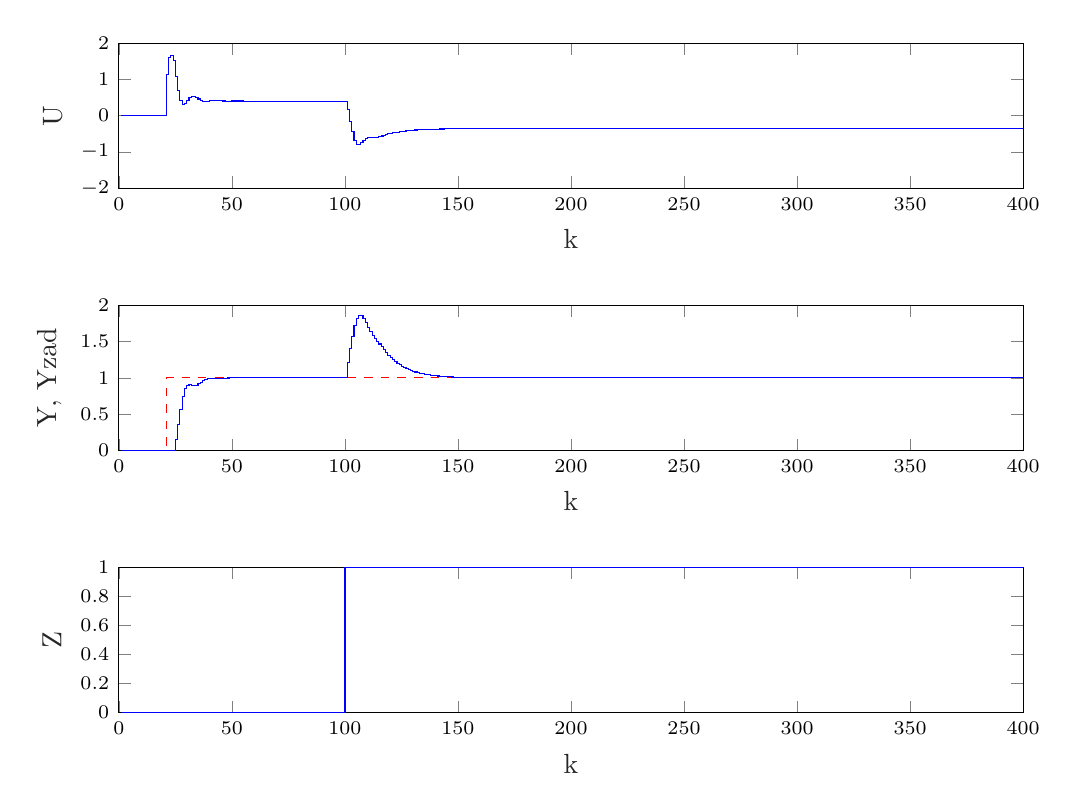
\begin{tikzpicture}

\begin{axis}[%
width=4.521in,
height=0.725in,
at={(0.758in,3.322in)},
scale only axis,
xmin=0,
xmax=400,
xlabel style={font=\color{white!15!black}},
xlabel={k},
ymin=-2,
ymax=2,
ylabel style={font=\color{white!15!black}},
ylabel={U},
axis background/.style={fill=white}
]
\addplot[const plot, color=blue, forget plot] table[row sep=crcr] {%
1	0\\
2	0\\
3	0\\
4	0\\
5	0\\
6	0\\
7	0\\
8	0\\
9	0\\
10	0\\
11	0\\
12	0\\
13	0\\
14	0\\
15	0\\
16	0\\
17	0\\
18	0\\
19	0\\
20	0\\
21	1.13124041331753\\
22	1.60739620208848\\
23	1.67029772812697\\
24	1.5088290696095\\
25	1.08258009935487\\
26	0.684037120257817\\
27	0.424015380122655\\
28	0.310055013493176\\
29	0.329911659559614\\
30	0.412055543717462\\
31	0.49284813281035\\
32	0.53826796688865\\
33	0.537912993315766\\
34	0.504308140292631\\
35	0.45877281065022\\
36	0.419410565589577\\
37	0.396275443971251\\
38	0.390196587205243\\
39	0.395737940223536\\
40	0.405530115035693\\
41	0.413556147410279\\
42	0.416831988264799\\
43	0.415363749413303\\
44	0.41100616794113\\
45	0.406084453780792\\
46	0.402349250225408\\
47	0.40052789855623\\
48	0.400422166673599\\
49	0.401311205757422\\
50	0.402400609633999\\
51	0.403135629315426\\
52	0.403312371317209\\
53	0.403020350347085\\
54	0.402499132197402\\
55	0.401993011482922\\
56	0.401657765772953\\
57	0.40153450897489\\
58	0.401575545994931\\
59	0.40169360029823\\
60	0.40180770201165\\
61	0.401870068243431\\
62	0.401871046600647\\
63	0.40182832958733\\
64	0.401770153994924\\
65	0.401720848379131\\
66	0.401693163682481\\
67	0.401687705971358\\
68	0.401697066358232\\
69	0.40171140175517\\
70	0.401722879568028\\
71	0.401727766843836\\
72	0.401726257840868\\
73	0.401720930851284\\
74	0.401714902237765\\
75	0.401710465406525\\
76	0.401708535593691\\
77	0.401708807856827\\
78	0.40171030785626\\
79	0.401711988442695\\
80	0.401713135670161\\
81	0.401713504677854\\
82	0.401713234372025\\
83	0.401712653194794\\
84	0.401712087119452\\
85	0.401711739451988\\
86	0.401711660141687\\
87	0.401711782952107\\
88	0.401711991877851\\
89	0.401712181631659\\
90	0.401712292121399\\
91	0.40171231376668\\
92	0.401712272378503\\
93	0.401712206636815\\
94	0.401712149141236\\
95	0.401712116674031\\
96	0.401712109863984\\
97	0.401712118919425\\
98	0.401712131093258\\
99	0.401712136499113\\
100	0.401712130744792\\
101	0.160475096441706\\
102	-0.155227652291736\\
103	-0.448906935162451\\
104	-0.675180934884802\\
105	-0.78514450680548\\
106	-0.79775571849983\\
107	-0.753479043993001\\
108	-0.689847674993846\\
109	-0.637572458106992\\
110	-0.60866408148127\\
111	-0.600213951069078\\
112	-0.602384210919803\\
113	-0.604222364160676\\
114	-0.59867579347581\\
115	-0.58402974603963\\
116	-0.562622631557903\\
117	-0.538674597540242\\
118	-0.51610906900605\\
119	-0.497249899541557\\
120	-0.482588525395148\\
121	-0.471277979545612\\
122	-0.461929868899412\\
123	-0.453312817222692\\
124	-0.444729098373045\\
125	-0.436055102826766\\
126	-0.427554394567246\\
127	-0.419616042667845\\
128	-0.412543152405001\\
129	-0.406451057971032\\
130	-0.401272705400855\\
131	-0.396830228730424\\
132	-0.392922210073268\\
133	-0.389388897915761\\
134	-0.386139535133235\\
135	-0.383145628724309\\
136	-0.380415088453847\\
137	-0.377963690683369\\
138	-0.375795257508175\\
139	-0.373894558006137\\
140	-0.372230792074506\\
141	-0.370766415881674\\
142	-0.369466031313605\\
143	-0.368301977789564\\
144	-0.367255713647973\\
145	-0.366315960261145\\
146	-0.365475418692711\\
147	-0.364727733684291\\
148	-0.364065678970316\\
149	-0.36348073631126\\
150	-0.36296366960275\\
151	-0.362505480070081\\
152	-0.362098217483783\\
153	-0.361735371222798\\
154	-0.361411823754341\\
155	-0.3611235190477\\
156	-0.360867049758833\\
157	-0.360639324402922\\
158	-0.360437389310999\\
159	-0.360258397775652\\
160	-0.360099669231182\\
161	-0.359958770759214\\
162	-0.359833571242472\\
163	-0.359722248009516\\
164	-0.359623251776699\\
165	-0.359535249880909\\
166	-0.359457069328759\\
167	-0.359387654155824\\
168	-0.35932604172824\\
169	-0.359271354597499\\
170	-0.359222800617021\\
171	-0.359179674175229\\
172	-0.359141354061853\\
173	-0.359107296767002\\
174	-0.359077026487803\\
175	-0.359050124176978\\
176	-0.359026217745981\\
177	-0.359004974587762\\
178	-0.358986096528489\\
179	-0.358969316584276\\
180	-0.358954396641799\\
181	-0.358941125322923\\
182	-0.358929315637136\\
183	-0.358918802373127\\
184	-0.358909439404964\\
185	-0.358901097153389\\
186	-0.358893660384703\\
187	-0.358887026416182\\
188	-0.358881103691134\\
189	-0.358875810625549\\
190	-0.358871074618793\\
191	-0.358866831148168\\
192	-0.35886302290861\\
193	-0.358859598994399\\
194	-0.358856514139238\\
195	-0.358853728033592\\
196	-0.358851204729446\\
197	-0.358848912130455\\
198	-0.35884682155578\\
199	-0.358844907361762\\
200	-0.358843146606656\\
201	-0.358841518747936\\
202	-0.358840005366544\\
203	-0.35883858991619\\
204	-0.358837257497522\\
205	-0.358835994657009\\
206	-0.358834789209388\\
207	-0.358833630081451\\
208	-0.358832507174231\\
209	-0.358831411240577\\
210	-0.358830333775503\\
211	-0.358829266917378\\
212	-0.358828203358605\\
213	-0.358827136264891\\
214	-0.358826059202421\\
215	-0.358824966072251\\
216	-0.358823851051213\\
217	-0.358822728285484\\
218	-0.358821693478298\\
219	-0.358821015098431\\
220	-0.358820875339334\\
221	-0.358821293019439\\
222	-0.358822128766484\\
223	-0.358825934128604\\
224	-0.3588318356639\\
225	-0.358837974762601\\
226	-0.358842794246422\\
227	-0.358844646568678\\
228	-0.358843353236184\\
229	-0.358839951032459\\
230	-0.358835913252054\\
231	-0.358832687694338\\
232	-0.358831077701203\\
233	-0.35883108240932\\
234	-0.358832133496212\\
235	-0.358833436411298\\
236	-0.358834333968723\\
237	-0.358834519274962\\
238	-0.3588340469545\\
239	-0.35883321021982\\
240	-0.358832361383505\\
241	-0.358831761478428\\
242	-0.358831509996203\\
243	-0.358831555761273\\
244	-0.358831760983533\\
245	-0.358831978360463\\
246	-0.358832107880802\\
247	-0.358832118454955\\
248	-0.35883203722303\\
249	-0.358831920648622\\
250	-0.358831823992828\\
251	-0.358831781056996\\
252	-0.358831798447756\\
253	-0.358831861827572\\
254	-0.35883194794111\\
255	-0.35883203606591\\
256	-0.358832114817531\\
257	-0.358832183298672\\
258	-0.35883224802088\\
259	-0.358832318131025\\
260	-0.358832401269863\\
261	-0.358832501385443\\
262	-0.358832618659351\\
263	-0.358832750867393\\
264	-0.358832895190927\\
265	-0.358833049657404\\
266	-0.358833213801846\\
267	-0.358833388566992\\
268	-0.35883357573602\\
269	-0.358833777265692\\
270	-0.358833994800368\\
271	-0.358834229485519\\
272	-0.358834482048472\\
273	-0.358834753026398\\
274	-0.358835043008092\\
275	-0.358835352796637\\
276	-0.358835683461094\\
277	-0.358836036297332\\
278	-0.358836412744908\\
279	-0.358836814307077\\
280	-0.358837242503841\\
281	-0.358837698865518\\
282	-0.358838184956908\\
283	-0.358838702414358\\
284	-0.358839252979488\\
285	-0.358839838520277\\
286	-0.35884046103822\\
287	-0.358841122665951\\
288	-0.35884182566185\\
289	-0.358842572407132\\
290	-0.358843365408233\\
291	-0.358844207304499\\
292	-0.358845100879409\\
293	-0.358846049072988\\
294	-0.358847054993645\\
295	-0.358848121928632\\
296	-0.358849253353312\\
297	-0.358850448728916\\
298	-0.358851686629394\\
299	-0.358852890304445\\
300	-0.358853952342117\\
301	-0.358854773000612\\
302	-0.358855293127964\\
303	-0.358854915809109\\
304	-0.35885329713519\\
305	-0.358850527938882\\
306	-0.358847020756174\\
307	-0.358843493013091\\
308	-0.358840619543226\\
309	-0.358838778213475\\
310	-0.358837990170322\\
311	-0.358837965320753\\
312	-0.358838274709084\\
313	-0.358838537619141\\
314	-0.35883853719284\\
315	-0.358838250302434\\
316	-0.358837796528938\\
317	-0.358837347454683\\
318	-0.358837043738426\\
319	-0.358836947710511\\
320	-0.358837039564531\\
321	-0.358837246046302\\
322	-0.358837480907776\\
323	-0.358837678502607\\
324	-0.358837809951923\\
325	-0.358837881052953\\
326	-0.358837918307937\\
327	-0.358837951907429\\
328	-0.358838002902951\\
329	-0.358838077983424\\
330	-0.358838171347743\\
331	-0.358838270687385\\
332	-0.358838363720884\\
333	-0.358838442662189\\
334	-0.358838505622989\\
335	-0.358838555415793\\
336	-0.358838597040159\\
337	-0.358838635206054\\
338	-0.358838672791766\\
339	-0.358838710493075\\
340	-0.358838747395235\\
341	-0.358838781947366\\
342	-0.358838812843545\\
343	-0.35883883951515\\
344	-0.358838862182026\\
345	-0.358838881591033\\
346	-0.358838898643263\\
347	-0.358838914084773\\
348	-0.358838928353443\\
349	-0.358838941585698\\
350	-0.358838953726617\\
351	-0.358838964667985\\
352	-0.358838974354196\\
353	-0.358838982828251\\
354	-0.358838990221657\\
355	-0.358838996711435\\
356	-0.358839002471644\\
357	-0.358839007639426\\
358	-0.358839012303392\\
359	-0.358839016511201\\
360	-0.358839020287173\\
361	-0.358839023650246\\
362	-0.358839026625733\\
363	-0.358839029248902\\
364	-0.358839031562056\\
365	-0.3588390336086\\
366	-0.358839035427465\\
367	-0.358839037049961\\
368	-0.358839038499478\\
369	-0.35883903979328\\
370	-0.358839040945092\\
371	-0.35883904196735\\
372	-0.358839042872473\\
373	-0.358839043673107\\
374	-0.358839044381676\\
375	-0.358839045009694\\
376	-0.358839045567239\\
377	-0.358839046062758\\
378	-0.358839046503215\\
379	-0.358839046894428\\
380	-0.35883904724145\\
381	-0.358839047548863\\
382	-0.358839047820932\\
383	-0.358839048061637\\
384	-0.358839048274632\\
385	-0.358839048463196\\
386	-0.358839048630203\\
387	-0.358839048778141\\
388	-0.358839048909163\\
389	-0.358839049025149\\
390	-0.358839049127767\\
391	-0.358839049218526\\
392	-0.358839049298792\\
393	-0.358839049369808\\
394	-0.358839049432694\\
395	-0.358839049488454\\
396	-0.358839049537981\\
397	-0.358839049582066\\
398	-0.358839049621419\\
399	-0.358839049656677\\
400	-0.358839049688416\\
};
\end{axis}

\begin{axis}[%
width=4.521in,
height=0.725in,
at={(0.758in,2.011in)},
scale only axis,
xmin=0,
xmax=400,
xlabel style={font=\color{white!15!black}},
xlabel={k},
ymin=0,
ymax=2,
ylabel style={font=\color{white!15!black}},
ylabel={Y, Yzad},
axis background/.style={fill=white}
]
\addplot[const plot, color=red, dashed, forget plot] table[row sep=crcr] {%
1	0\\
2	0\\
3	0\\
4	0\\
5	0\\
6	0\\
7	0\\
8	0\\
9	0\\
10	0\\
11	0\\
12	0\\
13	0\\
14	0\\
15	0\\
16	0\\
17	0\\
18	0\\
19	0\\
20	0\\
21	1\\
22	1\\
23	1\\
24	1\\
25	1\\
26	1\\
27	1\\
28	1\\
29	1\\
30	1\\
31	1\\
32	1\\
33	1\\
34	1\\
35	1\\
36	1\\
37	1\\
38	1\\
39	1\\
40	1\\
41	1\\
42	1\\
43	1\\
44	1\\
45	1\\
46	1\\
47	1\\
48	1\\
49	1\\
50	1\\
51	1\\
52	1\\
53	1\\
54	1\\
55	1\\
56	1\\
57	1\\
58	1\\
59	1\\
60	1\\
61	1\\
62	1\\
63	1\\
64	1\\
65	1\\
66	1\\
67	1\\
68	1\\
69	1\\
70	1\\
71	1\\
72	1\\
73	1\\
74	1\\
75	1\\
76	1\\
77	1\\
78	1\\
79	1\\
80	1\\
81	1\\
82	1\\
83	1\\
84	1\\
85	1\\
86	1\\
87	1\\
88	1\\
89	1\\
90	1\\
91	1\\
92	1\\
93	1\\
94	1\\
95	1\\
96	1\\
97	1\\
98	1\\
99	1\\
100	1\\
101	1\\
102	1\\
103	1\\
104	1\\
105	1\\
106	1\\
107	1\\
108	1\\
109	1\\
110	1\\
111	1\\
112	1\\
113	1\\
114	1\\
115	1\\
116	1\\
117	1\\
118	1\\
119	1\\
120	1\\
121	1\\
122	1\\
123	1\\
124	1\\
125	1\\
126	1\\
127	1\\
128	1\\
129	1\\
130	1\\
131	1\\
132	1\\
133	1\\
134	1\\
135	1\\
136	1\\
137	1\\
138	1\\
139	1\\
140	1\\
141	1\\
142	1\\
143	1\\
144	1\\
145	1\\
146	1\\
147	1\\
148	1\\
149	1\\
150	1\\
151	1\\
152	1\\
153	1\\
154	1\\
155	1\\
156	1\\
157	1\\
158	1\\
159	1\\
160	1\\
161	1\\
162	1\\
163	1\\
164	1\\
165	1\\
166	1\\
167	1\\
168	1\\
169	1\\
170	1\\
171	1\\
172	1\\
173	1\\
174	1\\
175	1\\
176	1\\
177	1\\
178	1\\
179	1\\
180	1\\
181	1\\
182	1\\
183	1\\
184	1\\
185	1\\
186	1\\
187	1\\
188	1\\
189	1\\
190	1\\
191	1\\
192	1\\
193	1\\
194	1\\
195	1\\
196	1\\
197	1\\
198	1\\
199	1\\
200	1\\
201	1\\
202	1\\
203	1\\
204	1\\
205	1\\
206	1\\
207	1\\
208	1\\
209	1\\
210	1\\
211	1\\
212	1\\
213	1\\
214	1\\
215	1\\
216	1\\
217	1\\
218	1\\
219	1\\
220	1\\
221	1\\
222	1\\
223	1\\
224	1\\
225	1\\
226	1\\
227	1\\
228	1\\
229	1\\
230	1\\
231	1\\
232	1\\
233	1\\
234	1\\
235	1\\
236	1\\
237	1\\
238	1\\
239	1\\
240	1\\
241	1\\
242	1\\
243	1\\
244	1\\
245	1\\
246	1\\
247	1\\
248	1\\
249	1\\
250	1\\
251	1\\
252	1\\
253	1\\
254	1\\
255	1\\
256	1\\
257	1\\
258	1\\
259	1\\
260	1\\
261	1\\
262	1\\
263	1\\
264	1\\
265	1\\
266	1\\
267	1\\
268	1\\
269	1\\
270	1\\
271	1\\
272	1\\
273	1\\
274	1\\
275	1\\
276	1\\
277	1\\
278	1\\
279	1\\
280	1\\
281	1\\
282	1\\
283	1\\
284	1\\
285	1\\
286	1\\
287	1\\
288	1\\
289	1\\
290	1\\
291	1\\
292	1\\
293	1\\
294	1\\
295	1\\
296	1\\
297	1\\
298	1\\
299	1\\
300	1\\
301	1\\
302	1\\
303	1\\
304	1\\
305	1\\
306	1\\
307	1\\
308	1\\
309	1\\
310	1\\
311	1\\
312	1\\
313	1\\
314	1\\
315	1\\
316	1\\
317	1\\
318	1\\
319	1\\
320	1\\
321	1\\
322	1\\
323	1\\
324	1\\
325	1\\
326	1\\
327	1\\
328	1\\
329	1\\
330	1\\
331	1\\
332	1\\
333	1\\
334	1\\
335	1\\
336	1\\
337	1\\
338	1\\
339	1\\
340	1\\
341	1\\
342	1\\
343	1\\
344	1\\
345	1\\
346	1\\
347	1\\
348	1\\
349	1\\
350	1\\
351	1\\
352	1\\
353	1\\
354	1\\
355	1\\
356	1\\
357	1\\
358	1\\
359	1\\
360	1\\
361	1\\
362	1\\
363	1\\
364	1\\
365	1\\
366	1\\
367	1\\
368	1\\
369	1\\
370	1\\
371	1\\
372	1\\
373	1\\
374	1\\
375	1\\
376	1\\
377	1\\
378	1\\
379	1\\
380	1\\
381	1\\
382	1\\
383	1\\
384	1\\
385	1\\
386	1\\
387	1\\
388	1\\
389	1\\
390	1\\
391	1\\
392	1\\
393	1\\
394	1\\
395	1\\
396	1\\
397	1\\
398	1\\
399	1\\
400	1\\
};
\addplot[const plot, color=blue, forget plot] table[row sep=crcr] {%
1	0\\
2	0\\
3	0\\
4	0\\
5	0\\
6	0\\
7	0\\
8	0\\
9	0\\
10	0\\
11	0\\
12	0\\
13	0\\
14	0\\
15	0\\
16	0\\
17	0\\
18	0\\
19	0\\
20	0\\
21	0\\
22	0\\
23	0\\
24	0\\
25	0.152830579839198\\
26	0.361723685979986\\
27	0.567813252929803\\
28	0.740934525440941\\
29	0.847095360437015\\
30	0.893658115143514\\
31	0.90255973864811\\
32	0.895570671873684\\
33	0.89163036498361\\
34	0.898990405246294\\
35	0.91685828271975\\
36	0.939887677878803\\
37	0.961615803129477\\
38	0.977621370527924\\
39	0.986602460199098\\
40	0.989773437013205\\
41	0.989641380644215\\
42	0.988689847199495\\
43	0.988533654813312\\
44	0.989704626042417\\
45	0.991892848316057\\
46	0.994401945347177\\
47	0.996573965969035\\
48	0.998037076898529\\
49	0.998753666950623\\
50	0.998924656597726\\
51	0.998838350857697\\
52	0.998740665168325\\
53	0.998766808279368\\
54	0.998937329483177\\
55	0.999196697549384\\
56	0.999464818354491\\
57	0.999678006297738\\
58	0.999808372281484\\
59	0.999862529279366\\
60	0.999867769339971\\
61	0.999855454910885\\
62	0.999848800913543\\
63	0.999857968169211\\
64	0.999881621834702\\
65	0.999912037309881\\
66	0.999940598025195\\
67	0.999961538784302\\
68	0.999973216807206\\
69	0.999977361349574\\
70	0.999977327623101\\
71	0.999976368399375\\
72	0.999976556980123\\
73	0.999978522354457\\
74	0.999981799158156\\
75	0.999985440953475\\
76	0.999988577040411\\
77	0.999990730653257\\
78	0.99999187053213\\
79	0.999992275801492\\
80	0.999992333120867\\
81	0.99999236613075\\
82	0.999992548519416\\
83	0.999992902381439\\
84	0.999993351510946\\
85	0.999993790164412\\
86	0.999994136571704\\
87	0.999994357305398\\
88	0.999994464385011\\
89	0.999994496292151\\
90	0.999994495860299\\
91	0.999994494377281\\
92	0.999994505516522\\
93	0.999994527765157\\
94	0.999994551375948\\
95	0.999994565659013\\
96	0.999994563834085\\
97	0.999994544575335\\
98	0.999994510910527\\
99	0.999994467862375\\
100	0.999994420170427\\
101	1.2132443709093\\
102	1.40256084618896\\
103	1.57062529004848\\
104	1.71981897655279\\
105	1.81966547754278\\
106	1.8637451689591\\
107	1.85891332261007\\
108	1.81768975773037\\
109	1.75843906801614\\
110	1.69589547195372\\
111	1.63846178402568\\
112	1.58895517062073\\
113	1.54583756580882\\
114	1.50598360490527\\
115	1.46678747206765\\
116	1.42707577036301\\
117	1.38718490980657\\
118	1.348356338578\\
119	1.31196975862356\\
120	1.27899098703012\\
121	1.24974270962403\\
122	1.22398166164581\\
123	1.20114740315328\\
124	1.18062887669876\\
125	1.16194960620771\\
126	1.14483502411862\\
127	1.12918163079815\\
128	1.11497678959748\\
129	1.10221726102389\\
130	1.09085728373044\\
131	1.08079471426123\\
132	1.0718863975045\\
133	1.06397638178213\\
134	1.05692181090698\\
135	1.05060768338761\\
136	1.04494896849931\\
137	1.03988374687288\\
138	1.03536298560428\\
139	1.03134173631942\\
140	1.02777426846738\\
141	1.02461329044278\\
142	1.02181186353991\\
143	1.0193261473911\\
144	1.01711750486686\\
145	1.0151532817726\\
146	1.01340632646465\\
147	1.0118537649348\\
148	1.01047564216144\\
149	1.00925387584049\\
150	1.00817169980629\\
151	1.00721353843996\\
152	1.00636512480624\\
153	1.00561366197075\\
154	1.00494789154458\\
155	1.00435802371356\\
156	1.00383555634089\\
157	1.00337304648067\\
158	1.00296389650735\\
159	1.00260219303927\\
160	1.00228260718037\\
161	1.00200034231544\\
162	1.00175110629278\\
163	1.00153108707046\\
164	1.00133691972357\\
165	1.00116564248423\\
166	1.00101464629868\\
167	1.00088162484479\\
168	1.00076453077395\\
169	1.00066154091097\\
170	1.0005710300742\\
171	1.00049155122427\\
172	1.0004218191359\\
173	1.00036069538563\\
174	1.00030717354356\\
175	1.00026036447386\\
176	1.00021948225239\\
177	1.00018383133766\\
178	1.00015279541886\\
179	1.00012582802116\\
180	1.00010244465389\\
181	1.0000822161376\\
182	1.00006476274668\\
183	1.00004974890549\\
184	1.00003687830577\\
185	1.00002588941804\\
186	1.00001655142211\\
187	1.00000866058526\\
188	1.00000203708943\\
189	0.99999652227481\\
190	0.999991976242589\\
191	0.999988275752588\\
192	0.999985312358441\\
193	0.99998299073861\\
194	0.999981227197324\\
195	0.999979948321016\\
196	0.999979089781165\\
197	0.999978595274731\\
198	0.999978415591127\\
199	0.999978507792205\\
200	0.999978834490695\\
201	0.999979363213196\\
202	0.999980065835839\\
203	0.999980918083193\\
204	0.999981899083283\\
205	0.999982990973088\\
206	0.999984178549808\\
207	0.999985448963479\\
208	0.999986791446622\\
209	0.999988197076721\\
210	0.999989658567598\\
211	0.999991170086115\\
212	0.999992727091156\\
213	0.999994326192311\\
214	0.999995965026082\\
215	0.999997642147782\\
216	0.999999356937458\\
217	1.00000110951837\\
218	1.0000029006867\\
219	1.00000473185114\\
220	1.00000660498144\\
221	1.00000851989692\\
222	1.00001046337925\\
223	1.00001238655029\\
224	1.00001421846857\\
225	1.00001588940602\\
226	1.0000173521645\\
227	1.00001821732324\\
228	1.00001823447259\\
229	1.0000174178056\\
230	1.00001599109273\\
231	1.00001438855827\\
232	1.00001304502677\\
233	1.0000122317009\\
234	1.00001200603339\\
235	1.00001222673127\\
236	1.00001265157498\\
237	1.00001305153237\\
238	1.0000132867176\\
239	1.00001333214005\\
240	1.00001325293664\\
241	1.00001315217418\\
242	1.00001311995643\\
243	1.00001320189077\\
244	1.00001339350974\\
245	1.00001365531157\\
246	1.00001393648052\\
247	1.00001419585582\\
248	1.00001441311297\\
249	1.00001458892337\\
250	1.00001473743049\\
251	1.0000148762103\\
252	1.00001501821872\\
253	1.00001516807993\\
254	1.00001532269943\\
255	1.000015474581\\
256	1.00001561573911\\
257	1.00001574055535\\
258	1.00001584685555\\
259	1.0000159353816\\
260	1.00001600837231\\
261	1.00001606806576\\
262	1.00001611569842\\
263	1.00001615120338\\
264	1.00001617348433\\
265	1.00001618097026\\
266	1.00001617215006\\
267	1.00001614589437\\
268	1.00001610151534\\
269	1.00001603862853\\
270	1.00001595693286\\
271	1.00001585601591\\
272	1.00001573524653\\
273	1.00001559376314\\
274	1.0000154305285\\
275	1.00001524440663\\
276	1.00001503422465\\
277	1.00001479880052\\
278	1.00001453693659\\
279	1.00001424739151\\
280	1.00001392884666\\
281	1.00001357987976\\
282	1.00001319895105\\
283	1.00001278440105\\
284	1.00001233445482\\
285	1.00001184722683\\
286	1.00001132072228\\
287	1.00001075283337\\
288	1.00001014133124\\
289	1.00000948385543\\
290	1.000008777903\\
291	1.00000802081853\\
292	1.00000720978542\\
293	1.00000634181801\\
294	1.00000541375384\\
295	1.0000044222453\\
296	1.00000336375016\\
297	1.00000223452101\\
298	1.0000010305936\\
299	0.999999747774459\\
300	0.999998381627918\\
301	0.999996928031519\\
302	0.999995385981003\\
303	0.999993764895975\\
304	0.999992088198458\\
305	0.999990391519052\\
306	0.999988716552408\\
307	0.999987183380324\\
308	0.999985952050134\\
309	0.99998516167722\\
310	0.999984888112166\\
311	0.999985106169794\\
312	0.999985700847536\\
313	0.999986512305169\\
314	0.999987386486151\\
315	0.999988216857091\\
316	0.999988960601018\\
317	0.999989628655931\\
318	0.999990260670539\\
319	0.999990897277653\\
320	0.999991560759736\\
321	0.99999224901488\\
322	0.999992941052821\\
323	0.999993608598648\\
324	0.999994227583823\\
325	0.999994785139912\\
326	0.999995280748592\\
327	0.999995722790422\\
328	0.999996123096035\\
329	0.99999649207441\\
330	0.999996835992116\\
331	0.999997156698734\\
332	0.999997453100239\\
333	0.999997723258497\\
334	0.999997966124308\\
335	0.999998182368473\\
336	0.999998374285091\\
337	0.999998545096372\\
338	0.999998698105578\\
339	0.999998836057464\\
340	0.999998960872933\\
341	0.999999073732658\\
342	0.999999175364542\\
343	0.999999266363041\\
344	0.999999347413963\\
345	0.999999419375462\\
346	0.999999483235616\\
347	0.999999540005788\\
348	0.999999590612831\\
349	0.999999635832451\\
350	0.99999967627654\\
351	0.999999712422977\\
352	0.999999744664516\\
353	0.999999773354115\\
354	0.999999798832949\\
355	0.999999821438253\\
356	0.999999841496428\\
357	0.999999859310315\\
358	0.999999875148514\\
359	0.999999889241092\\
360	0.99999990178207\\
361	0.999999912936367\\
362	0.999999922847937\\
363	0.999999931646436\\
364	0.999999939451157\\
365	0.999999946372321\\
366	0.999999952510712\\
367	0.999999957956845\\
368	0.999999962790576\\
369	0.999999967081531\\
370	0.999999970890271\\
371	0.999999974269811\\
372	0.999999977267105\\
373	0.999999979924201\\
374	0.999999982278989\\
375	0.999999984365604\\
376	0.999999986214628\\
377	0.999999987853261\\
378	0.99999998930553\\
379	0.999999990592589\\
380	0.999999991733068\\
381	0.999999992743433\\
382	0.999999993638302\\
383	0.999999994430706\\
384	0.999999995132273\\
385	0.999999995753375\\
386	0.999999996303234\\
387	0.99999999679003\\
388	0.999999997220995\\
389	0.99999999760252\\
390	0.999999997940258\\
391	0.99999999823921\\
392	0.999999998503813\\
393	0.999999998738003\\
394	0.999999998945274\\
395	0.999999999128723\\
396	0.99999999929109\\
397	0.999999999434798\\
398	0.999999999561983\\
399	0.999999999674526\\
400	0.999999999774085\\
};
\end{axis}

\begin{axis}[%
width=4.521in,
height=0.725in,
at={(0.758in,0.7in)},
scale only axis,
xmin=0,
xmax=400,
xlabel style={font=\color{white!15!black}},
xlabel={k},
ymin=0,
ymax=1,
ylabel style={font=\color{white!15!black}},
ylabel={Z},
axis background/.style={fill=white}
]
\addplot[const plot, color=blue, forget plot] table[row sep=crcr] {%
1	0\\
2	0\\
3	0\\
4	0\\
5	0\\
6	0\\
7	0\\
8	0\\
9	0\\
10	0\\
11	0\\
12	0\\
13	0\\
14	0\\
15	0\\
16	0\\
17	0\\
18	0\\
19	0\\
20	0\\
21	0\\
22	0\\
23	0\\
24	0\\
25	0\\
26	0\\
27	0\\
28	0\\
29	0\\
30	0\\
31	0\\
32	0\\
33	0\\
34	0\\
35	0\\
36	0\\
37	0\\
38	0\\
39	0\\
40	0\\
41	0\\
42	0\\
43	0\\
44	0\\
45	0\\
46	0\\
47	0\\
48	0\\
49	0\\
50	0\\
51	0\\
52	0\\
53	0\\
54	0\\
55	0\\
56	0\\
57	0\\
58	0\\
59	0\\
60	0\\
61	0\\
62	0\\
63	0\\
64	0\\
65	0\\
66	0\\
67	0\\
68	0\\
69	0\\
70	0\\
71	0\\
72	0\\
73	0\\
74	0\\
75	0\\
76	0\\
77	0\\
78	0\\
79	0\\
80	0\\
81	0\\
82	0\\
83	0\\
84	0\\
85	0\\
86	0\\
87	0\\
88	0\\
89	0\\
90	0\\
91	0\\
92	0\\
93	0\\
94	0\\
95	0\\
96	0\\
97	0\\
98	0\\
99	0\\
100	1\\
101	1\\
102	1\\
103	1\\
104	1\\
105	1\\
106	1\\
107	1\\
108	1\\
109	1\\
110	1\\
111	1\\
112	1\\
113	1\\
114	1\\
115	1\\
116	1\\
117	1\\
118	1\\
119	1\\
120	1\\
121	1\\
122	1\\
123	1\\
124	1\\
125	1\\
126	1\\
127	1\\
128	1\\
129	1\\
130	1\\
131	1\\
132	1\\
133	1\\
134	1\\
135	1\\
136	1\\
137	1\\
138	1\\
139	1\\
140	1\\
141	1\\
142	1\\
143	1\\
144	1\\
145	1\\
146	1\\
147	1\\
148	1\\
149	1\\
150	1\\
151	1\\
152	1\\
153	1\\
154	1\\
155	1\\
156	1\\
157	1\\
158	1\\
159	1\\
160	1\\
161	1\\
162	1\\
163	1\\
164	1\\
165	1\\
166	1\\
167	1\\
168	1\\
169	1\\
170	1\\
171	1\\
172	1\\
173	1\\
174	1\\
175	1\\
176	1\\
177	1\\
178	1\\
179	1\\
180	1\\
181	1\\
182	1\\
183	1\\
184	1\\
185	1\\
186	1\\
187	1\\
188	1\\
189	1\\
190	1\\
191	1\\
192	1\\
193	1\\
194	1\\
195	1\\
196	1\\
197	1\\
198	1\\
199	1\\
200	1\\
201	1\\
202	1\\
203	1\\
204	1\\
205	1\\
206	1\\
207	1\\
208	1\\
209	1\\
210	1\\
211	1\\
212	1\\
213	1\\
214	1\\
215	1\\
216	1\\
217	1\\
218	1\\
219	1\\
220	1\\
221	1\\
222	1\\
223	1\\
224	1\\
225	1\\
226	1\\
227	1\\
228	1\\
229	1\\
230	1\\
231	1\\
232	1\\
233	1\\
234	1\\
235	1\\
236	1\\
237	1\\
238	1\\
239	1\\
240	1\\
241	1\\
242	1\\
243	1\\
244	1\\
245	1\\
246	1\\
247	1\\
248	1\\
249	1\\
250	1\\
251	1\\
252	1\\
253	1\\
254	1\\
255	1\\
256	1\\
257	1\\
258	1\\
259	1\\
260	1\\
261	1\\
262	1\\
263	1\\
264	1\\
265	1\\
266	1\\
267	1\\
268	1\\
269	1\\
270	1\\
271	1\\
272	1\\
273	1\\
274	1\\
275	1\\
276	1\\
277	1\\
278	1\\
279	1\\
280	1\\
281	1\\
282	1\\
283	1\\
284	1\\
285	1\\
286	1\\
287	1\\
288	1\\
289	1\\
290	1\\
291	1\\
292	1\\
293	1\\
294	1\\
295	1\\
296	1\\
297	1\\
298	1\\
299	1\\
300	1\\
301	1\\
302	1\\
303	1\\
304	1\\
305	1\\
306	1\\
307	1\\
308	1\\
309	1\\
310	1\\
311	1\\
312	1\\
313	1\\
314	1\\
315	1\\
316	1\\
317	1\\
318	1\\
319	1\\
320	1\\
321	1\\
322	1\\
323	1\\
324	1\\
325	1\\
326	1\\
327	1\\
328	1\\
329	1\\
330	1\\
331	1\\
332	1\\
333	1\\
334	1\\
335	1\\
336	1\\
337	1\\
338	1\\
339	1\\
340	1\\
341	1\\
342	1\\
343	1\\
344	1\\
345	1\\
346	1\\
347	1\\
348	1\\
349	1\\
350	1\\
351	1\\
352	1\\
353	1\\
354	1\\
355	1\\
356	1\\
357	1\\
358	1\\
359	1\\
360	1\\
361	1\\
362	1\\
363	1\\
364	1\\
365	1\\
366	1\\
367	1\\
368	1\\
369	1\\
370	1\\
371	1\\
372	1\\
373	1\\
374	1\\
375	1\\
376	1\\
377	1\\
378	1\\
379	1\\
380	1\\
381	1\\
382	1\\
383	1\\
384	1\\
385	1\\
386	1\\
387	1\\
388	1\\
389	1\\
390	1\\
391	1\\
392	1\\
393	1\\
394	1\\
395	1\\
396	1\\
397	1\\
398	1\\
399	1\\
400	1\\
};
\end{axis}
\end{tikzpicture}%
	\label{5przebieg}
\end{figure}

\subsection{Z uwzględnieniem zakłóceń}

W trybie pracy algorytmu z uwzględnianiem zakłóceń otrzymano wskaźnik jakości $e$~=~\num{7.1838}. Przebieg przedstawiono na rysunku \ref{5zprzebieg}

\begin{figure}
	
	\centering
	\caption{ Przebieg symulacji algorytmu DMC dla skoku zakłócenia z uwzględnianiem zakłóceń }
	% This file was created by matlab2tikz.
%
%The latest updates can be retrieved from
%  http://www.mathworks.com/matlabcentral/fileexchange/22022-matlab2tikz-matlab2tikz
%where you can also make suggestions and rate matlab2tikz.
%
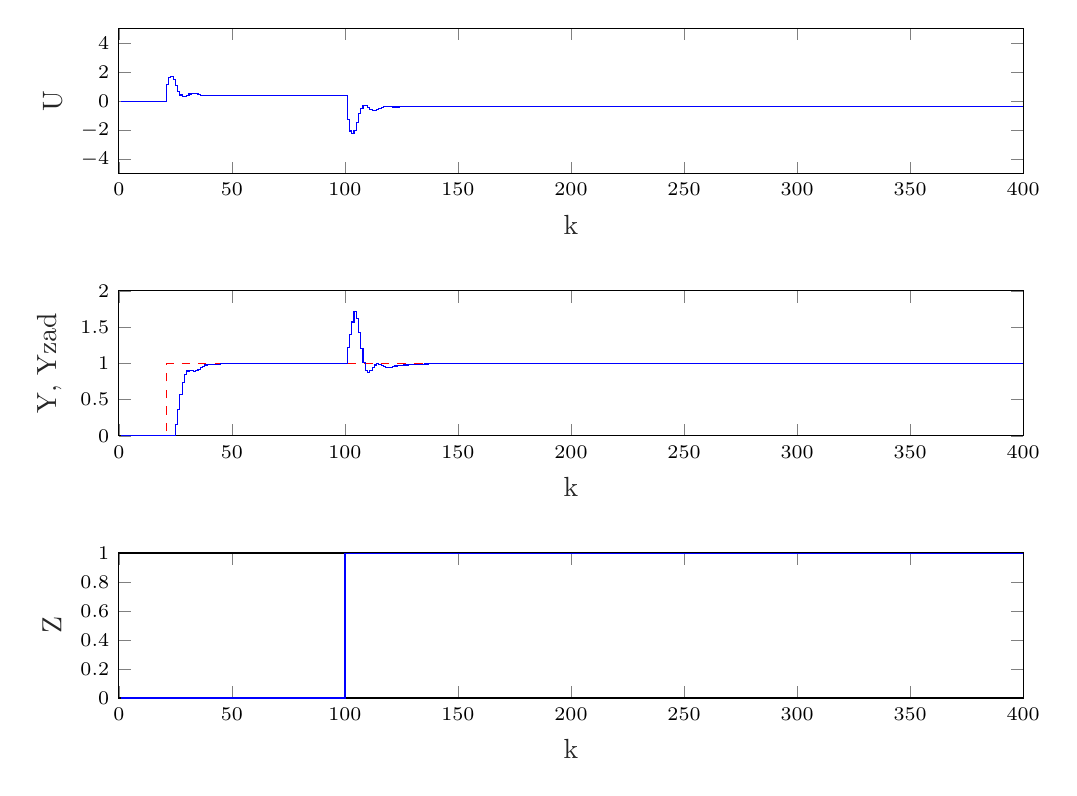
\begin{tikzpicture}

\begin{axis}[%
width=4.521in,
height=0.725in,
at={(0.758in,3.322in)},
scale only axis,
xmin=0,
xmax=400,
xlabel style={font=\color{white!15!black}},
xlabel={k},
ymin=-5,
ymax=5,
ylabel style={font=\color{white!15!black}},
ylabel={U},
axis background/.style={fill=white}
]
\addplot[const plot, color=blue, forget plot] table[row sep=crcr] {%
1	0\\
2	0\\
3	0\\
4	0\\
5	0\\
6	0\\
7	0\\
8	0\\
9	0\\
10	0\\
11	0\\
12	0\\
13	0\\
14	0\\
15	0\\
16	0\\
17	0\\
18	0\\
19	0\\
20	0\\
21	1.13124041331753\\
22	1.60739620208848\\
23	1.67029772812697\\
24	1.5088290696095\\
25	1.08258009935487\\
26	0.684037120257817\\
27	0.424015380122655\\
28	0.310055013493176\\
29	0.329911659559614\\
30	0.412055543717462\\
31	0.49284813281035\\
32	0.53826796688865\\
33	0.537912993315766\\
34	0.504308140292631\\
35	0.45877281065022\\
36	0.419410565589577\\
37	0.396275443971251\\
38	0.390196587205243\\
39	0.395737940223536\\
40	0.405530115035693\\
41	0.413556147410279\\
42	0.416831988264799\\
43	0.415363749413303\\
44	0.41100616794113\\
45	0.406084453780792\\
46	0.402349250225408\\
47	0.40052789855623\\
48	0.400422166673599\\
49	0.401311205757422\\
50	0.402400609633999\\
51	0.403135629315426\\
52	0.403312371317209\\
53	0.403020350347085\\
54	0.402499132197402\\
55	0.401993011482922\\
56	0.401657765772953\\
57	0.40153450897489\\
58	0.401575545994931\\
59	0.40169360029823\\
60	0.40180770201165\\
61	0.401870068243431\\
62	0.401871046600647\\
63	0.40182832958733\\
64	0.401770153994924\\
65	0.401720848379131\\
66	0.401693163682481\\
67	0.401687705971358\\
68	0.401697066358232\\
69	0.40171140175517\\
70	0.401722879568028\\
71	0.401727766843836\\
72	0.401726257840868\\
73	0.401720930851284\\
74	0.401714902237765\\
75	0.401710465406525\\
76	0.401708535593691\\
77	0.401708807856827\\
78	0.40171030785626\\
79	0.401711988442695\\
80	0.401713135670161\\
81	0.401713504677854\\
82	0.401713234372025\\
83	0.401712653194794\\
84	0.401712087119452\\
85	0.401711739451988\\
86	0.401711660141687\\
87	0.401711782952107\\
88	0.401711991877851\\
89	0.401712181631659\\
90	0.401712292121399\\
91	0.40171231376668\\
92	0.401712272378503\\
93	0.401712206636815\\
94	0.401712149141236\\
95	0.401712116674031\\
96	0.401712109863984\\
97	0.401712118919425\\
98	0.401712131093258\\
99	0.401712136499113\\
100	0.401712130744792\\
101	-1.2965066330836\\
102	-2.06195373752893\\
103	-2.22261849637635\\
104	-2.041788843556\\
105	-1.44928017846666\\
106	-0.873919226005589\\
107	-0.48606105540711\\
108	-0.305534856057798\\
109	-0.321846923103503\\
110	-0.434065855201892\\
111	-0.54917611835704\\
112	-0.615489711647571\\
113	-0.615322158161232\\
114	-0.565174697077588\\
115	-0.495571310547111\\
116	-0.433330003762849\\
117	-0.394035910391747\\
118	-0.379820347771811\\
119	-0.383346341509407\\
120	-0.394038203243644\\
121	-0.402965508475143\\
122	-0.405469856215254\\
123	-0.401268198875585\\
124	-0.392885862513716\\
125	-0.383666690584602\\
126	-0.376212631342341\\
127	-0.371670757137998\\
128	-0.369824982898458\\
129	-0.369656574731387\\
130	-0.369996922103697\\
131	-0.369998896396801\\
132	-0.369318835740146\\
133	-0.368048638863415\\
134	-0.366514249736603\\
135	-0.365063227897577\\
136	-0.363923342469196\\
137	-0.363157881214372\\
138	-0.36269846697638\\
139	-0.362414795806124\\
140	-0.362182035707313\\
141	-0.361921913437437\\
142	-0.36161199042742\\
143	-0.361271338107681\\
144	-0.360936489849796\\
145	-0.360640033167608\\
146	-0.360398705072651\\
147	-0.360211849849388\\
148	-0.360066980747744\\
149	-0.359947776562257\\
150	-0.359840665630096\\
151	-0.359738082637506\\
152	-0.35963841025327\\
153	-0.359543832625656\\
154	-0.359457646021309\\
155	-0.359382205546912\\
156	-0.359318021741173\\
157	-0.359263910846528\\
158	-0.359217751605217\\
159	-0.359177343373064\\
160	-0.359141009074329\\
161	-0.359107811544847\\
162	-0.359077442490809\\
163	-0.359049942196655\\
164	-0.359025412598024\\
165	-0.359003829399278\\
166	-0.358984984014495\\
167	-0.358968527354513\\
168	-0.358954060533666\\
169	-0.35894122066041\\
170	-0.358929730852197\\
171	-0.358919408212067\\
172	-0.358910141361152\\
173	-0.358901856153608\\
174	-0.35889448579854\\
175	-0.358887954122458\\
176	-0.358882172745955\\
177	-0.358877047616433\\
178	-0.358872488630207\\
179	-0.358868417291093\\
180	-0.358864769971388\\
181	-0.358861496888207\\
182	-0.358858558474696\\
183	-0.358855921196655\\
184	-0.358853554343279\\
185	-0.358851428425806\\
186	-0.358849515015792\\
187	-0.358847787406338\\
188	-0.358846221420144\\
189	-0.358844795897081\\
190	-0.358843492696187\\
191	-0.358842296297447\\
192	-0.358841193214664\\
193	-0.358840171431643\\
194	-0.358839219995547\\
195	-0.358838328801537\\
196	-0.358837488526396\\
197	-0.358836690635193\\
198	-0.35883592739107\\
199	-0.358835191827129\\
200	-0.358834477672266\\
201	-0.358833779246146\\
202	-0.358833091347337\\
203	-0.358832409155003\\
204	-0.358831728154498\\
205	-0.3588310440867\\
206	-0.358830352914149\\
207	-0.358829650795052\\
208	-0.358828934058032\\
209	-0.358828199174132\\
210	-0.358827442725943\\
211	-0.35882666137584\\
212	-0.358825851835726\\
213	-0.358825010839991\\
214	-0.358824135122237\\
215	-0.358823221395253\\
216	-0.358822266333227\\
217	-0.35882128630202\\
218	-0.358820378979023\\
219	-0.358819814589547\\
220	-0.358819776890272\\
221	-0.358820286090915\\
222	-0.358821204057572\\
223	-0.358825083440865\\
224	-0.358831051780879\\
225	-0.358837251343122\\
226	-0.358842125730213\\
227	-0.358844028092926\\
228	-0.358842780561746\\
229	-0.358839420478601\\
230	-0.358835421638723\\
231	-0.358832232291134\\
232	-0.358830656182317\\
233	-0.358830692813812\\
234	-0.35883177419307\\
235	-0.358833106068771\\
236	-0.358834031527477\\
237	-0.358834243924633\\
238	-0.358833798113299\\
239	-0.358832987516844\\
240	-0.358832164643489\\
241	-0.358831590708675\\
242	-0.358831365375492\\
243	-0.358831437630541\\
244	-0.358831669838178\\
245	-0.358831914844105\\
246	-0.358832072780391\\
247	-0.358832112697097\\
248	-0.358832061871432\\
249	-0.358831976902581\\
250	-0.358831913186682\\
251	-0.358831904660474\\
252	-0.358831958067181\\
253	-0.35883205920787\\
254	-0.35883218496858\\
255	-0.358832314771742\\
256	-0.358832437382026\\
257	-0.358832552056177\\
258	-0.358832665465396\\
259	-0.358832786922503\\
260	-0.358832924241179\\
261	-0.358833081550048\\
262	-0.358833259219618\\
263	-0.35883345522365\\
264	-0.358833666951213\\
265	-0.358833892647954\\
266	-0.358834132078323\\
267	-0.3588343864265\\
268	-0.358834657729916\\
269	-0.358834948213234\\
270	-0.358835259803231\\
271	-0.358835593943214\\
272	-0.358835951674714\\
273	-0.358836333866464\\
274	-0.358836741457212\\
275	-0.358837175619475\\
276	-0.358837637812362\\
277	-0.35883812974361\\
278	-0.358838653287701\\
279	-0.358839210407208\\
280	-0.358839803107211\\
281	-0.358840433430329\\
282	-0.358841103482413\\
283	-0.358841815471215\\
284	-0.358842571741802\\
285	-0.358843374799415\\
286	-0.358844227318485\\
287	-0.358845132142212\\
288	-0.358846092279216\\
289	-0.358847110902781\\
290	-0.358848191355488\\
291	-0.358849337159281\\
292	-0.358850552029149\\
293	-0.358851839888145\\
294	-0.358853204881924\\
295	-0.358854651392043\\
296	-0.35885618389586\\
297	-0.358857776922986\\
298	-0.358859281133196\\
299	-0.358860285016794\\
300	-0.358860496066319\\
301	-0.358859861394664\\
302	-0.358858546064972\\
303	-0.358852719767892\\
304	-0.358843575459608\\
305	-0.358833834078022\\
306	-0.358825855884666\\
307	-0.358822198514242\\
308	-0.358823276296427\\
309	-0.358827670371471\\
310	-0.358833244755784\\
311	-0.358837828488495\\
312	-0.358840154137223\\
313	-0.358840133165282\\
314	-0.358838539312572\\
315	-0.358836520144741\\
316	-0.358835057322021\\
317	-0.358834636303846\\
318	-0.358835210612128\\
319	-0.358836369145861\\
320	-0.358837595798443\\
321	-0.358838494444848\\
322	-0.358838900412504\\
323	-0.35883887258742\\
324	-0.358838604248971\\
325	-0.358838310677736\\
326	-0.358838143429977\\
327	-0.358838154941733\\
328	-0.358838311026004\\
329	-0.358838531591942\\
330	-0.358838735384866\\
331	-0.358838870792072\\
332	-0.358838925704379\\
333	-0.358838919498379\\
334	-0.358838885915156\\
335	-0.358838856162297\\
336	-0.358838848447144\\
337	-0.358838865726568\\
338	-0.358838899811669\\
339	-0.358838938213407\\
340	-0.358838970288726\\
341	-0.35883899064507\\
342	-0.358838999457132\\
343	-0.35883900061063\\
344	-0.358838999088252\\
345	-0.358838998820083\\
346	-0.358839001638426\\
347	-0.3588390073525\\
348	-0.358839014538447\\
349	-0.358839021511731\\
350	-0.358839027061692\\
351	-0.358839030758319\\
352	-0.358839032863901\\
353	-0.358839034017107\\
354	-0.358839034884058\\
355	-0.358839035916681\\
356	-0.358839037271072\\
357	-0.358839038861379\\
358	-0.358839040483056\\
359	-0.35883904193638\\
360	-0.358839043104745\\
361	-0.358839043974568\\
362	-0.358839044609693\\
363	-0.358839045105521\\
364	-0.358839045546845\\
365	-0.358839045983722\\
366	-0.358839046428073\\
367	-0.358839046865145\\
368	-0.358839047270502\\
369	-0.3588390476244\\
370	-0.3588390479192\\
371	-0.358839048159538\\
372	-0.358839048357735\\
373	-0.358839048527813\\
374	-0.358839048680835\\
375	-0.358839048822831\\
376	-0.358839048955185\\
377	-0.35883904907651\\
378	-0.358839049184784\\
379	-0.358839049278912\\
380	-0.358839049359323\\
381	-0.35883904942774\\
382	-0.358839049486507\\
383	-0.358839049537873\\
384	-0.358839049583523\\
385	-0.358839049624445\\
386	-0.358839049661073\\
387	-0.358839049693548\\
388	-0.358839049721975\\
389	-0.358839049746583\\
390	-0.358839049767759\\
391	-0.358839049786001\\
392	-0.358839049801827\\
393	-0.358839049815699\\
394	-0.358839049827987\\
395	-0.358839049838959\\
396	-0.358839049848819\\
397	-0.358839049857734\\
398	-0.358839049865868\\
399	-0.358839049873399\\
400	-0.358839049880517\\
};
\end{axis}

\begin{axis}[%
width=4.521in,
height=0.725in,
at={(0.758in,2.011in)},
scale only axis,
xmin=0,
xmax=400,
xlabel style={font=\color{white!15!black}},
xlabel={k},
ymin=0,
ymax=2,
ylabel style={font=\color{white!15!black}},
ylabel={Y, Yzad},
axis background/.style={fill=white}
]
\addplot[const plot, color=red, dashed, forget plot] table[row sep=crcr] {%
1	0\\
2	0\\
3	0\\
4	0\\
5	0\\
6	0\\
7	0\\
8	0\\
9	0\\
10	0\\
11	0\\
12	0\\
13	0\\
14	0\\
15	0\\
16	0\\
17	0\\
18	0\\
19	0\\
20	0\\
21	1\\
22	1\\
23	1\\
24	1\\
25	1\\
26	1\\
27	1\\
28	1\\
29	1\\
30	1\\
31	1\\
32	1\\
33	1\\
34	1\\
35	1\\
36	1\\
37	1\\
38	1\\
39	1\\
40	1\\
41	1\\
42	1\\
43	1\\
44	1\\
45	1\\
46	1\\
47	1\\
48	1\\
49	1\\
50	1\\
51	1\\
52	1\\
53	1\\
54	1\\
55	1\\
56	1\\
57	1\\
58	1\\
59	1\\
60	1\\
61	1\\
62	1\\
63	1\\
64	1\\
65	1\\
66	1\\
67	1\\
68	1\\
69	1\\
70	1\\
71	1\\
72	1\\
73	1\\
74	1\\
75	1\\
76	1\\
77	1\\
78	1\\
79	1\\
80	1\\
81	1\\
82	1\\
83	1\\
84	1\\
85	1\\
86	1\\
87	1\\
88	1\\
89	1\\
90	1\\
91	1\\
92	1\\
93	1\\
94	1\\
95	1\\
96	1\\
97	1\\
98	1\\
99	1\\
100	1\\
101	1\\
102	1\\
103	1\\
104	1\\
105	1\\
106	1\\
107	1\\
108	1\\
109	1\\
110	1\\
111	1\\
112	1\\
113	1\\
114	1\\
115	1\\
116	1\\
117	1\\
118	1\\
119	1\\
120	1\\
121	1\\
122	1\\
123	1\\
124	1\\
125	1\\
126	1\\
127	1\\
128	1\\
129	1\\
130	1\\
131	1\\
132	1\\
133	1\\
134	1\\
135	1\\
136	1\\
137	1\\
138	1\\
139	1\\
140	1\\
141	1\\
142	1\\
143	1\\
144	1\\
145	1\\
146	1\\
147	1\\
148	1\\
149	1\\
150	1\\
151	1\\
152	1\\
153	1\\
154	1\\
155	1\\
156	1\\
157	1\\
158	1\\
159	1\\
160	1\\
161	1\\
162	1\\
163	1\\
164	1\\
165	1\\
166	1\\
167	1\\
168	1\\
169	1\\
170	1\\
171	1\\
172	1\\
173	1\\
174	1\\
175	1\\
176	1\\
177	1\\
178	1\\
179	1\\
180	1\\
181	1\\
182	1\\
183	1\\
184	1\\
185	1\\
186	1\\
187	1\\
188	1\\
189	1\\
190	1\\
191	1\\
192	1\\
193	1\\
194	1\\
195	1\\
196	1\\
197	1\\
198	1\\
199	1\\
200	1\\
201	1\\
202	1\\
203	1\\
204	1\\
205	1\\
206	1\\
207	1\\
208	1\\
209	1\\
210	1\\
211	1\\
212	1\\
213	1\\
214	1\\
215	1\\
216	1\\
217	1\\
218	1\\
219	1\\
220	1\\
221	1\\
222	1\\
223	1\\
224	1\\
225	1\\
226	1\\
227	1\\
228	1\\
229	1\\
230	1\\
231	1\\
232	1\\
233	1\\
234	1\\
235	1\\
236	1\\
237	1\\
238	1\\
239	1\\
240	1\\
241	1\\
242	1\\
243	1\\
244	1\\
245	1\\
246	1\\
247	1\\
248	1\\
249	1\\
250	1\\
251	1\\
252	1\\
253	1\\
254	1\\
255	1\\
256	1\\
257	1\\
258	1\\
259	1\\
260	1\\
261	1\\
262	1\\
263	1\\
264	1\\
265	1\\
266	1\\
267	1\\
268	1\\
269	1\\
270	1\\
271	1\\
272	1\\
273	1\\
274	1\\
275	1\\
276	1\\
277	1\\
278	1\\
279	1\\
280	1\\
281	1\\
282	1\\
283	1\\
284	1\\
285	1\\
286	1\\
287	1\\
288	1\\
289	1\\
290	1\\
291	1\\
292	1\\
293	1\\
294	1\\
295	1\\
296	1\\
297	1\\
298	1\\
299	1\\
300	1\\
301	1\\
302	1\\
303	1\\
304	1\\
305	1\\
306	1\\
307	1\\
308	1\\
309	1\\
310	1\\
311	1\\
312	1\\
313	1\\
314	1\\
315	1\\
316	1\\
317	1\\
318	1\\
319	1\\
320	1\\
321	1\\
322	1\\
323	1\\
324	1\\
325	1\\
326	1\\
327	1\\
328	1\\
329	1\\
330	1\\
331	1\\
332	1\\
333	1\\
334	1\\
335	1\\
336	1\\
337	1\\
338	1\\
339	1\\
340	1\\
341	1\\
342	1\\
343	1\\
344	1\\
345	1\\
346	1\\
347	1\\
348	1\\
349	1\\
350	1\\
351	1\\
352	1\\
353	1\\
354	1\\
355	1\\
356	1\\
357	1\\
358	1\\
359	1\\
360	1\\
361	1\\
362	1\\
363	1\\
364	1\\
365	1\\
366	1\\
367	1\\
368	1\\
369	1\\
370	1\\
371	1\\
372	1\\
373	1\\
374	1\\
375	1\\
376	1\\
377	1\\
378	1\\
379	1\\
380	1\\
381	1\\
382	1\\
383	1\\
384	1\\
385	1\\
386	1\\
387	1\\
388	1\\
389	1\\
390	1\\
391	1\\
392	1\\
393	1\\
394	1\\
395	1\\
396	1\\
397	1\\
398	1\\
399	1\\
400	1\\
};
\addplot[const plot, color=blue, forget plot] table[row sep=crcr] {%
1	0\\
2	0\\
3	0\\
4	0\\
5	0\\
6	0\\
7	0\\
8	0\\
9	0\\
10	0\\
11	0\\
12	0\\
13	0\\
14	0\\
15	0\\
16	0\\
17	0\\
18	0\\
19	0\\
20	0\\
21	0\\
22	0\\
23	0\\
24	0\\
25	0.152830579839198\\
26	0.361723685979986\\
27	0.567813252929803\\
28	0.740934525440941\\
29	0.847095360437015\\
30	0.893658115143514\\
31	0.90255973864811\\
32	0.895570671873684\\
33	0.89163036498361\\
34	0.898990405246294\\
35	0.91685828271975\\
36	0.939887677878803\\
37	0.961615803129477\\
38	0.977621370527924\\
39	0.986602460199098\\
40	0.989773437013205\\
41	0.989641380644215\\
42	0.988689847199495\\
43	0.988533654813312\\
44	0.989704626042417\\
45	0.991892848316057\\
46	0.994401945347177\\
47	0.996573965969035\\
48	0.998037076898529\\
49	0.998753666950623\\
50	0.998924656597726\\
51	0.998838350857697\\
52	0.998740665168325\\
53	0.998766808279368\\
54	0.998937329483177\\
55	0.999196697549384\\
56	0.999464818354491\\
57	0.999678006297738\\
58	0.999808372281484\\
59	0.999862529279366\\
60	0.999867769339971\\
61	0.999855454910885\\
62	0.999848800913543\\
63	0.999857968169211\\
64	0.999881621834702\\
65	0.999912037309881\\
66	0.999940598025195\\
67	0.999961538784302\\
68	0.999973216807206\\
69	0.999977361349574\\
70	0.999977327623101\\
71	0.999976368399375\\
72	0.999976556980123\\
73	0.999978522354457\\
74	0.999981799158156\\
75	0.999985440953475\\
76	0.999988577040411\\
77	0.999990730653257\\
78	0.99999187053213\\
79	0.999992275801492\\
80	0.999992333120867\\
81	0.99999236613075\\
82	0.999992548519416\\
83	0.999992902381439\\
84	0.999993351510946\\
85	0.999993790164412\\
86	0.999994136571704\\
87	0.999994357305398\\
88	0.999994464385011\\
89	0.999994496292151\\
90	0.999994495860299\\
91	0.999994494377281\\
92	0.999994505516522\\
93	0.999994527765157\\
94	0.999994551375948\\
95	0.999994565659013\\
96	0.999994563834085\\
97	0.999994544575335\\
98	0.999994510910527\\
99	0.999994467862375\\
100	0.999994420170427\\
101	1.2132443709093\\
102	1.40256084618896\\
103	1.57062529004848\\
104	1.71981897655279\\
105	1.62282724588391\\
106	1.41995459808995\\
107	1.19950162611547\\
108	1.00932764956893\\
109	0.90409904220431\\
110	0.877513324030484\\
111	0.900523871003551\\
112	0.942914111803771\\
113	0.977464996508792\\
114	0.992017745065742\\
115	0.987595774791811\\
116	0.972113313699141\\
117	0.955412940065127\\
118	0.944546306560698\\
119	0.94203369851563\\
120	0.946612589660162\\
121	0.954962375140789\\
122	0.963635658733371\\
123	0.97034641617373\\
124	0.974346632432493\\
125	0.976122504954977\\
126	0.976751984397285\\
127	0.977282916239528\\
128	0.97835636227896\\
129	0.980119001734052\\
130	0.98235098037585\\
131	0.984683079962814\\
132	0.986789669339526\\
133	0.988495418148549\\
134	0.989787977241426\\
135	0.990766226594543\\
136	0.991566677224175\\
137	0.992302976642364\\
138	0.993035867008876\\
139	0.99377342960413\\
140	0.994490387096157\\
141	0.995152370314665\\
142	0.995734412650862\\
143	0.996228998627073\\
144	0.996644549967325\\
145	0.996998423375391\\
146	0.997309016717337\\
147	0.997590222341678\\
148	0.997849416072811\\
149	0.998088435544036\\
150	0.998306103656121\\
151	0.998500814760464\\
152	0.998672221408805\\
153	0.998821742226959\\
154	0.998952146298926\\
155	0.999066714234909\\
156	0.999168447358503\\
157	0.999259605112004\\
158	0.999341626794327\\
159	0.999415331370156\\
160	0.999481225363911\\
161	0.999539770990731\\
162	0.999591535042412\\
163	0.999637211564794\\
164	0.999677559871319\\
165	0.999713314924706\\
166	0.999745116009279\\
167	0.999773475747175\\
168	0.999798788329237\\
169	0.999821361596766\\
170	0.999841454266772\\
171	0.999859304370734\\
172	0.999875143138726\\
173	0.999889195865169\\
174	0.999901675369367\\
175	0.999912774198161\\
176	0.999922659811791\\
177	0.999931474241511\\
178	0.999939337428997\\
179	0.999946352315005\\
180	0.999952609739997\\
181	0.999958191935784\\
182	0.99996317429627\\
183	0.999967625811598\\
184	0.999971608855222\\
185	0.99997517895827\\
186	0.999978384942093\\
187	0.999981269480738\\
188	0.999983869952858\\
189	0.999986219362934\\
190	0.999988347144859\\
191	0.999990279753127\\
192	0.999992041042183\\
193	0.999993652496609\\
194	0.999995133392858\\
195	0.999996500956552\\
196	0.999997770546657\\
197	0.999998955866853\\
198	1.00000006918578\\
199	1.00000112154373\\
200	1.00000212292974\\
201	1.0000030824241\\
202	1.00000400831016\\
203	1.00000490816485\\
204	1.00000578893731\\
205	1.00000665702245\\
206	1.00000751833215\\
207	1.00000837836415\\
208	1.00000924226656\\
209	1.0000101148965\\
210	1.00001100087173\\
211	1.00001190461568\\
212	1.00001283039681\\
213	1.00001378236393\\
214	1.00001476457847\\
215	1.00001578104481\\
216	1.00001683573893\\
217	1.00001793263554\\
218	1.00001907573374\\
219	1.00002026908101\\
220	1.00002151679595\\
221	1.00002282042179\\
222	1.00002416809636\\
223	1.00002551197998\\
224	1.00002678189604\\
225	1.00002790864644\\
226	1.00002884536207\\
227	1.00002920278004\\
228	1.00002873050344\\
229	1.00002744261566\\
230	1.00002556267479\\
231	1.00002352460728\\
232	1.00002176286929\\
233	1.00002054823738\\
234	1.00001993769169\\
235	1.00001978942981\\
236	1.0000198606941\\
237	1.00001992189287\\
238	1.00001983256527\\
239	1.00001956713534\\
240	1.00001919014862\\
241	1.00001880407812\\
242	1.00001849843435\\
243	1.00001831823449\\
244	1.00001825842584\\
245	1.00001827892791\\
246	1.00001832835405\\
247	1.0000183649812\\
248	1.00001836793184\\
249	1.00001833733402\\
250	1.00001828679767\\
251	1.00001823337506\\
252	1.00001818950809\\
253	1.00001815931627\\
254	1.00001813920941\\
255	1.00001812120407\\
256	1.00001809683534\\
257	1.00001806001259\\
258	1.00001800809587\\
259	1.00001794136689\\
260	1.00001786160905\\
261	1.00001777060882\\
262	1.00001766915398\\
263	1.00001755673076\\
264	1.00001743179687\\
265	1.00001729233508\\
266	1.00001713638668\\
267	1.00001696237226\\
268	1.00001676915026\\
269	1.00001655587763\\
270	1.00001632178852\\
271	1.00001606599839\\
272	1.00001578739515\\
273	1.00001548462622\\
274	1.0000151561518\\
275	1.00001480032038\\
276	1.00001441542905\\
277	1.0000139997497\\
278	1.00001355152095\\
279	1.00001306891834\\
280	1.00001255001914\\
281	1.00001199277401\\
282	1.00001139499141\\
283	1.00001075433338\\
284	1.00001006831774\\
285	1.00000933432085\\
286	1.00000854957674\\
287	1.00000771117109\\
288	1.00000681603067\\
289	1.00000586091039\\
290	1.0000048423797\\
291	1.00000375680988\\
292	1.00000260036244\\
293	1.00000136897825\\
294	1.00000005836659\\
295	0.999998663993534\\
296	0.99999718106901\\
297	0.999995604532601\\
298	0.999993929038123\\
299	0.999992148937246\\
300	0.999990258282933\\
301	0.999988254891579\\
302	0.999986156874312\\
303	0.999984036958374\\
304	0.999982003455447\\
305	0.999980165962755\\
306	0.999978605846353\\
307	0.999977917540985\\
308	0.999978502155564\\
309	0.999980371487599\\
310	0.999983217800888\\
311	0.999986404445451\\
312	0.999989273216766\\
313	0.999991393200147\\
314	0.999992645374249\\
315	0.999993210474422\\
316	0.999993430713079\\
317	0.999993641770846\\
318	0.99999405664738\\
319	0.999994721785157\\
320	0.999995548487494\\
321	0.999996387264115\\
322	0.999997102986479\\
323	0.999997623374989\\
324	0.999997949788687\\
325	0.999998137034\\
326	0.99999825920419\\
327	0.999998378431855\\
328	0.999998527377506\\
329	0.999998707849904\\
330	0.999998901083312\\
331	0.999999082241561\\
332	0.999999232449694\\
333	0.999999344673752\\
334	0.999999423237972\\
335	0.999999479205951\\
336	0.999999524679075\\
337	0.999999568486407\\
338	0.999999614420782\\
339	0.999999661853326\\
340	0.999999707728911\\
341	0.999999748757792\\
342	0.999999782934189\\
343	0.999999810047896\\
344	0.999999831337834\\
345	0.999999848704344\\
346	0.999999863921268\\
347	0.999999878141399\\
348	0.999999891781859\\
349	0.999999904706081\\
350	0.999999916537182\\
351	0.999999926944302\\
352	0.99999993580672\\
353	0.999999943237734\\
354	0.99999994950799\\
355	0.999999954931516\\
356	0.999999959769845\\
357	0.999999964184012\\
358	0.99999996823628\\
359	0.999999971924426\\
360	0.999999975225199\\
361	0.999999978128154\\
362	0.999999980650999\\
363	0.999999982837428\\
364	0.999999984744487\\
365	0.999999986427941\\
366	0.999999987931884\\
367	0.999999989285105\\
368	0.999999990503358\\
369	0.999999991594757\\
370	0.999999992565345\\
371	0.999999993422815\\
372	0.999999994177725\\
373	0.999999994842717\\
374	0.999999995430764\\
375	0.999999995953502\\
376	0.999999996420261\\
377	0.99999999683796\\
378	0.999999997211642\\
379	0.999999997545252\\
380	0.999999997842328\\
381	0.999999998106399\\
382	0.999999998341067\\
383	0.999999998549884\\
384	0.999999998736146\\
385	0.999999998902734\\
386	0.99999999905205\\
387	0.999999999186063\\
388	0.999999999306402\\
389	0.99999999941447\\
390	0.999999999511535\\
391	0.999999999598775\\
392	0.999999999677288\\
393	0.999999999748077\\
394	0.999999999812041\\
395	0.999999999869957\\
396	0.999999999922494\\
397	0.999999999970215\\
398	1.00000000001361\\
399	1.00000000005309\\
400	1.00000000008903\\
};
\end{axis}

\begin{axis}[%
width=4.521in,
height=0.725in,
at={(0.758in,0.7in)},
scale only axis,
xmin=0,
xmax=400,
xlabel style={font=\color{white!15!black}},
xlabel={k},
ymin=0,
ymax=1,
ylabel style={font=\color{white!15!black}},
ylabel={Z},
axis background/.style={fill=white}
]
\addplot[const plot, color=blue, forget plot] table[row sep=crcr] {%
1	0\\
2	0\\
3	0\\
4	0\\
5	0\\
6	0\\
7	0\\
8	0\\
9	0\\
10	0\\
11	0\\
12	0\\
13	0\\
14	0\\
15	0\\
16	0\\
17	0\\
18	0\\
19	0\\
20	0\\
21	0\\
22	0\\
23	0\\
24	0\\
25	0\\
26	0\\
27	0\\
28	0\\
29	0\\
30	0\\
31	0\\
32	0\\
33	0\\
34	0\\
35	0\\
36	0\\
37	0\\
38	0\\
39	0\\
40	0\\
41	0\\
42	0\\
43	0\\
44	0\\
45	0\\
46	0\\
47	0\\
48	0\\
49	0\\
50	0\\
51	0\\
52	0\\
53	0\\
54	0\\
55	0\\
56	0\\
57	0\\
58	0\\
59	0\\
60	0\\
61	0\\
62	0\\
63	0\\
64	0\\
65	0\\
66	0\\
67	0\\
68	0\\
69	0\\
70	0\\
71	0\\
72	0\\
73	0\\
74	0\\
75	0\\
76	0\\
77	0\\
78	0\\
79	0\\
80	0\\
81	0\\
82	0\\
83	0\\
84	0\\
85	0\\
86	0\\
87	0\\
88	0\\
89	0\\
90	0\\
91	0\\
92	0\\
93	0\\
94	0\\
95	0\\
96	0\\
97	0\\
98	0\\
99	0\\
100	1\\
101	1\\
102	1\\
103	1\\
104	1\\
105	1\\
106	1\\
107	1\\
108	1\\
109	1\\
110	1\\
111	1\\
112	1\\
113	1\\
114	1\\
115	1\\
116	1\\
117	1\\
118	1\\
119	1\\
120	1\\
121	1\\
122	1\\
123	1\\
124	1\\
125	1\\
126	1\\
127	1\\
128	1\\
129	1\\
130	1\\
131	1\\
132	1\\
133	1\\
134	1\\
135	1\\
136	1\\
137	1\\
138	1\\
139	1\\
140	1\\
141	1\\
142	1\\
143	1\\
144	1\\
145	1\\
146	1\\
147	1\\
148	1\\
149	1\\
150	1\\
151	1\\
152	1\\
153	1\\
154	1\\
155	1\\
156	1\\
157	1\\
158	1\\
159	1\\
160	1\\
161	1\\
162	1\\
163	1\\
164	1\\
165	1\\
166	1\\
167	1\\
168	1\\
169	1\\
170	1\\
171	1\\
172	1\\
173	1\\
174	1\\
175	1\\
176	1\\
177	1\\
178	1\\
179	1\\
180	1\\
181	1\\
182	1\\
183	1\\
184	1\\
185	1\\
186	1\\
187	1\\
188	1\\
189	1\\
190	1\\
191	1\\
192	1\\
193	1\\
194	1\\
195	1\\
196	1\\
197	1\\
198	1\\
199	1\\
200	1\\
201	1\\
202	1\\
203	1\\
204	1\\
205	1\\
206	1\\
207	1\\
208	1\\
209	1\\
210	1\\
211	1\\
212	1\\
213	1\\
214	1\\
215	1\\
216	1\\
217	1\\
218	1\\
219	1\\
220	1\\
221	1\\
222	1\\
223	1\\
224	1\\
225	1\\
226	1\\
227	1\\
228	1\\
229	1\\
230	1\\
231	1\\
232	1\\
233	1\\
234	1\\
235	1\\
236	1\\
237	1\\
238	1\\
239	1\\
240	1\\
241	1\\
242	1\\
243	1\\
244	1\\
245	1\\
246	1\\
247	1\\
248	1\\
249	1\\
250	1\\
251	1\\
252	1\\
253	1\\
254	1\\
255	1\\
256	1\\
257	1\\
258	1\\
259	1\\
260	1\\
261	1\\
262	1\\
263	1\\
264	1\\
265	1\\
266	1\\
267	1\\
268	1\\
269	1\\
270	1\\
271	1\\
272	1\\
273	1\\
274	1\\
275	1\\
276	1\\
277	1\\
278	1\\
279	1\\
280	1\\
281	1\\
282	1\\
283	1\\
284	1\\
285	1\\
286	1\\
287	1\\
288	1\\
289	1\\
290	1\\
291	1\\
292	1\\
293	1\\
294	1\\
295	1\\
296	1\\
297	1\\
298	1\\
299	1\\
300	1\\
301	1\\
302	1\\
303	1\\
304	1\\
305	1\\
306	1\\
307	1\\
308	1\\
309	1\\
310	1\\
311	1\\
312	1\\
313	1\\
314	1\\
315	1\\
316	1\\
317	1\\
318	1\\
319	1\\
320	1\\
321	1\\
322	1\\
323	1\\
324	1\\
325	1\\
326	1\\
327	1\\
328	1\\
329	1\\
330	1\\
331	1\\
332	1\\
333	1\\
334	1\\
335	1\\
336	1\\
337	1\\
338	1\\
339	1\\
340	1\\
341	1\\
342	1\\
343	1\\
344	1\\
345	1\\
346	1\\
347	1\\
348	1\\
349	1\\
350	1\\
351	1\\
352	1\\
353	1\\
354	1\\
355	1\\
356	1\\
357	1\\
358	1\\
359	1\\
360	1\\
361	1\\
362	1\\
363	1\\
364	1\\
365	1\\
366	1\\
367	1\\
368	1\\
369	1\\
370	1\\
371	1\\
372	1\\
373	1\\
374	1\\
375	1\\
376	1\\
377	1\\
378	1\\
379	1\\
380	1\\
381	1\\
382	1\\
383	1\\
384	1\\
385	1\\
386	1\\
387	1\\
388	1\\
389	1\\
390	1\\
391	1\\
392	1\\
393	1\\
394	1\\
395	1\\
396	1\\
397	1\\
398	1\\
399	1\\
400	1\\
};
\end{axis}
\end{tikzpicture}%
	\label{5zprzebieg}
\end{figure}

\section{Dla zakłócenia zmiennego sinusoidalnie}

Zasymulowano przebiegi procesu dla zmiany wartości zakłócenia mierzalnego w chwili odpowiadającej 100-nej próbce symulacji na sygnał sinusoidalny o amplitudzie \num{0.2}. Symulacje uruchomiono w w dwóch trybach pracy algorytmu DMC.



\subsection{Bez uwzględniania zakłóceń}

W trybie pracy algorytmu bez uwzględniania zakłóceń otrzymano wskaźnik jakości $e$~=~\num{12.3087}. Przebieg przedstawiono na rysunku \ref{6przebieg}

\begin{figure}
	
	\centering
	\caption{ Przebieg symulacji algorytmu DMC dla zakłócenia zmiennego sinusoidalnie bez uwzględniania zakłóceń }
	% This file was created by matlab2tikz.
%
%The latest updates can be retrieved from
%  http://www.mathworks.com/matlabcentral/fileexchange/22022-matlab2tikz-matlab2tikz
%where you can also make suggestions and rate matlab2tikz.
%
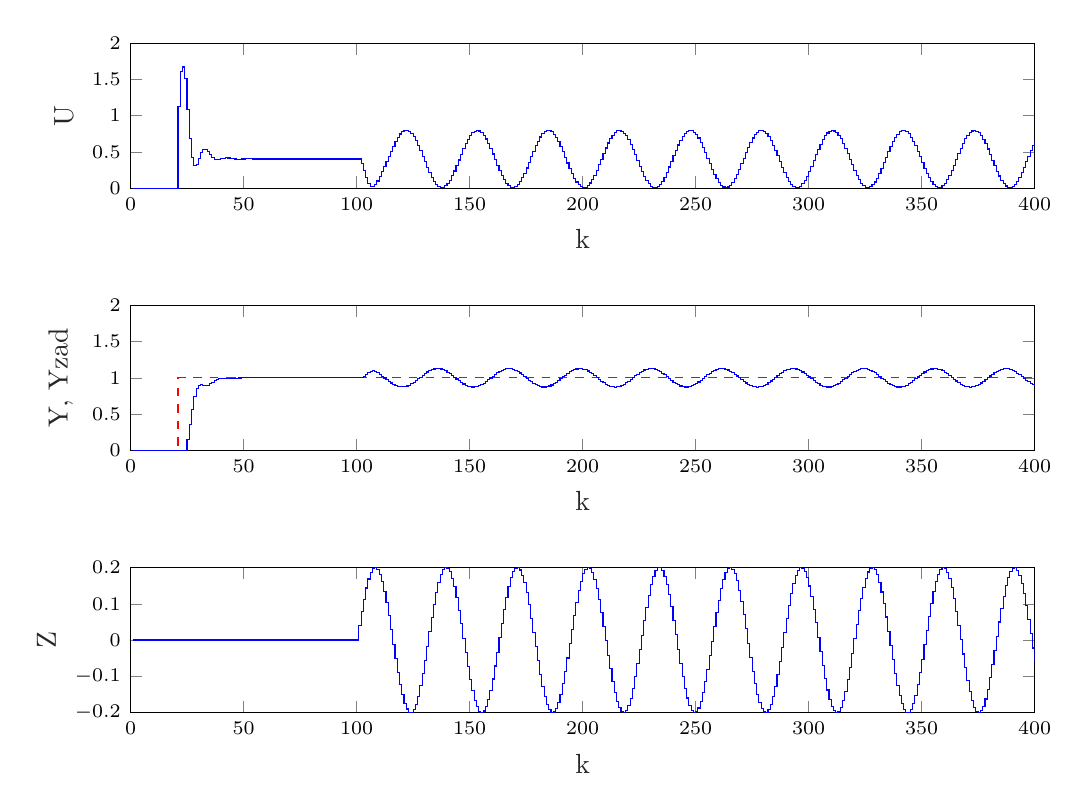
\begin{tikzpicture}

\begin{axis}[%
width=4.521in,
height=0.725in,
at={(0.758in,3.322in)},
scale only axis,
xmin=0,
xmax=400,
xlabel style={font=\color{white!15!black}},
xlabel={k},
ymin=0,
ymax=2,
ylabel style={font=\color{white!15!black}},
ylabel={U},
axis background/.style={fill=white}
]
\addplot[const plot, color=blue, forget plot] table[row sep=crcr] {%
1	0\\
2	0\\
3	0\\
4	0\\
5	0\\
6	0\\
7	0\\
8	0\\
9	0\\
10	0\\
11	0\\
12	0\\
13	0\\
14	0\\
15	0\\
16	0\\
17	0\\
18	0\\
19	0\\
20	0\\
21	1.13124041331753\\
22	1.60739620208848\\
23	1.67029772812697\\
24	1.5088290696095\\
25	1.08258009935487\\
26	0.684037120257817\\
27	0.424015380122655\\
28	0.310055013493176\\
29	0.329911659559614\\
30	0.412055543717462\\
31	0.49284813281035\\
32	0.53826796688865\\
33	0.537912993315766\\
34	0.504308140292631\\
35	0.45877281065022\\
36	0.419410565589577\\
37	0.396275443971251\\
38	0.390196587205243\\
39	0.395737940223536\\
40	0.405530115035693\\
41	0.413556147410279\\
42	0.416831988264799\\
43	0.415363749413303\\
44	0.41100616794113\\
45	0.406084453780792\\
46	0.402349250225408\\
47	0.40052789855623\\
48	0.400422166673599\\
49	0.401311205757422\\
50	0.402400609633999\\
51	0.403135629315426\\
52	0.403312371317209\\
53	0.403020350347085\\
54	0.402499132197402\\
55	0.401993011482922\\
56	0.401657765772953\\
57	0.40153450897489\\
58	0.401575545994931\\
59	0.40169360029823\\
60	0.40180770201165\\
61	0.401870068243431\\
62	0.401871046600647\\
63	0.40182832958733\\
64	0.401770153994924\\
65	0.401720848379131\\
66	0.401693163682481\\
67	0.401687705971358\\
68	0.401697066358232\\
69	0.40171140175517\\
70	0.401722879568028\\
71	0.401727766843836\\
72	0.401726257840868\\
73	0.401720930851284\\
74	0.401714902237765\\
75	0.401710465406525\\
76	0.401708535593691\\
77	0.401708807856827\\
78	0.40171030785626\\
79	0.401711988442695\\
80	0.401713135670161\\
81	0.401713504677854\\
82	0.401713234372025\\
83	0.401712653194794\\
84	0.401712087119452\\
85	0.401711739451988\\
86	0.401711660141687\\
87	0.401711782952107\\
88	0.401711991877851\\
89	0.401712181631659\\
90	0.401712292121399\\
91	0.40171231376668\\
92	0.401712272378503\\
93	0.401712206636815\\
94	0.401712149141236\\
95	0.401712116674031\\
96	0.401712109863984\\
97	0.401712118919425\\
98	0.401712131093258\\
99	0.401712136499113\\
100	0.401712130744792\\
101	0.401712114581669\\
102	0.334235295364013\\
103	0.2390343889258\\
104	0.143935098022229\\
105	0.0662976248260884\\
106	0.0255747278831896\\
107	0.0227085536006074\\
108	0.0503631547944995\\
109	0.0991979273976707\\
110	0.159444836804326\\
111	0.224891277756517\\
112	0.292813223027465\\
113	0.362441718882142\\
114	0.433642449231152\\
115	0.505562759706866\\
116	0.576108472576573\\
117	0.642174627887164\\
118	0.700215593912494\\
119	0.746920992479067\\
120	0.779723885135827\\
121	0.797031795494936\\
122	0.798224823517292\\
123	0.783510614938869\\
124	0.753742233375495\\
125	0.710272563829294\\
126	0.654867854582507\\
127	0.58966678082823\\
128	0.517152990292335\\
129	0.440110251554892\\
130	0.361543366322557\\
131	0.28456433264335\\
132	0.212255505643744\\
133	0.147526709075593\\
134	0.0929819233198008\\
135	0.0508061733855565\\
136	0.0226775599909048\\
137	0.00970511872147983\\
138	0.0123911417639461\\
139	0.0306163846595809\\
140	0.0636472807968308\\
141	0.110164968976698\\
142	0.168316022288995\\
143	0.235784119868662\\
144	0.309880741948237\\
145	0.387651658828556\\
146	0.465994863480688\\
147	0.541784868581303\\
148	0.611998000911901\\
149	0.673833415763506\\
150	0.724824910136951\\
151	0.76293913322666\\
152	0.786656411048066\\
153	0.795031094710474\\
154	0.787729109409936\\
155	0.765041228752116\\
156	0.727871519925772\\
157	0.677701374692524\\
158	0.6165305182971\\
159	0.546797323987093\\
160	0.47128160592513\\
161	0.392993775971781\\
162	0.315054798670057\\
163	0.240571743255718\\
164	0.172513900767026\\
165	0.113594405337491\\
166	0.0661620751216979\\
167	0.0321077796568143\\
168	0.0127890624508853\\
169	0.00897602199317402\\
170	0.020820608935247\\
171	0.0478505648888333\\
172	0.088988246151833\\
173	0.14259358312961\\
174	0.206529463264589\\
175	0.278246930688012\\
176	0.354886805430513\\
177	0.433393670401413\\
178	0.510637681463889\\
179	0.583539344299978\\
180	0.649192283683627\\
181	0.704979110913078\\
182	0.748675770303983\\
183	0.778540204881413\\
184	0.793381806471504\\
185	0.792608881398111\\
186	0.776252239413078\\
187	0.744963965386782\\
188	0.699991422695134\\
189	0.643127524700198\\
190	0.576639256856359\\
191	0.503177299059485\\
192	0.425670351326792\\
193	0.347208375716671\\
194	0.270919409263848\\
195	0.19984485900324\\
196	0.136818250668902\\
197	0.0843522649689548\\
198	0.0445385649409795\\
199	0.0189644079550476\\
200	0.00864936678234701\\
201	0.0140046824626434\\
202	0.0348168694448468\\
203	0.0702562266124021\\
204	0.118909914885383\\
205	0.178838282698892\\
206	0.247652193837894\\
207	0.32260827481125\\
208	0.400718284552564\\
209	0.478868246223199\\
210	0.553942591708697\\
211	0.622948369559626\\
212	0.683134564598481\\
213	0.732101772296593\\
214	0.767897855549882\\
215	0.789095770319742\\
216	0.794850457476509\\
217	0.784932513000496\\
218	0.759737271286672\\
219	0.720268949246041\\
220	0.668100859560196\\
221	0.605312757395917\\
222	0.534407921097868\\
223	0.458210510739775\\
224	0.379758991886682\\
225	0.302182596493468\\
226	0.228575357740125\\
227	0.161873214520335\\
228	0.104735471037573\\
229	0.0594390395911265\\
230	0.0277884046652801\\
231	0.0110440870673605\\
232	0.00987295215752237\\
233	0.0243217517293651\\
234	0.0538150234321128\\
235	0.0971777140479765\\
236	0.152681693225108\\
237	0.218114461841866\\
238	0.290867358364439\\
239	0.368039678694765\\
240	0.446554485881807\\
241	0.523281414217985\\
242	0.595161526893795\\
243	0.659329251313597\\
244	0.713226558419802\\
245	0.754704871631463\\
246	0.782110672883595\\
247	0.794351405534735\\
248	0.790939043088506\\
249	0.772009573099859\\
250	0.738317604062009\\
251	0.691206299608933\\
252	0.632553835215928\\
253	0.564698514765994\\
254	0.490345538308765\\
255	0.412459143759277\\
256	0.334144426120043\\
257	0.258523546460307\\
258	0.188611264335441\\
259	0.127194753366711\\
260	0.0767224892180033\\
261	0.0392066384976454\\
262	0.0161428399609795\\
263	0.00845057676541253\\
264	0.0164365178775388\\
265	0.0397822908440518\\
266	0.0775571737384079\\
267	0.128255200251305\\
268	0.189855198372299\\
269	0.259901368764616\\
270	0.335601190173868\\
271	0.413936748591808\\
272	0.4917850518725\\
273	0.566042533353708\\
274	0.633748781041464\\
275	0.69220455974909\\
276	0.739079421045906\\
277	0.77250461092451\\
278	0.79114757120594\\
279	0.794265064503145\\
280	0.781732804791574\\
281	0.75405041230407\\
282	0.712321495224436\\
283	0.658209652276577\\
284	0.593872150262119\\
285	0.521873920621949\\
286	0.445085303708022\\
287	0.366567617374191\\
288	0.289451111899039\\
289	0.216810176787778\\
290	0.151540774561792\\
291	0.0962449878640206\\
292	0.0531272826245305\\
293	0.0239066229486957\\
294	0.00974794143166188\\
295	0.0112156969620783\\
296	0.0282513715186682\\
297	0.0601758030966688\\
298	0.105716262945111\\
299	0.163057200168537\\
300	0.229912632429163\\
301	0.303617276120156\\
302	0.381232793290691\\
303	0.459664925247105\\
304	0.535787009633834\\
305	0.606564431000964\\
306	0.669175540633437\\
307	0.721124161112345\\
308	0.760339093189237\\
309	0.785256773125997\\
310	0.794883679886671\\
311	0.788835972179991\\
312	0.767354792390088\\
313	0.731296617089881\\
314	0.682099065180771\\
315	0.621723550302131\\
316	0.55257707060558\\
317	0.477416255926487\\
318	0.39923748936748\\
319	0.32115747209571\\
320	0.246288984790514\\
321	0.177616795072957\\
322	0.11787865947241\\
323	0.0694561685167154\\
324	0.034279791350528\\
325	0.013751908682509\\
326	0.00869090341773893\\
327	0.0192985368458738\\
328	0.0451519089936488\\
329	0.085220321754142\\
330	0.13790637139168\\
331	0.201109632034122\\
332	0.272310391846315\\
333	0.348670104419918\\
334	0.427144551410107\\
335	0.504605205343635\\
336	0.57796395423722\\
337	0.644296215393767\\
338	0.700957529891402\\
339	0.745688989258491\\
340	0.776707291196853\\
341	0.792775834143517\\
342	0.793254016464086\\
343	0.778122774997156\\
344	0.747985344894957\\
345	0.704043210497858\\
346	0.648048205987048\\
347	0.582232675367318\\
348	0.509220476036542\\
349	0.431922373920278\\
350	0.353420000430134\\
351	0.276842997525196\\
352	0.20524424873227\\
353	0.141478170286089\\
354	0.0880869145467008\\
355	0.0471990224060222\\
356	0.0204445650879757\\
357	0.00889015836454157\\
358	0.0129964399604433\\
359	0.0325997053853986\\
360	0.0669184343153632\\
361	0.114584447338314\\
362	0.173697450945774\\
363	0.241900796235197\\
364	0.316475431063621\\
365	0.394448300076565\\
366	0.472710871044376\\
367	0.548143062234197\\
368	0.617737630223725\\
369	0.678720059206948\\
370	0.728659172183642\\
371	0.765564054313876\\
372	0.78796342440949\\
373	0.794964290271864\\
374	0.786287549472819\\
375	0.762279116287779\\
376	0.723896131185407\\
377	0.672668802657736\\
378	0.610639402636554\\
379	0.540280847556268\\
380	0.46439811097937\\
381	0.386016398152041\\
382	0.308260540617524\\
383	0.234230419043448\\
384	0.166877380761845\\
385	0.108886578864567\\
386	0.0625699236230218\\
387	0.0297739139213382\\
388	0.0118060231728269\\
389	0.00938257448095886\\
390	0.0226001830977192\\
391	0.050931904678384\\
392	0.0932482428896748\\
393	0.14786217886423\\
394	0.212596427319152\\
395	0.284870238049415\\
396	0.36180228229452\\
397	0.44032552222361\\
398	0.51730948405519\\
399	0.589685060168019\\
400	0.654566864736822\\
};
\end{axis}

\begin{axis}[%
width=4.521in,
height=0.725in,
at={(0.758in,2.011in)},
scale only axis,
xmin=0,
xmax=400,
xlabel style={font=\color{white!15!black}},
xlabel={k},
ymin=0,
ymax=2,
ylabel style={font=\color{white!15!black}},
ylabel={Y, Yzad},
axis background/.style={fill=white}
]
\addplot[const plot, color=red, dashed, forget plot] table[row sep=crcr] {%
1	0\\
2	0\\
3	0\\
4	0\\
5	0\\
6	0\\
7	0\\
8	0\\
9	0\\
10	0\\
11	0\\
12	0\\
13	0\\
14	0\\
15	0\\
16	0\\
17	0\\
18	0\\
19	0\\
20	0\\
21	1\\
22	1\\
23	1\\
24	1\\
25	1\\
26	1\\
27	1\\
28	1\\
29	1\\
30	1\\
31	1\\
32	1\\
33	1\\
34	1\\
35	1\\
36	1\\
37	1\\
38	1\\
39	1\\
40	1\\
41	1\\
42	1\\
43	1\\
44	1\\
45	1\\
46	1\\
47	1\\
48	1\\
49	1\\
50	1\\
51	1\\
52	1\\
53	1\\
54	1\\
55	1\\
56	1\\
57	1\\
58	1\\
59	1\\
60	1\\
61	1\\
62	1\\
63	1\\
64	1\\
65	1\\
66	1\\
67	1\\
68	1\\
69	1\\
70	1\\
71	1\\
72	1\\
73	1\\
74	1\\
75	1\\
76	1\\
77	1\\
78	1\\
79	1\\
80	1\\
81	1\\
82	1\\
83	1\\
84	1\\
85	1\\
86	1\\
87	1\\
88	1\\
89	1\\
90	1\\
91	1\\
92	1\\
93	1\\
94	1\\
95	1\\
96	1\\
97	1\\
98	1\\
99	1\\
100	1\\
101	1\\
102	1\\
103	1\\
104	1\\
105	1\\
106	1\\
107	1\\
108	1\\
109	1\\
110	1\\
111	1\\
112	1\\
113	1\\
114	1\\
115	1\\
116	1\\
117	1\\
118	1\\
119	1\\
120	1\\
121	1\\
122	1\\
123	1\\
124	1\\
125	1\\
126	1\\
127	1\\
128	1\\
129	1\\
130	1\\
131	1\\
132	1\\
133	1\\
134	1\\
135	1\\
136	1\\
137	1\\
138	1\\
139	1\\
140	1\\
141	1\\
142	1\\
143	1\\
144	1\\
145	1\\
146	1\\
147	1\\
148	1\\
149	1\\
150	1\\
151	1\\
152	1\\
153	1\\
154	1\\
155	1\\
156	1\\
157	1\\
158	1\\
159	1\\
160	1\\
161	1\\
162	1\\
163	1\\
164	1\\
165	1\\
166	1\\
167	1\\
168	1\\
169	1\\
170	1\\
171	1\\
172	1\\
173	1\\
174	1\\
175	1\\
176	1\\
177	1\\
178	1\\
179	1\\
180	1\\
181	1\\
182	1\\
183	1\\
184	1\\
185	1\\
186	1\\
187	1\\
188	1\\
189	1\\
190	1\\
191	1\\
192	1\\
193	1\\
194	1\\
195	1\\
196	1\\
197	1\\
198	1\\
199	1\\
200	1\\
201	1\\
202	1\\
203	1\\
204	1\\
205	1\\
206	1\\
207	1\\
208	1\\
209	1\\
210	1\\
211	1\\
212	1\\
213	1\\
214	1\\
215	1\\
216	1\\
217	1\\
218	1\\
219	1\\
220	1\\
221	1\\
222	1\\
223	1\\
224	1\\
225	1\\
226	1\\
227	1\\
228	1\\
229	1\\
230	1\\
231	1\\
232	1\\
233	1\\
234	1\\
235	1\\
236	1\\
237	1\\
238	1\\
239	1\\
240	1\\
241	1\\
242	1\\
243	1\\
244	1\\
245	1\\
246	1\\
247	1\\
248	1\\
249	1\\
250	1\\
251	1\\
252	1\\
253	1\\
254	1\\
255	1\\
256	1\\
257	1\\
258	1\\
259	1\\
260	1\\
261	1\\
262	1\\
263	1\\
264	1\\
265	1\\
266	1\\
267	1\\
268	1\\
269	1\\
270	1\\
271	1\\
272	1\\
273	1\\
274	1\\
275	1\\
276	1\\
277	1\\
278	1\\
279	1\\
280	1\\
281	1\\
282	1\\
283	1\\
284	1\\
285	1\\
286	1\\
287	1\\
288	1\\
289	1\\
290	1\\
291	1\\
292	1\\
293	1\\
294	1\\
295	1\\
296	1\\
297	1\\
298	1\\
299	1\\
300	1\\
301	1\\
302	1\\
303	1\\
304	1\\
305	1\\
306	1\\
307	1\\
308	1\\
309	1\\
310	1\\
311	1\\
312	1\\
313	1\\
314	1\\
315	1\\
316	1\\
317	1\\
318	1\\
319	1\\
320	1\\
321	1\\
322	1\\
323	1\\
324	1\\
325	1\\
326	1\\
327	1\\
328	1\\
329	1\\
330	1\\
331	1\\
332	1\\
333	1\\
334	1\\
335	1\\
336	1\\
337	1\\
338	1\\
339	1\\
340	1\\
341	1\\
342	1\\
343	1\\
344	1\\
345	1\\
346	1\\
347	1\\
348	1\\
349	1\\
350	1\\
351	1\\
352	1\\
353	1\\
354	1\\
355	1\\
356	1\\
357	1\\
358	1\\
359	1\\
360	1\\
361	1\\
362	1\\
363	1\\
364	1\\
365	1\\
366	1\\
367	1\\
368	1\\
369	1\\
370	1\\
371	1\\
372	1\\
373	1\\
374	1\\
375	1\\
376	1\\
377	1\\
378	1\\
379	1\\
380	1\\
381	1\\
382	1\\
383	1\\
384	1\\
385	1\\
386	1\\
387	1\\
388	1\\
389	1\\
390	1\\
391	1\\
392	1\\
393	1\\
394	1\\
395	1\\
396	1\\
397	1\\
398	1\\
399	1\\
400	1\\
};
\addplot[const plot, color=blue, forget plot] table[row sep=crcr] {%
1	0\\
2	0\\
3	0\\
4	0\\
5	0\\
6	0\\
7	0\\
8	0\\
9	0\\
10	0\\
11	0\\
12	0\\
13	0\\
14	0\\
15	0\\
16	0\\
17	0\\
18	0\\
19	0\\
20	0\\
21	0\\
22	0\\
23	0\\
24	0\\
25	0.152830579839198\\
26	0.361723685979986\\
27	0.567813252929803\\
28	0.740934525440941\\
29	0.847095360437015\\
30	0.893658115143514\\
31	0.90255973864811\\
32	0.895570671873684\\
33	0.89163036498361\\
34	0.898990405246294\\
35	0.91685828271975\\
36	0.939887677878803\\
37	0.961615803129477\\
38	0.977621370527924\\
39	0.986602460199098\\
40	0.989773437013205\\
41	0.989641380644215\\
42	0.988689847199495\\
43	0.988533654813312\\
44	0.989704626042417\\
45	0.991892848316057\\
46	0.994401945347177\\
47	0.996573965969035\\
48	0.998037076898529\\
49	0.998753666950623\\
50	0.998924656597726\\
51	0.998838350857697\\
52	0.998740665168325\\
53	0.998766808279368\\
54	0.998937329483177\\
55	0.999196697549384\\
56	0.999464818354491\\
57	0.999678006297738\\
58	0.999808372281484\\
59	0.999862529279366\\
60	0.999867769339971\\
61	0.999855454910885\\
62	0.999848800913543\\
63	0.999857968169211\\
64	0.999881621834702\\
65	0.999912037309881\\
66	0.999940598025195\\
67	0.999961538784302\\
68	0.999973216807206\\
69	0.999977361349574\\
70	0.999977327623101\\
71	0.999976368399375\\
72	0.999976556980123\\
73	0.999978522354457\\
74	0.999981799158156\\
75	0.999985440953475\\
76	0.999988577040411\\
77	0.999990730653257\\
78	0.99999187053213\\
79	0.999992275801492\\
80	0.999992333120867\\
81	0.99999236613075\\
82	0.999992548519416\\
83	0.999992902381439\\
84	0.999993351510946\\
85	0.999993790164412\\
86	0.999994136571704\\
87	0.999994357305398\\
88	0.999994464385011\\
89	0.999994496292151\\
90	0.999994495860299\\
91	0.999994494377281\\
92	0.999994505516522\\
93	0.999994527765157\\
94	0.999994551375948\\
95	0.999994565659013\\
96	0.999994563834085\\
97	0.999994544575335\\
98	0.999994510910527\\
99	0.999994467862375\\
100	0.999994420170427\\
101	0.999994370909295\\
102	1.00846756814737\\
103	1.02412524042148\\
104	1.04549873740651\\
105	1.07098615417743\\
106	1.0897894869801\\
107	1.09695204608207\\
108	1.09148974686446\\
109	1.07482345376639\\
110	1.05099280528335\\
111	1.0240726379727\\
112	0.997106822830562\\
113	0.971940429321492\\
114	0.949265271494161\\
115	0.929190730356925\\
116	0.911763172898169\\
117	0.897237902125641\\
118	0.886145599729037\\
119	0.879160275186301\\
120	0.876892346374106\\
121	0.879713998401527\\
122	0.887662570353424\\
123	0.900434028800379\\
124	0.917441234462095\\
125	0.937898460658789\\
126	0.960901757791112\\
127	0.98548850360104\\
128	1.0106745836872\\
129	1.03547746195109\\
130	1.05893570747977\\
131	1.08013275997311\\
132	1.09822753530338\\
133	1.11248968877153\\
134	1.12233470367997\\
135	1.12735367004439\\
136	1.12733400610924\\
137	1.1222694285396\\
138	1.11235929446379\\
139	1.09799855160112\\
140	1.07975990052392\\
141	1.05836963742826\\
142	1.0346783377447\\
143	1.00962731998219\\
144	0.984211811732718\\
145	0.959441906336624\\
146	0.936302648672162\\
147	0.915714805896407\\
148	0.898497980345131\\
149	0.885337675649939\\
150	0.876757747820665\\
151	0.87309940097526\\
152	0.87450756758343\\
153	0.880925180462769\\
154	0.892095518043524\\
155	0.907572492709888\\
156	0.926738455234154\\
157	0.948828807409089\\
158	0.972962454691947\\
159	0.998176900080328\\
160	1.02346659118666\\
161	1.04782299602912\\
162	1.07027480826367\\
163	1.0899266742636\\
164	1.10599489310515\\
165	1.11783866284971\\
166	1.12498562633376\\
167	1.12715069876355\\
168	1.12424742812056\\
169	1.11639143703251\\
170	1.10389580984113\\
171	1.08725860897402\\
172	1.06714301795446\\
173	1.04435090210635\\
174	1.01979084048842\\
175	0.994441903229234\\
176	0.969314618296533\\
177	0.945410683951149\\
178	0.923683033200544\\
179	0.90499784250252\\
180	0.890099999381749\\
181	0.879583405648838\\
182	0.873867300082941\\
183	0.87317954444952\\
184	0.877547539133908\\
185	0.886797130530064\\
186	0.900559553743016\\
187	0.918286133835661\\
188	0.939270159544737\\
189	0.962675057441526\\
190	0.987567743325218\\
191	1.01295582122954\\
192	1.03782714702727\\
193	1.06119017934828\\
194	1.08211350914147\\
195	1.09976299195905\\
196	1.11343500261617\\
197	1.12258448646869\\
198	1.12684668899436\\
199	1.12605169738803\\
200	1.12023121444303\\
201	1.10961729466431\\
202	1.09463309299939\\
203	1.07587599500484\\
204	1.05409380099472\\
205	1.03015491363343\\
206	1.00501371749964\\
207	0.979672530828834\\
208	0.955141646298545\\
209	0.93239905390413\\
210	0.912351451646891\\
211	0.89579809841531\\
212	0.883398950130936\\
213	0.875648349470253\\
214	0.872855318070408\\
215	0.8751312369065\\
216	0.882385405985153\\
217	0.894328660375589\\
218	0.910484898418745\\
219	0.930210062521374\\
220	0.952717815831076\\
221	0.977110888476762\\
222	1.00241683807791\\
223	1.02762679487319\\
224	1.05173569387671\\
225	1.07378236413806\\
226	1.09288786616339\\
227	1.10829016584793\\
228	1.11937498009483\\
229	1.12570038196096\\
230	1.1270143644332\\
231	1.12326489694906\\
232	1.11460180714353\\
233	1.10137066079897\\
234	1.08409894590141\\
235	1.06347506064144\\
236	1.04032096132319\\
237	1.01555949800297\\
238	0.990177690182373\\
239	0.965187397611719\\
240	0.941584954854863\\
241	0.920311400957579\\
242	0.902214916390749\\
243	0.888016980815316\\
244	0.878283606190112\\
245	0.87340278650983\\
246	0.873569051841418\\
247	0.878775731955199\\
248	0.888815231775185\\
249	0.90328730687906\\
250	0.921615012474442\\
251	0.943067694883721\\
252	0.966790113042385\\
253	0.991836531061098\\
254	1.01720842252499\\
255	1.04189428178203\\
256	1.06490995309411\\
257	1.08533786835933\\
258	1.10236362851188\\
259	1.11530847043164\\
260	1.12365632570349\\
261	1.12707439323494\\
262	1.12542640608237\\
263	1.11877806374181\\
264	1.10739441320076\\
265	1.09172928287598\\
266	1.07240719039432\\
267	1.05019844532511\\
268	1.02598843940275\\
269	1.00074234860858\\
270	0.975466654438754\\
271	0.951169018482647\\
272	0.92881811003964\\
273	0.909304988325098\\
274	0.893407578805095\\
275	0.88175965983456\\
276	0.874825595969611\\
277	0.872881825240674\\
278	0.876005838431606\\
279	0.884073089738624\\
280	0.896761961986487\\
281	0.913566588465848\\
282	0.933817020230242\\
283	0.956705934844739\\
284	0.981320821787769\\
285	1.00668036137025\\
286	1.03177354685556\\
287	1.05559999010362\\
288	1.07720980388108\\
289	1.09574147085762\\
290	1.11045618957281\\
291	1.12076732810955\\
292	1.12626381124908\\
293	1.12672650873526\\
294	1.12213697129903\\
295	1.11267816616442\\
296	1.09872718271368\\
297	1.08084019911341\\
298	1.05973030923506\\
299	1.0362390938407\\
300	1.01130306940141\\
301	0.985916352128886\\
302	0.961091025848729\\
303	0.937816794218676\\
304	0.917021526537232\\
305	0.899534267936835\\
306	0.886052188021748\\
307	0.877112785794239\\
308	0.873072481651674\\
309	0.874092400348387\\
310	0.880131931991292\\
311	0.890950338331847\\
312	0.906116337171324\\
313	0.925025295364656\\
314	0.946923342667026\\
315	0.970937438554292\\
316	0.996110189504144\\
317	1.02143802367071\\
318	1.04591119986754\\
319	1.06855405788774\\
320	1.08846390837952\\
321	1.10484701485248\\
322	1.11705023503116\\
323	1.12458706014706\\
324	1.12715701300522\\
325	1.12465762998774\\
326	1.11718854807855\\
327	1.10504753341758\\
328	1.08871860982925\\
329	1.06885276114891\\
330	1.04624197732578\\
331	1.02178767946545\\
332	0.996464782773813\\
333	0.971282830001139\\
334	0.947245744628957\\
335	0.925311808060194\\
336	0.906355456231456\\
337	0.891132418652912\\
338	0.880249589727547\\
339	0.874140833586369\\
340	0.873049687118955\\
341	0.87701965082978\\
342	0.885892454601059\\
343	0.899314367473909\\
344	0.916750299856761\\
345	0.937505135916384\\
346	0.960751445678871\\
347	0.985562472046567\\
348	1.01094907765433\\
349	1.03589917862562\\
350	1.05941809314088\\
351	1.08056819625322\\
352	1.098506300038\\
353	1.11251726884294\\
354	1.12204252949913\\
355	1.12670233987682\\
356	1.12631092800755\\
357	1.12088389822417\\
358	1.11063760906137\\
359	1.09598054771972\\
360	1.07749704496748\\
361	1.05592397971601\\
362	1.03212140198339\\
363	1.00703824541545\\
364	0.981674496296792\\
365	0.957041327253833\\
366	0.934120784993076\\
367	0.913826639197481\\
368	0.896967953412166\\
369	0.884216830233491\\
370	0.876081616699184\\
371	0.872886638096041\\
372	0.874759268134281\\
373	0.881624850959779\\
374	0.893209677447466\\
375	0.909051897120418\\
376	0.928519930670865\\
377	0.950837649034038\\
378	0.975115315204665\\
379	1.00038505524357\\
380	1.02563944435729\\
381	1.04987166974545\\
382	1.07211566904993\\
383	1.09148464421251\\
384	1.107206415315\\
385	1.11865420495579\\
386	1.12537162588696\\
387	1.12709087573358\\
388	1.12374341342932\\
389	1.11546269173243\\
390	1.10257883688542\\
391	1.0856054875235\\
392	1.06521931752312\\
393	1.04223305914983\\
394	1.01756310198761\\
395	0.992192959377957\\
396	0.967134058846649\\
397	0.943385419679988\\
398	0.921893825178462\\
399	0.903516077394291\\
400	0.888984839137397\\
};
\end{axis}

\begin{axis}[%
width=4.521in,
height=0.725in,
at={(0.758in,0.7in)},
scale only axis,
xmin=0,
xmax=400,
xlabel style={font=\color{white!15!black}},
xlabel={k},
ymin=-0.2,
ymax=0.2,
ylabel style={font=\color{white!15!black}},
ylabel={Z},
axis background/.style={fill=white}
]
\addplot[const plot, color=blue, forget plot] table[row sep=crcr] {%
1	0\\
2	0\\
3	0\\
4	0\\
5	0\\
6	0\\
7	0\\
8	0\\
9	0\\
10	0\\
11	0\\
12	0\\
13	0\\
14	0\\
15	0\\
16	0\\
17	0\\
18	0\\
19	0\\
20	0\\
21	0\\
22	0\\
23	0\\
24	0\\
25	0\\
26	0\\
27	0\\
28	0\\
29	0\\
30	0\\
31	0\\
32	0\\
33	0\\
34	0\\
35	0\\
36	0\\
37	0\\
38	0\\
39	0\\
40	0\\
41	0\\
42	0\\
43	0\\
44	0\\
45	0\\
46	0\\
47	0\\
48	0\\
49	0\\
50	0\\
51	0\\
52	0\\
53	0\\
54	0\\
55	0\\
56	0\\
57	0\\
58	0\\
59	0\\
60	0\\
61	0\\
62	0\\
63	0\\
64	0\\
65	0\\
66	0\\
67	0\\
68	0\\
69	0\\
70	0\\
71	0\\
72	0\\
73	0\\
74	0\\
75	0\\
76	0\\
77	0\\
78	0\\
79	0\\
80	0\\
81	0\\
82	0\\
83	0\\
84	0\\
85	0\\
86	0\\
87	0\\
88	0\\
89	0\\
90	0\\
91	0\\
92	0\\
93	0\\
94	0\\
95	0\\
96	0\\
97	0\\
98	0\\
99	0\\
100	0\\
101	0.0397338661590122\\
102	0.0778836684617301\\
103	0.112928494679007\\
104	0.143471218179905\\
105	0.168294196961579\\
106	0.186407817193445\\
107	0.197089945997692\\
108	0.199914720608301\\
109	0.194769526175639\\
110	0.181859485365136\\
111	0.161699280763918\\
112	0.13509263611023\\
113	0.103100274364293\\
114	0.0669976300311809\\
115	0.0282240016119734\\
116	-0.011674828685516\\
117	-0.0511082204053663\\
118	-0.0885040886589705\\
119	-0.122371578188544\\
120	-0.151360499061586\\
121	-0.174315154482718\\
122	-0.190320414777903\\
123	-0.198738200726693\\
124	-0.199232921767168\\
125	-0.191784854932628\\
126	-0.176690931144031\\
127	-0.154552897511197\\
128	-0.126253327574464\\
129	-0.0929204358827513\\
130	-0.0558830996397852\\
131	-0.0166178805634993\\
132	0.0233098409700987\\
133	0.0623082727026757\\
134	0.0988226702277218\\
135	0.131397319743758\\
136	0.158733572769831\\
137	0.179741619162325\\
138	0.193583934406297\\
139	0.199708669074921\\
140	0.197871649324676\\
141	0.188146111335955\\
142	0.170919781617656\\
143	0.146879419574823\\
144	0.116983438578352\\
145	0.0824236970483513\\
146	0.0445779828200492\\
147	0.00495508509067155\\
148	-0.0348653562445963\\
149	-0.0732958258503857\\
150	-0.108804222177874\\
151	-0.139974937518709\\
152	-0.165565293817131\\
153	-0.184555084322561\\
154	-0.196187246013298\\
155	-0.199998041310141\\
156	-0.195835545830263\\
157	-0.183865705132935\\
158	-0.164565718993742\\
159	-0.138705016955424\\
160	-0.107314583600087\\
161	-0.0716458564473654\\
162	-0.0331208350896619\\
163	0.00672460944422769\\
164	0.0463019650203078\\
165	0.0840334073653282\\
166	0.118414702941445\\
167	0.14807517799049\\
168	0.171832362971299\\
169	0.188739133888821\\
170	0.198121471138974\\
171	0.199605330543272\\
172	0.193131555309855\\
173	0.178958234428101\\
174	0.157650413475063\\
175	0.130057568031423\\
176	0.0972797377707596\\
177	0.0606236713491405\\
178	0.0215507304598885\\
179	-0.0183813700455363\\
180	-0.0575806633330131\\
181	-0.0944843972796932\\
182	-0.12762133646959\\
183	-0.15567041570686\\
184	-0.177513406716301\\
185	-0.192279498375911\\
186	-0.199380013208319\\
187	-0.198531876094127\\
188	-0.189768899583625\\
189	-0.173440435897116\\
190	-0.150197449354335\\
191	-0.120966564481257\\
192	-0.0869131244143787\\
193	-0.0493947323473242\\
194	-0.00990712817567348\\
195	0.0299754419325905\\
196	0.0686629857639798\\
197	0.10461315303154\\
198	0.136392724013627\\
199	0.162734747501421\\
200	0.182589050145526\\
201	0.195164103553395\\
202	0.199958580028534\\
203	0.196781338923723\\
204	0.185759046815448\\
205	0.167331127707211\\
206	0.142232244581196\\
207	0.111463010703532\\
208	0.076250098330988\\
209	0.0379973351590875\\
210	-0.00177026185808078\\
211	-0.0414672841213524\\
212	-0.0795111366242872\\
213	-0.114385131021913\\
214	-0.144698951208849\\
215	-0.169244080835034\\
216	-0.187041983038908\\
217	-0.19738311162413\\
218	-0.199855198427326\\
219	-0.194359689148773\\
220	-0.181115672401325\\
221	-0.160651145338791\\
222	-0.133781964075604\\
223	-0.101579318078124\\
224	-0.0653270252209445\\
225	-0.0264703500195546\\
226	0.0134416145050957\\
227	0.0528177042768946\\
228	0.0900881188550779\\
229	0.123767004424008\\
230	0.152511690095921\\
231	0.175176215962178\\
232	0.19085701889854\\
233	0.198928954775568\\
234	0.199070220982312\\
235	0.191275185680901\\
236	0.175854612330145\\
237	0.153423270527106\\
238	0.124875427083278\\
239	0.0913491944288386\\
240	0.0541811576615738\\
241	0.0148530891168716\\
242	-0.0250671252192865\\
243	-0.0639879923768396\\
244	-0.100357860204115\\
245	-0.132726776842594\\
246	-0.159804295731923\\
247	-0.180510921642037\\
248	-0.194021146741437\\
249	-0.19979636098939\\
250	-0.197606324818572\\
251	-0.187538348060056\\
252	-0.169993809175866\\
253	-0.145672153566319\\
254	-0.115543008889147\\
255	-0.080807529064613\\
256	-0.0428505080591775\\
257	-0.00318517252002036\\
258	0.0366071457961169\\
259	0.0749400527298918\\
260	0.110285336248338\\
261	0.141233891436067\\
262	0.166551897061556\\
263	0.185230004136105\\
264	0.196523575472828\\
265	0.199982372021453\\
266	0.195468502478452\\
267	0.183161920578164\\
268	0.163553250905289\\
269	0.137424229240949\\
270	0.105816537224005\\
271	0.0699902737913324\\
272	0.031373719009682\\
273	-0.00849360694338889\\
274	-0.0480223195907549\\
275	-0.0856365338992302\\
276	-0.119836689842853\\
277	-0.149259335128983\\
278	-0.17273148173859\\
279	-0.189317369256992\\
280	-0.198355770688623\\
281	-0.19948635349073\\
282	-0.192664044894752\\
283	-0.178160828815373\\
284	-0.156554902710131\\
285	-0.1287076266714\\
286	-0.095729183717683\\
287	-0.0589343203000515\\
288	-0.0197899315100593\\
289	0.0201434193985001\\
290	0.0592737157418771\\
291	0.0960409560876518\\
292	0.128979346588973\\
293	0.156775737559658\\
294	0.178321974608288\\
295	0.192759077256818\\
296	0.199511483781561\\
297	0.198309997042828\\
298	0.189202516525382\\
299	0.172552128737136\\
300	0.14902263209587\\
301	0.119552073381051\\
302	0.0853153507689146\\
303	0.0476773743497798\\
304	0.00813865146997297\\
305	-0.0317245337609418\\
306	-0.0703229619433633\\
307	-0.106117835550041\\
308	-0.137682125927533\\
309	-0.163757464425369\\
310	-0.183304309583127\\
311	-0.195543390368004\\
312	-0.199986773251761\\
313	-0.196457314580727\\
314	-0.185095722734266\\
315	-0.16635494852572\\
316	-0.14098212748285\\
317	-0.10998879391207\\
318	-0.0746105542177258\\
319	-0.036257827173939\\
320	0.00354038502108272\\
321	0.0431974532376448\\
322	0.0811323753110672\\
323	0.115832805608854\\
324	0.145915347478571\\
325	0.170180704906824\\
326	0.187661494666711\\
327	0.197660812834327\\
328	0.199780018149004\\
329	0.193934624582384\\
330	0.180357669529762\\
331	0.159590423344526\\
332	0.132460810597249\\
333	0.100050403335717\\
334	0.0636513022204976\\
335	0.0247146245490448\\
336	-0.0152073472116707\\
337	-0.0545230500286148\\
338	-0.0916650908983532\\
339	-0.125152733859895\\
340	-0.153650932264733\\
341	-0.176023552873732\\
342	-0.191378669904098\\
343	-0.199104123295703\\
344	-0.198891923600903\\
345	-0.190750530551894\\
346	-0.175004515797889\\
347	-0.152281623257708\\
348	-0.123487742950692\\
349	-0.0897707960203409\\
350	-0.0524749707407858\\
351	-0.0130871339721414\\
352	0.0268224455291314\\
353	0.0656626987702807\\
354	0.101885187422086\\
355	0.134045835168675\\
356	0.160862498473183\\
357	0.181266081594533\\
358	0.194443158060908\\
359	0.199868399416262\\
360	0.197325518408097\\
361	0.186915891677683\\
362	0.169054518193285\\
363	0.144453474550903\\
364	0.114093526727476\\
365	0.0791850300363668\\
366	0.0411196760805202\\
367	0.00141501039998619\\
368	-0.0383460672798732\\
369	-0.0765784082652954\\
370	-0.111757809770323\\
371	-0.142481780071971\\
372	-0.167525451429406\\
373	-0.185890411695483\\
374	-0.196844507858378\\
375	-0.199951034671724\\
376	-0.195086144714686\\
377	-0.182443785797804\\
378	-0.162527968875822\\
379	-0.136132674721426\\
380	-0.104310200417382\\
381	-0.0683292075925703\\
382	-0.0296241448863273\\
383	0.0102619389921399\\
384	0.0497389117464102\\
385	0.087232951049565\\
386	0.121249287873869\\
387	0.150431798214895\\
388	0.173617067476084\\
389	0.18988077213734\\
390	0.198574529616907\\
391	0.199351747238813\\
392	0.192181439789124\\
393	0.177349464798646\\
394	0.155447126305245\\
395	0.127347601427828\\
396	0.0941711295500773\\
397	0.0572403519113507\\
398	0.0180275820742931\\
399	-0.0219038905707402\\
400	-0.0609621242204433\\
};
\end{axis}
\end{tikzpicture}%
	\label{6przebieg}
\end{figure}

\subsection{Z uwzględnieniem zakłóceń}

W trybie pracy algorytmu z uwzględnianiem zakłóceń otrzymano wskaźnik jakości $e$~=~\num{7.8234}. Przebieg przedstawiono na rysunku \ref{6zprzebieg}

\begin{figure}
	
	\centering
	\caption{ Przebieg symulacji algorytmu DMC dla zakłócenia zmiennego sinusoidalnie z uwzględnianiem zakłóceń }
	% This file was created by matlab2tikz.
%
%The latest updates can be retrieved from
%  http://www.mathworks.com/matlabcentral/fileexchange/22022-matlab2tikz-matlab2tikz
%where you can also make suggestions and rate matlab2tikz.
%
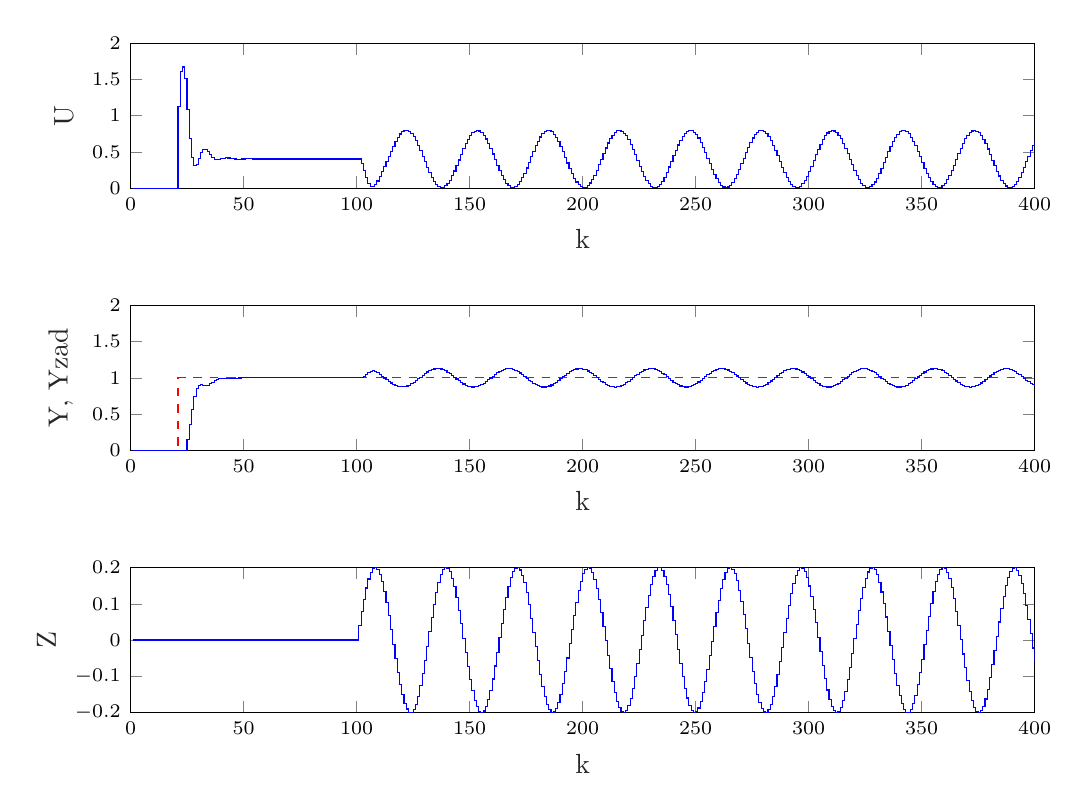
\begin{tikzpicture}

\begin{axis}[%
width=4.521in,
height=0.725in,
at={(0.758in,3.322in)},
scale only axis,
xmin=0,
xmax=400,
xlabel style={font=\color{white!15!black}},
xlabel={k},
ymin=0,
ymax=2,
ylabel style={font=\color{white!15!black}},
ylabel={U},
axis background/.style={fill=white}
]
\addplot[const plot, color=blue, forget plot] table[row sep=crcr] {%
1	0\\
2	0\\
3	0\\
4	0\\
5	0\\
6	0\\
7	0\\
8	0\\
9	0\\
10	0\\
11	0\\
12	0\\
13	0\\
14	0\\
15	0\\
16	0\\
17	0\\
18	0\\
19	0\\
20	0\\
21	1.13124041331753\\
22	1.60739620208848\\
23	1.67029772812697\\
24	1.5088290696095\\
25	1.08258009935487\\
26	0.684037120257817\\
27	0.424015380122655\\
28	0.310055013493176\\
29	0.329911659559614\\
30	0.412055543717462\\
31	0.49284813281035\\
32	0.53826796688865\\
33	0.537912993315766\\
34	0.504308140292631\\
35	0.45877281065022\\
36	0.419410565589577\\
37	0.396275443971251\\
38	0.390196587205243\\
39	0.395737940223536\\
40	0.405530115035693\\
41	0.413556147410279\\
42	0.416831988264799\\
43	0.415363749413303\\
44	0.41100616794113\\
45	0.406084453780792\\
46	0.402349250225408\\
47	0.40052789855623\\
48	0.400422166673599\\
49	0.401311205757422\\
50	0.402400609633999\\
51	0.403135629315426\\
52	0.403312371317209\\
53	0.403020350347085\\
54	0.402499132197402\\
55	0.401993011482922\\
56	0.401657765772953\\
57	0.40153450897489\\
58	0.401575545994931\\
59	0.40169360029823\\
60	0.40180770201165\\
61	0.401870068243431\\
62	0.401871046600647\\
63	0.40182832958733\\
64	0.401770153994924\\
65	0.401720848379131\\
66	0.401693163682481\\
67	0.401687705971358\\
68	0.401697066358232\\
69	0.40171140175517\\
70	0.401722879568028\\
71	0.401727766843836\\
72	0.401726257840868\\
73	0.401720930851284\\
74	0.401714902237765\\
75	0.401710465406525\\
76	0.401708535593691\\
77	0.401708807856827\\
78	0.40171030785626\\
79	0.401711988442695\\
80	0.401713135670161\\
81	0.401713504677854\\
82	0.401713234372025\\
83	0.401712653194794\\
84	0.401712087119452\\
85	0.401711739451988\\
86	0.401711660141687\\
87	0.401711782952107\\
88	0.401711991877851\\
89	0.401712181631659\\
90	0.401712292121399\\
91	0.40171231376668\\
92	0.401712272378503\\
93	0.401712206636815\\
94	0.401712149141236\\
95	0.401712116674031\\
96	0.401712109863984\\
97	0.401712118919425\\
98	0.401712131093258\\
99	0.401712136499113\\
100	0.401712130744792\\
101	0.401712114581669\\
102	0.334235295364013\\
103	0.2390343889258\\
104	0.143935098022229\\
105	0.0662976248260884\\
106	0.0255747278831896\\
107	0.0227085536006074\\
108	0.0503631547944995\\
109	0.0991979273976707\\
110	0.159444836804326\\
111	0.224891277756517\\
112	0.292813223027465\\
113	0.362441718882142\\
114	0.433642449231152\\
115	0.505562759706866\\
116	0.576108472576573\\
117	0.642174627887164\\
118	0.700215593912494\\
119	0.746920992479067\\
120	0.779723885135827\\
121	0.797031795494936\\
122	0.798224823517292\\
123	0.783510614938869\\
124	0.753742233375495\\
125	0.710272563829294\\
126	0.654867854582507\\
127	0.58966678082823\\
128	0.517152990292335\\
129	0.440110251554892\\
130	0.361543366322557\\
131	0.28456433264335\\
132	0.212255505643744\\
133	0.147526709075593\\
134	0.0929819233198008\\
135	0.0508061733855565\\
136	0.0226775599909048\\
137	0.00970511872147983\\
138	0.0123911417639461\\
139	0.0306163846595809\\
140	0.0636472807968308\\
141	0.110164968976698\\
142	0.168316022288995\\
143	0.235784119868662\\
144	0.309880741948237\\
145	0.387651658828556\\
146	0.465994863480688\\
147	0.541784868581303\\
148	0.611998000911901\\
149	0.673833415763506\\
150	0.724824910136951\\
151	0.76293913322666\\
152	0.786656411048066\\
153	0.795031094710474\\
154	0.787729109409936\\
155	0.765041228752116\\
156	0.727871519925772\\
157	0.677701374692524\\
158	0.6165305182971\\
159	0.546797323987093\\
160	0.47128160592513\\
161	0.392993775971781\\
162	0.315054798670057\\
163	0.240571743255718\\
164	0.172513900767026\\
165	0.113594405337491\\
166	0.0661620751216979\\
167	0.0321077796568143\\
168	0.0127890624508853\\
169	0.00897602199317402\\
170	0.020820608935247\\
171	0.0478505648888333\\
172	0.088988246151833\\
173	0.14259358312961\\
174	0.206529463264589\\
175	0.278246930688012\\
176	0.354886805430513\\
177	0.433393670401413\\
178	0.510637681463889\\
179	0.583539344299978\\
180	0.649192283683627\\
181	0.704979110913078\\
182	0.748675770303983\\
183	0.778540204881413\\
184	0.793381806471504\\
185	0.792608881398111\\
186	0.776252239413078\\
187	0.744963965386782\\
188	0.699991422695134\\
189	0.643127524700198\\
190	0.576639256856359\\
191	0.503177299059485\\
192	0.425670351326792\\
193	0.347208375716671\\
194	0.270919409263848\\
195	0.19984485900324\\
196	0.136818250668902\\
197	0.0843522649689548\\
198	0.0445385649409795\\
199	0.0189644079550476\\
200	0.00864936678234701\\
201	0.0140046824626434\\
202	0.0348168694448468\\
203	0.0702562266124021\\
204	0.118909914885383\\
205	0.178838282698892\\
206	0.247652193837894\\
207	0.32260827481125\\
208	0.400718284552564\\
209	0.478868246223199\\
210	0.553942591708697\\
211	0.622948369559626\\
212	0.683134564598481\\
213	0.732101772296593\\
214	0.767897855549882\\
215	0.789095770319742\\
216	0.794850457476509\\
217	0.784932513000496\\
218	0.759737271286672\\
219	0.720268949246041\\
220	0.668100859560196\\
221	0.605312757395917\\
222	0.534407921097868\\
223	0.458210510739775\\
224	0.379758991886682\\
225	0.302182596493468\\
226	0.228575357740125\\
227	0.161873214520335\\
228	0.104735471037573\\
229	0.0594390395911265\\
230	0.0277884046652801\\
231	0.0110440870673605\\
232	0.00987295215752237\\
233	0.0243217517293651\\
234	0.0538150234321128\\
235	0.0971777140479765\\
236	0.152681693225108\\
237	0.218114461841866\\
238	0.290867358364439\\
239	0.368039678694765\\
240	0.446554485881807\\
241	0.523281414217985\\
242	0.595161526893795\\
243	0.659329251313597\\
244	0.713226558419802\\
245	0.754704871631463\\
246	0.782110672883595\\
247	0.794351405534735\\
248	0.790939043088506\\
249	0.772009573099859\\
250	0.738317604062009\\
251	0.691206299608933\\
252	0.632553835215928\\
253	0.564698514765994\\
254	0.490345538308765\\
255	0.412459143759277\\
256	0.334144426120043\\
257	0.258523546460307\\
258	0.188611264335441\\
259	0.127194753366711\\
260	0.0767224892180033\\
261	0.0392066384976454\\
262	0.0161428399609795\\
263	0.00845057676541253\\
264	0.0164365178775388\\
265	0.0397822908440518\\
266	0.0775571737384079\\
267	0.128255200251305\\
268	0.189855198372299\\
269	0.259901368764616\\
270	0.335601190173868\\
271	0.413936748591808\\
272	0.4917850518725\\
273	0.566042533353708\\
274	0.633748781041464\\
275	0.69220455974909\\
276	0.739079421045906\\
277	0.77250461092451\\
278	0.79114757120594\\
279	0.794265064503145\\
280	0.781732804791574\\
281	0.75405041230407\\
282	0.712321495224436\\
283	0.658209652276577\\
284	0.593872150262119\\
285	0.521873920621949\\
286	0.445085303708022\\
287	0.366567617374191\\
288	0.289451111899039\\
289	0.216810176787778\\
290	0.151540774561792\\
291	0.0962449878640206\\
292	0.0531272826245305\\
293	0.0239066229486957\\
294	0.00974794143166188\\
295	0.0112156969620783\\
296	0.0282513715186682\\
297	0.0601758030966688\\
298	0.105716262945111\\
299	0.163057200168537\\
300	0.229912632429163\\
301	0.303617276120156\\
302	0.381232793290691\\
303	0.459664925247105\\
304	0.535787009633834\\
305	0.606564431000964\\
306	0.669175540633437\\
307	0.721124161112345\\
308	0.760339093189237\\
309	0.785256773125997\\
310	0.794883679886671\\
311	0.788835972179991\\
312	0.767354792390088\\
313	0.731296617089881\\
314	0.682099065180771\\
315	0.621723550302131\\
316	0.55257707060558\\
317	0.477416255926487\\
318	0.39923748936748\\
319	0.32115747209571\\
320	0.246288984790514\\
321	0.177616795072957\\
322	0.11787865947241\\
323	0.0694561685167154\\
324	0.034279791350528\\
325	0.013751908682509\\
326	0.00869090341773893\\
327	0.0192985368458738\\
328	0.0451519089936488\\
329	0.085220321754142\\
330	0.13790637139168\\
331	0.201109632034122\\
332	0.272310391846315\\
333	0.348670104419918\\
334	0.427144551410107\\
335	0.504605205343635\\
336	0.57796395423722\\
337	0.644296215393767\\
338	0.700957529891402\\
339	0.745688989258491\\
340	0.776707291196853\\
341	0.792775834143517\\
342	0.793254016464086\\
343	0.778122774997156\\
344	0.747985344894957\\
345	0.704043210497858\\
346	0.648048205987048\\
347	0.582232675367318\\
348	0.509220476036542\\
349	0.431922373920278\\
350	0.353420000430134\\
351	0.276842997525196\\
352	0.20524424873227\\
353	0.141478170286089\\
354	0.0880869145467008\\
355	0.0471990224060222\\
356	0.0204445650879757\\
357	0.00889015836454157\\
358	0.0129964399604433\\
359	0.0325997053853986\\
360	0.0669184343153632\\
361	0.114584447338314\\
362	0.173697450945774\\
363	0.241900796235197\\
364	0.316475431063621\\
365	0.394448300076565\\
366	0.472710871044376\\
367	0.548143062234197\\
368	0.617737630223725\\
369	0.678720059206948\\
370	0.728659172183642\\
371	0.765564054313876\\
372	0.78796342440949\\
373	0.794964290271864\\
374	0.786287549472819\\
375	0.762279116287779\\
376	0.723896131185407\\
377	0.672668802657736\\
378	0.610639402636554\\
379	0.540280847556268\\
380	0.46439811097937\\
381	0.386016398152041\\
382	0.308260540617524\\
383	0.234230419043448\\
384	0.166877380761845\\
385	0.108886578864567\\
386	0.0625699236230218\\
387	0.0297739139213382\\
388	0.0118060231728269\\
389	0.00938257448095886\\
390	0.0226001830977192\\
391	0.050931904678384\\
392	0.0932482428896748\\
393	0.14786217886423\\
394	0.212596427319152\\
395	0.284870238049415\\
396	0.36180228229452\\
397	0.44032552222361\\
398	0.51730948405519\\
399	0.589685060168019\\
400	0.654566864736822\\
};
\end{axis}

\begin{axis}[%
width=4.521in,
height=0.725in,
at={(0.758in,2.011in)},
scale only axis,
xmin=0,
xmax=400,
xlabel style={font=\color{white!15!black}},
xlabel={k},
ymin=0,
ymax=2,
ylabel style={font=\color{white!15!black}},
ylabel={Y, Yzad},
axis background/.style={fill=white}
]
\addplot[const plot, color=red, dashed, forget plot] table[row sep=crcr] {%
1	0\\
2	0\\
3	0\\
4	0\\
5	0\\
6	0\\
7	0\\
8	0\\
9	0\\
10	0\\
11	0\\
12	0\\
13	0\\
14	0\\
15	0\\
16	0\\
17	0\\
18	0\\
19	0\\
20	0\\
21	1\\
22	1\\
23	1\\
24	1\\
25	1\\
26	1\\
27	1\\
28	1\\
29	1\\
30	1\\
31	1\\
32	1\\
33	1\\
34	1\\
35	1\\
36	1\\
37	1\\
38	1\\
39	1\\
40	1\\
41	1\\
42	1\\
43	1\\
44	1\\
45	1\\
46	1\\
47	1\\
48	1\\
49	1\\
50	1\\
51	1\\
52	1\\
53	1\\
54	1\\
55	1\\
56	1\\
57	1\\
58	1\\
59	1\\
60	1\\
61	1\\
62	1\\
63	1\\
64	1\\
65	1\\
66	1\\
67	1\\
68	1\\
69	1\\
70	1\\
71	1\\
72	1\\
73	1\\
74	1\\
75	1\\
76	1\\
77	1\\
78	1\\
79	1\\
80	1\\
81	1\\
82	1\\
83	1\\
84	1\\
85	1\\
86	1\\
87	1\\
88	1\\
89	1\\
90	1\\
91	1\\
92	1\\
93	1\\
94	1\\
95	1\\
96	1\\
97	1\\
98	1\\
99	1\\
100	1\\
101	1\\
102	1\\
103	1\\
104	1\\
105	1\\
106	1\\
107	1\\
108	1\\
109	1\\
110	1\\
111	1\\
112	1\\
113	1\\
114	1\\
115	1\\
116	1\\
117	1\\
118	1\\
119	1\\
120	1\\
121	1\\
122	1\\
123	1\\
124	1\\
125	1\\
126	1\\
127	1\\
128	1\\
129	1\\
130	1\\
131	1\\
132	1\\
133	1\\
134	1\\
135	1\\
136	1\\
137	1\\
138	1\\
139	1\\
140	1\\
141	1\\
142	1\\
143	1\\
144	1\\
145	1\\
146	1\\
147	1\\
148	1\\
149	1\\
150	1\\
151	1\\
152	1\\
153	1\\
154	1\\
155	1\\
156	1\\
157	1\\
158	1\\
159	1\\
160	1\\
161	1\\
162	1\\
163	1\\
164	1\\
165	1\\
166	1\\
167	1\\
168	1\\
169	1\\
170	1\\
171	1\\
172	1\\
173	1\\
174	1\\
175	1\\
176	1\\
177	1\\
178	1\\
179	1\\
180	1\\
181	1\\
182	1\\
183	1\\
184	1\\
185	1\\
186	1\\
187	1\\
188	1\\
189	1\\
190	1\\
191	1\\
192	1\\
193	1\\
194	1\\
195	1\\
196	1\\
197	1\\
198	1\\
199	1\\
200	1\\
201	1\\
202	1\\
203	1\\
204	1\\
205	1\\
206	1\\
207	1\\
208	1\\
209	1\\
210	1\\
211	1\\
212	1\\
213	1\\
214	1\\
215	1\\
216	1\\
217	1\\
218	1\\
219	1\\
220	1\\
221	1\\
222	1\\
223	1\\
224	1\\
225	1\\
226	1\\
227	1\\
228	1\\
229	1\\
230	1\\
231	1\\
232	1\\
233	1\\
234	1\\
235	1\\
236	1\\
237	1\\
238	1\\
239	1\\
240	1\\
241	1\\
242	1\\
243	1\\
244	1\\
245	1\\
246	1\\
247	1\\
248	1\\
249	1\\
250	1\\
251	1\\
252	1\\
253	1\\
254	1\\
255	1\\
256	1\\
257	1\\
258	1\\
259	1\\
260	1\\
261	1\\
262	1\\
263	1\\
264	1\\
265	1\\
266	1\\
267	1\\
268	1\\
269	1\\
270	1\\
271	1\\
272	1\\
273	1\\
274	1\\
275	1\\
276	1\\
277	1\\
278	1\\
279	1\\
280	1\\
281	1\\
282	1\\
283	1\\
284	1\\
285	1\\
286	1\\
287	1\\
288	1\\
289	1\\
290	1\\
291	1\\
292	1\\
293	1\\
294	1\\
295	1\\
296	1\\
297	1\\
298	1\\
299	1\\
300	1\\
301	1\\
302	1\\
303	1\\
304	1\\
305	1\\
306	1\\
307	1\\
308	1\\
309	1\\
310	1\\
311	1\\
312	1\\
313	1\\
314	1\\
315	1\\
316	1\\
317	1\\
318	1\\
319	1\\
320	1\\
321	1\\
322	1\\
323	1\\
324	1\\
325	1\\
326	1\\
327	1\\
328	1\\
329	1\\
330	1\\
331	1\\
332	1\\
333	1\\
334	1\\
335	1\\
336	1\\
337	1\\
338	1\\
339	1\\
340	1\\
341	1\\
342	1\\
343	1\\
344	1\\
345	1\\
346	1\\
347	1\\
348	1\\
349	1\\
350	1\\
351	1\\
352	1\\
353	1\\
354	1\\
355	1\\
356	1\\
357	1\\
358	1\\
359	1\\
360	1\\
361	1\\
362	1\\
363	1\\
364	1\\
365	1\\
366	1\\
367	1\\
368	1\\
369	1\\
370	1\\
371	1\\
372	1\\
373	1\\
374	1\\
375	1\\
376	1\\
377	1\\
378	1\\
379	1\\
380	1\\
381	1\\
382	1\\
383	1\\
384	1\\
385	1\\
386	1\\
387	1\\
388	1\\
389	1\\
390	1\\
391	1\\
392	1\\
393	1\\
394	1\\
395	1\\
396	1\\
397	1\\
398	1\\
399	1\\
400	1\\
};
\addplot[const plot, color=blue, forget plot] table[row sep=crcr] {%
1	0\\
2	0\\
3	0\\
4	0\\
5	0\\
6	0\\
7	0\\
8	0\\
9	0\\
10	0\\
11	0\\
12	0\\
13	0\\
14	0\\
15	0\\
16	0\\
17	0\\
18	0\\
19	0\\
20	0\\
21	0\\
22	0\\
23	0\\
24	0\\
25	0.152830579839198\\
26	0.361723685979986\\
27	0.567813252929803\\
28	0.740934525440941\\
29	0.847095360437015\\
30	0.893658115143514\\
31	0.90255973864811\\
32	0.895570671873684\\
33	0.89163036498361\\
34	0.898990405246294\\
35	0.91685828271975\\
36	0.939887677878803\\
37	0.961615803129477\\
38	0.977621370527924\\
39	0.986602460199098\\
40	0.989773437013205\\
41	0.989641380644215\\
42	0.988689847199495\\
43	0.988533654813312\\
44	0.989704626042417\\
45	0.991892848316057\\
46	0.994401945347177\\
47	0.996573965969035\\
48	0.998037076898529\\
49	0.998753666950623\\
50	0.998924656597726\\
51	0.998838350857697\\
52	0.998740665168325\\
53	0.998766808279368\\
54	0.998937329483177\\
55	0.999196697549384\\
56	0.999464818354491\\
57	0.999678006297738\\
58	0.999808372281484\\
59	0.999862529279366\\
60	0.999867769339971\\
61	0.999855454910885\\
62	0.999848800913543\\
63	0.999857968169211\\
64	0.999881621834702\\
65	0.999912037309881\\
66	0.999940598025195\\
67	0.999961538784302\\
68	0.999973216807206\\
69	0.999977361349574\\
70	0.999977327623101\\
71	0.999976368399375\\
72	0.999976556980123\\
73	0.999978522354457\\
74	0.999981799158156\\
75	0.999985440953475\\
76	0.999988577040411\\
77	0.999990730653257\\
78	0.99999187053213\\
79	0.999992275801492\\
80	0.999992333120867\\
81	0.99999236613075\\
82	0.999992548519416\\
83	0.999992902381439\\
84	0.999993351510946\\
85	0.999993790164412\\
86	0.999994136571704\\
87	0.999994357305398\\
88	0.999994464385011\\
89	0.999994496292151\\
90	0.999994495860299\\
91	0.999994494377281\\
92	0.999994505516522\\
93	0.999994527765157\\
94	0.999994551375948\\
95	0.999994565659013\\
96	0.999994563834085\\
97	0.999994544575335\\
98	0.999994510910527\\
99	0.999994467862375\\
100	0.999994420170427\\
101	0.999994370909295\\
102	1.00846756814737\\
103	1.02412524042148\\
104	1.04549873740651\\
105	1.07098615417743\\
106	1.0897894869801\\
107	1.09695204608207\\
108	1.09148974686446\\
109	1.07482345376639\\
110	1.05099280528335\\
111	1.0240726379727\\
112	0.997106822830562\\
113	0.971940429321492\\
114	0.949265271494161\\
115	0.929190730356925\\
116	0.911763172898169\\
117	0.897237902125641\\
118	0.886145599729037\\
119	0.879160275186301\\
120	0.876892346374106\\
121	0.879713998401527\\
122	0.887662570353424\\
123	0.900434028800379\\
124	0.917441234462095\\
125	0.937898460658789\\
126	0.960901757791112\\
127	0.98548850360104\\
128	1.0106745836872\\
129	1.03547746195109\\
130	1.05893570747977\\
131	1.08013275997311\\
132	1.09822753530338\\
133	1.11248968877153\\
134	1.12233470367997\\
135	1.12735367004439\\
136	1.12733400610924\\
137	1.1222694285396\\
138	1.11235929446379\\
139	1.09799855160112\\
140	1.07975990052392\\
141	1.05836963742826\\
142	1.0346783377447\\
143	1.00962731998219\\
144	0.984211811732718\\
145	0.959441906336624\\
146	0.936302648672162\\
147	0.915714805896407\\
148	0.898497980345131\\
149	0.885337675649939\\
150	0.876757747820665\\
151	0.87309940097526\\
152	0.87450756758343\\
153	0.880925180462769\\
154	0.892095518043524\\
155	0.907572492709888\\
156	0.926738455234154\\
157	0.948828807409089\\
158	0.972962454691947\\
159	0.998176900080328\\
160	1.02346659118666\\
161	1.04782299602912\\
162	1.07027480826367\\
163	1.0899266742636\\
164	1.10599489310515\\
165	1.11783866284971\\
166	1.12498562633376\\
167	1.12715069876355\\
168	1.12424742812056\\
169	1.11639143703251\\
170	1.10389580984113\\
171	1.08725860897402\\
172	1.06714301795446\\
173	1.04435090210635\\
174	1.01979084048842\\
175	0.994441903229234\\
176	0.969314618296533\\
177	0.945410683951149\\
178	0.923683033200544\\
179	0.90499784250252\\
180	0.890099999381749\\
181	0.879583405648838\\
182	0.873867300082941\\
183	0.87317954444952\\
184	0.877547539133908\\
185	0.886797130530064\\
186	0.900559553743016\\
187	0.918286133835661\\
188	0.939270159544737\\
189	0.962675057441526\\
190	0.987567743325218\\
191	1.01295582122954\\
192	1.03782714702727\\
193	1.06119017934828\\
194	1.08211350914147\\
195	1.09976299195905\\
196	1.11343500261617\\
197	1.12258448646869\\
198	1.12684668899436\\
199	1.12605169738803\\
200	1.12023121444303\\
201	1.10961729466431\\
202	1.09463309299939\\
203	1.07587599500484\\
204	1.05409380099472\\
205	1.03015491363343\\
206	1.00501371749964\\
207	0.979672530828834\\
208	0.955141646298545\\
209	0.93239905390413\\
210	0.912351451646891\\
211	0.89579809841531\\
212	0.883398950130936\\
213	0.875648349470253\\
214	0.872855318070408\\
215	0.8751312369065\\
216	0.882385405985153\\
217	0.894328660375589\\
218	0.910484898418745\\
219	0.930210062521374\\
220	0.952717815831076\\
221	0.977110888476762\\
222	1.00241683807791\\
223	1.02762679487319\\
224	1.05173569387671\\
225	1.07378236413806\\
226	1.09288786616339\\
227	1.10829016584793\\
228	1.11937498009483\\
229	1.12570038196096\\
230	1.1270143644332\\
231	1.12326489694906\\
232	1.11460180714353\\
233	1.10137066079897\\
234	1.08409894590141\\
235	1.06347506064144\\
236	1.04032096132319\\
237	1.01555949800297\\
238	0.990177690182373\\
239	0.965187397611719\\
240	0.941584954854863\\
241	0.920311400957579\\
242	0.902214916390749\\
243	0.888016980815316\\
244	0.878283606190112\\
245	0.87340278650983\\
246	0.873569051841418\\
247	0.878775731955199\\
248	0.888815231775185\\
249	0.90328730687906\\
250	0.921615012474442\\
251	0.943067694883721\\
252	0.966790113042385\\
253	0.991836531061098\\
254	1.01720842252499\\
255	1.04189428178203\\
256	1.06490995309411\\
257	1.08533786835933\\
258	1.10236362851188\\
259	1.11530847043164\\
260	1.12365632570349\\
261	1.12707439323494\\
262	1.12542640608237\\
263	1.11877806374181\\
264	1.10739441320076\\
265	1.09172928287598\\
266	1.07240719039432\\
267	1.05019844532511\\
268	1.02598843940275\\
269	1.00074234860858\\
270	0.975466654438754\\
271	0.951169018482647\\
272	0.92881811003964\\
273	0.909304988325098\\
274	0.893407578805095\\
275	0.88175965983456\\
276	0.874825595969611\\
277	0.872881825240674\\
278	0.876005838431606\\
279	0.884073089738624\\
280	0.896761961986487\\
281	0.913566588465848\\
282	0.933817020230242\\
283	0.956705934844739\\
284	0.981320821787769\\
285	1.00668036137025\\
286	1.03177354685556\\
287	1.05559999010362\\
288	1.07720980388108\\
289	1.09574147085762\\
290	1.11045618957281\\
291	1.12076732810955\\
292	1.12626381124908\\
293	1.12672650873526\\
294	1.12213697129903\\
295	1.11267816616442\\
296	1.09872718271368\\
297	1.08084019911341\\
298	1.05973030923506\\
299	1.0362390938407\\
300	1.01130306940141\\
301	0.985916352128886\\
302	0.961091025848729\\
303	0.937816794218676\\
304	0.917021526537232\\
305	0.899534267936835\\
306	0.886052188021748\\
307	0.877112785794239\\
308	0.873072481651674\\
309	0.874092400348387\\
310	0.880131931991292\\
311	0.890950338331847\\
312	0.906116337171324\\
313	0.925025295364656\\
314	0.946923342667026\\
315	0.970937438554292\\
316	0.996110189504144\\
317	1.02143802367071\\
318	1.04591119986754\\
319	1.06855405788774\\
320	1.08846390837952\\
321	1.10484701485248\\
322	1.11705023503116\\
323	1.12458706014706\\
324	1.12715701300522\\
325	1.12465762998774\\
326	1.11718854807855\\
327	1.10504753341758\\
328	1.08871860982925\\
329	1.06885276114891\\
330	1.04624197732578\\
331	1.02178767946545\\
332	0.996464782773813\\
333	0.971282830001139\\
334	0.947245744628957\\
335	0.925311808060194\\
336	0.906355456231456\\
337	0.891132418652912\\
338	0.880249589727547\\
339	0.874140833586369\\
340	0.873049687118955\\
341	0.87701965082978\\
342	0.885892454601059\\
343	0.899314367473909\\
344	0.916750299856761\\
345	0.937505135916384\\
346	0.960751445678871\\
347	0.985562472046567\\
348	1.01094907765433\\
349	1.03589917862562\\
350	1.05941809314088\\
351	1.08056819625322\\
352	1.098506300038\\
353	1.11251726884294\\
354	1.12204252949913\\
355	1.12670233987682\\
356	1.12631092800755\\
357	1.12088389822417\\
358	1.11063760906137\\
359	1.09598054771972\\
360	1.07749704496748\\
361	1.05592397971601\\
362	1.03212140198339\\
363	1.00703824541545\\
364	0.981674496296792\\
365	0.957041327253833\\
366	0.934120784993076\\
367	0.913826639197481\\
368	0.896967953412166\\
369	0.884216830233491\\
370	0.876081616699184\\
371	0.872886638096041\\
372	0.874759268134281\\
373	0.881624850959779\\
374	0.893209677447466\\
375	0.909051897120418\\
376	0.928519930670865\\
377	0.950837649034038\\
378	0.975115315204665\\
379	1.00038505524357\\
380	1.02563944435729\\
381	1.04987166974545\\
382	1.07211566904993\\
383	1.09148464421251\\
384	1.107206415315\\
385	1.11865420495579\\
386	1.12537162588696\\
387	1.12709087573358\\
388	1.12374341342932\\
389	1.11546269173243\\
390	1.10257883688542\\
391	1.0856054875235\\
392	1.06521931752312\\
393	1.04223305914983\\
394	1.01756310198761\\
395	0.992192959377957\\
396	0.967134058846649\\
397	0.943385419679988\\
398	0.921893825178462\\
399	0.903516077394291\\
400	0.888984839137397\\
};
\end{axis}

\begin{axis}[%
width=4.521in,
height=0.725in,
at={(0.758in,0.7in)},
scale only axis,
xmin=0,
xmax=400,
xlabel style={font=\color{white!15!black}},
xlabel={k},
ymin=-0.2,
ymax=0.2,
ylabel style={font=\color{white!15!black}},
ylabel={Z},
axis background/.style={fill=white}
]
\addplot[const plot, color=blue, forget plot] table[row sep=crcr] {%
1	0\\
2	0\\
3	0\\
4	0\\
5	0\\
6	0\\
7	0\\
8	0\\
9	0\\
10	0\\
11	0\\
12	0\\
13	0\\
14	0\\
15	0\\
16	0\\
17	0\\
18	0\\
19	0\\
20	0\\
21	0\\
22	0\\
23	0\\
24	0\\
25	0\\
26	0\\
27	0\\
28	0\\
29	0\\
30	0\\
31	0\\
32	0\\
33	0\\
34	0\\
35	0\\
36	0\\
37	0\\
38	0\\
39	0\\
40	0\\
41	0\\
42	0\\
43	0\\
44	0\\
45	0\\
46	0\\
47	0\\
48	0\\
49	0\\
50	0\\
51	0\\
52	0\\
53	0\\
54	0\\
55	0\\
56	0\\
57	0\\
58	0\\
59	0\\
60	0\\
61	0\\
62	0\\
63	0\\
64	0\\
65	0\\
66	0\\
67	0\\
68	0\\
69	0\\
70	0\\
71	0\\
72	0\\
73	0\\
74	0\\
75	0\\
76	0\\
77	0\\
78	0\\
79	0\\
80	0\\
81	0\\
82	0\\
83	0\\
84	0\\
85	0\\
86	0\\
87	0\\
88	0\\
89	0\\
90	0\\
91	0\\
92	0\\
93	0\\
94	0\\
95	0\\
96	0\\
97	0\\
98	0\\
99	0\\
100	0\\
101	0.0397338661590122\\
102	0.0778836684617301\\
103	0.112928494679007\\
104	0.143471218179905\\
105	0.168294196961579\\
106	0.186407817193445\\
107	0.197089945997692\\
108	0.199914720608301\\
109	0.194769526175639\\
110	0.181859485365136\\
111	0.161699280763918\\
112	0.13509263611023\\
113	0.103100274364293\\
114	0.0669976300311809\\
115	0.0282240016119734\\
116	-0.011674828685516\\
117	-0.0511082204053663\\
118	-0.0885040886589705\\
119	-0.122371578188544\\
120	-0.151360499061586\\
121	-0.174315154482718\\
122	-0.190320414777903\\
123	-0.198738200726693\\
124	-0.199232921767168\\
125	-0.191784854932628\\
126	-0.176690931144031\\
127	-0.154552897511197\\
128	-0.126253327574464\\
129	-0.0929204358827513\\
130	-0.0558830996397852\\
131	-0.0166178805634993\\
132	0.0233098409700987\\
133	0.0623082727026757\\
134	0.0988226702277218\\
135	0.131397319743758\\
136	0.158733572769831\\
137	0.179741619162325\\
138	0.193583934406297\\
139	0.199708669074921\\
140	0.197871649324676\\
141	0.188146111335955\\
142	0.170919781617656\\
143	0.146879419574823\\
144	0.116983438578352\\
145	0.0824236970483513\\
146	0.0445779828200492\\
147	0.00495508509067155\\
148	-0.0348653562445963\\
149	-0.0732958258503857\\
150	-0.108804222177874\\
151	-0.139974937518709\\
152	-0.165565293817131\\
153	-0.184555084322561\\
154	-0.196187246013298\\
155	-0.199998041310141\\
156	-0.195835545830263\\
157	-0.183865705132935\\
158	-0.164565718993742\\
159	-0.138705016955424\\
160	-0.107314583600087\\
161	-0.0716458564473654\\
162	-0.0331208350896619\\
163	0.00672460944422769\\
164	0.0463019650203078\\
165	0.0840334073653282\\
166	0.118414702941445\\
167	0.14807517799049\\
168	0.171832362971299\\
169	0.188739133888821\\
170	0.198121471138974\\
171	0.199605330543272\\
172	0.193131555309855\\
173	0.178958234428101\\
174	0.157650413475063\\
175	0.130057568031423\\
176	0.0972797377707596\\
177	0.0606236713491405\\
178	0.0215507304598885\\
179	-0.0183813700455363\\
180	-0.0575806633330131\\
181	-0.0944843972796932\\
182	-0.12762133646959\\
183	-0.15567041570686\\
184	-0.177513406716301\\
185	-0.192279498375911\\
186	-0.199380013208319\\
187	-0.198531876094127\\
188	-0.189768899583625\\
189	-0.173440435897116\\
190	-0.150197449354335\\
191	-0.120966564481257\\
192	-0.0869131244143787\\
193	-0.0493947323473242\\
194	-0.00990712817567348\\
195	0.0299754419325905\\
196	0.0686629857639798\\
197	0.10461315303154\\
198	0.136392724013627\\
199	0.162734747501421\\
200	0.182589050145526\\
201	0.195164103553395\\
202	0.199958580028534\\
203	0.196781338923723\\
204	0.185759046815448\\
205	0.167331127707211\\
206	0.142232244581196\\
207	0.111463010703532\\
208	0.076250098330988\\
209	0.0379973351590875\\
210	-0.00177026185808078\\
211	-0.0414672841213524\\
212	-0.0795111366242872\\
213	-0.114385131021913\\
214	-0.144698951208849\\
215	-0.169244080835034\\
216	-0.187041983038908\\
217	-0.19738311162413\\
218	-0.199855198427326\\
219	-0.194359689148773\\
220	-0.181115672401325\\
221	-0.160651145338791\\
222	-0.133781964075604\\
223	-0.101579318078124\\
224	-0.0653270252209445\\
225	-0.0264703500195546\\
226	0.0134416145050957\\
227	0.0528177042768946\\
228	0.0900881188550779\\
229	0.123767004424008\\
230	0.152511690095921\\
231	0.175176215962178\\
232	0.19085701889854\\
233	0.198928954775568\\
234	0.199070220982312\\
235	0.191275185680901\\
236	0.175854612330145\\
237	0.153423270527106\\
238	0.124875427083278\\
239	0.0913491944288386\\
240	0.0541811576615738\\
241	0.0148530891168716\\
242	-0.0250671252192865\\
243	-0.0639879923768396\\
244	-0.100357860204115\\
245	-0.132726776842594\\
246	-0.159804295731923\\
247	-0.180510921642037\\
248	-0.194021146741437\\
249	-0.19979636098939\\
250	-0.197606324818572\\
251	-0.187538348060056\\
252	-0.169993809175866\\
253	-0.145672153566319\\
254	-0.115543008889147\\
255	-0.080807529064613\\
256	-0.0428505080591775\\
257	-0.00318517252002036\\
258	0.0366071457961169\\
259	0.0749400527298918\\
260	0.110285336248338\\
261	0.141233891436067\\
262	0.166551897061556\\
263	0.185230004136105\\
264	0.196523575472828\\
265	0.199982372021453\\
266	0.195468502478452\\
267	0.183161920578164\\
268	0.163553250905289\\
269	0.137424229240949\\
270	0.105816537224005\\
271	0.0699902737913324\\
272	0.031373719009682\\
273	-0.00849360694338889\\
274	-0.0480223195907549\\
275	-0.0856365338992302\\
276	-0.119836689842853\\
277	-0.149259335128983\\
278	-0.17273148173859\\
279	-0.189317369256992\\
280	-0.198355770688623\\
281	-0.19948635349073\\
282	-0.192664044894752\\
283	-0.178160828815373\\
284	-0.156554902710131\\
285	-0.1287076266714\\
286	-0.095729183717683\\
287	-0.0589343203000515\\
288	-0.0197899315100593\\
289	0.0201434193985001\\
290	0.0592737157418771\\
291	0.0960409560876518\\
292	0.128979346588973\\
293	0.156775737559658\\
294	0.178321974608288\\
295	0.192759077256818\\
296	0.199511483781561\\
297	0.198309997042828\\
298	0.189202516525382\\
299	0.172552128737136\\
300	0.14902263209587\\
301	0.119552073381051\\
302	0.0853153507689146\\
303	0.0476773743497798\\
304	0.00813865146997297\\
305	-0.0317245337609418\\
306	-0.0703229619433633\\
307	-0.106117835550041\\
308	-0.137682125927533\\
309	-0.163757464425369\\
310	-0.183304309583127\\
311	-0.195543390368004\\
312	-0.199986773251761\\
313	-0.196457314580727\\
314	-0.185095722734266\\
315	-0.16635494852572\\
316	-0.14098212748285\\
317	-0.10998879391207\\
318	-0.0746105542177258\\
319	-0.036257827173939\\
320	0.00354038502108272\\
321	0.0431974532376448\\
322	0.0811323753110672\\
323	0.115832805608854\\
324	0.145915347478571\\
325	0.170180704906824\\
326	0.187661494666711\\
327	0.197660812834327\\
328	0.199780018149004\\
329	0.193934624582384\\
330	0.180357669529762\\
331	0.159590423344526\\
332	0.132460810597249\\
333	0.100050403335717\\
334	0.0636513022204976\\
335	0.0247146245490448\\
336	-0.0152073472116707\\
337	-0.0545230500286148\\
338	-0.0916650908983532\\
339	-0.125152733859895\\
340	-0.153650932264733\\
341	-0.176023552873732\\
342	-0.191378669904098\\
343	-0.199104123295703\\
344	-0.198891923600903\\
345	-0.190750530551894\\
346	-0.175004515797889\\
347	-0.152281623257708\\
348	-0.123487742950692\\
349	-0.0897707960203409\\
350	-0.0524749707407858\\
351	-0.0130871339721414\\
352	0.0268224455291314\\
353	0.0656626987702807\\
354	0.101885187422086\\
355	0.134045835168675\\
356	0.160862498473183\\
357	0.181266081594533\\
358	0.194443158060908\\
359	0.199868399416262\\
360	0.197325518408097\\
361	0.186915891677683\\
362	0.169054518193285\\
363	0.144453474550903\\
364	0.114093526727476\\
365	0.0791850300363668\\
366	0.0411196760805202\\
367	0.00141501039998619\\
368	-0.0383460672798732\\
369	-0.0765784082652954\\
370	-0.111757809770323\\
371	-0.142481780071971\\
372	-0.167525451429406\\
373	-0.185890411695483\\
374	-0.196844507858378\\
375	-0.199951034671724\\
376	-0.195086144714686\\
377	-0.182443785797804\\
378	-0.162527968875822\\
379	-0.136132674721426\\
380	-0.104310200417382\\
381	-0.0683292075925703\\
382	-0.0296241448863273\\
383	0.0102619389921399\\
384	0.0497389117464102\\
385	0.087232951049565\\
386	0.121249287873869\\
387	0.150431798214895\\
388	0.173617067476084\\
389	0.18988077213734\\
390	0.198574529616907\\
391	0.199351747238813\\
392	0.192181439789124\\
393	0.177349464798646\\
394	0.155447126305245\\
395	0.127347601427828\\
396	0.0941711295500773\\
397	0.0572403519113507\\
398	0.0180275820742931\\
399	-0.0219038905707402\\
400	-0.0609621242204433\\
};
\end{axis}
\end{tikzpicture}%
	\label{6zprzebieg}
\end{figure}

Ponieważ róznica pomiędzy rysunkiem \ref{6przebieg}, a rysunkiem \ref{5zprzebieg} nie jest zbyt wyraźna dla zadanej skali wykonano zestawienie wyjścia dla obydwu przebiegów (Rys. \ref{singraph})

\begin{figure}
	
	\centering
	\caption{ Przebieg symulacji algorytmu DMC dla zakłócenia zmiennego sinusoidalnie z uwzględnianiem zakłóceń }
	% This file was created by matlab2tikz.
%
%The latest updates can be retrieved from
%  http://www.mathworks.com/matlabcentral/fileexchange/22022-matlab2tikz-matlab2tikz
%where you can also make suggestions and rate matlab2tikz.
%
\definecolor{mycolor1}{rgb}{0.00000,0.44700,0.74100}%
\definecolor{mycolor2}{rgb}{0.85000,0.32500,0.09800}%
%
\begin{tikzpicture}

\begin{axis}[%
width=5.328in,
height=4.966in,
at={(0.894in,0.67in)},
scale only axis,
xmin=0,
xmax=400,
xlabel style={font=\color{white!15!black}},
xlabel={k},
ymin=0,
ymax=1.4,
ylabel style={font=\color{white!15!black}},
ylabel={$\text{Y,Y}_{\text{zad}}$},
axis background/.style={fill=white},
legend style={legend cell align=left, align=left, draw=white!15!black}
]
\addplot[const plot, color=mycolor1] table[row sep=crcr] {%
1	0\\
2	0\\
3	0\\
4	0\\
5	0\\
6	0\\
7	0\\
8	0\\
9	0\\
10	0\\
11	0\\
12	0\\
13	0\\
14	0\\
15	0\\
16	0\\
17	0\\
18	0\\
19	0\\
20	0\\
21	0\\
22	0\\
23	0\\
24	0\\
25	0.152830579839198\\
26	0.361723685979986\\
27	0.567813252929803\\
28	0.740934525440941\\
29	0.847095360437015\\
30	0.893658115143514\\
31	0.90255973864811\\
32	0.895570671873684\\
33	0.89163036498361\\
34	0.898990405246294\\
35	0.91685828271975\\
36	0.939887677878803\\
37	0.961615803129477\\
38	0.977621370527924\\
39	0.986602460199098\\
40	0.989773437013205\\
41	0.989641380644215\\
42	0.988689847199495\\
43	0.988533654813312\\
44	0.989704626042417\\
45	0.991892848316057\\
46	0.994401945347177\\
47	0.996573965969035\\
48	0.998037076898529\\
49	0.998753666950623\\
50	0.998924656597726\\
51	0.998838350857697\\
52	0.998740665168325\\
53	0.998766808279368\\
54	0.998937329483177\\
55	0.999196697549384\\
56	0.999464818354491\\
57	0.999678006297738\\
58	0.999808372281484\\
59	0.999862529279366\\
60	0.999867769339971\\
61	0.999855454910885\\
62	0.999848800913543\\
63	0.999857968169211\\
64	0.999881621834702\\
65	0.999912037309881\\
66	0.999940598025195\\
67	0.999961538784302\\
68	0.999973216807206\\
69	0.999977361349574\\
70	0.999977327623101\\
71	0.999976368399375\\
72	0.999976556980123\\
73	0.999978522354457\\
74	0.999981799158156\\
75	0.999985440953475\\
76	0.999988577040411\\
77	0.999990730653257\\
78	0.99999187053213\\
79	0.999992275801492\\
80	0.999992333120867\\
81	0.99999236613075\\
82	0.999992548519416\\
83	0.999992902381439\\
84	0.999993351510946\\
85	0.999993790164412\\
86	0.999994136571704\\
87	0.999994357305398\\
88	0.999994464385011\\
89	0.999994496292151\\
90	0.999994495860299\\
91	0.999994494377281\\
92	0.999994505516522\\
93	0.999994527765157\\
94	0.999994551375948\\
95	0.999994565659013\\
96	0.999994563834085\\
97	0.999994544575335\\
98	0.999994510910527\\
99	0.999994467862375\\
100	0.999994420170427\\
101	0.999994370909295\\
102	1.00846756814737\\
103	1.02412524042148\\
104	1.04549873740651\\
105	1.07098615417743\\
106	1.0897894869801\\
107	1.09695204608207\\
108	1.09148974686446\\
109	1.07482345376639\\
110	1.05099280528335\\
111	1.0240726379727\\
112	0.997106822830562\\
113	0.971940429321492\\
114	0.949265271494161\\
115	0.929190730356925\\
116	0.911763172898169\\
117	0.897237902125641\\
118	0.886145599729037\\
119	0.879160275186301\\
120	0.876892346374106\\
121	0.879713998401527\\
122	0.887662570353424\\
123	0.900434028800379\\
124	0.917441234462095\\
125	0.937898460658789\\
126	0.960901757791112\\
127	0.98548850360104\\
128	1.0106745836872\\
129	1.03547746195109\\
130	1.05893570747977\\
131	1.08013275997311\\
132	1.09822753530338\\
133	1.11248968877153\\
134	1.12233470367997\\
135	1.12735367004439\\
136	1.12733400610924\\
137	1.1222694285396\\
138	1.11235929446379\\
139	1.09799855160112\\
140	1.07975990052392\\
141	1.05836963742826\\
142	1.0346783377447\\
143	1.00962731998219\\
144	0.984211811732718\\
145	0.959441906336624\\
146	0.936302648672162\\
147	0.915714805896407\\
148	0.898497980345131\\
149	0.885337675649939\\
150	0.876757747820665\\
151	0.87309940097526\\
152	0.87450756758343\\
153	0.880925180462769\\
154	0.892095518043524\\
155	0.907572492709888\\
156	0.926738455234154\\
157	0.948828807409089\\
158	0.972962454691947\\
159	0.998176900080328\\
160	1.02346659118666\\
161	1.04782299602912\\
162	1.07027480826367\\
163	1.0899266742636\\
164	1.10599489310515\\
165	1.11783866284971\\
166	1.12498562633376\\
167	1.12715069876355\\
168	1.12424742812056\\
169	1.11639143703251\\
170	1.10389580984113\\
171	1.08725860897402\\
172	1.06714301795446\\
173	1.04435090210635\\
174	1.01979084048842\\
175	0.994441903229234\\
176	0.969314618296533\\
177	0.945410683951149\\
178	0.923683033200544\\
179	0.90499784250252\\
180	0.890099999381749\\
181	0.879583405648838\\
182	0.873867300082941\\
183	0.87317954444952\\
184	0.877547539133908\\
185	0.886797130530064\\
186	0.900559553743016\\
187	0.918286133835661\\
188	0.939270159544737\\
189	0.962675057441526\\
190	0.987567743325218\\
191	1.01295582122954\\
192	1.03782714702727\\
193	1.06119017934828\\
194	1.08211350914147\\
195	1.09976299195905\\
196	1.11343500261617\\
197	1.12258448646869\\
198	1.12684668899436\\
199	1.12605169738803\\
200	1.12023121444303\\
201	1.10961729466431\\
202	1.09463309299939\\
203	1.07587599500484\\
204	1.05409380099472\\
205	1.03015491363343\\
206	1.00501371749964\\
207	0.979672530828834\\
208	0.955141646298545\\
209	0.93239905390413\\
210	0.912351451646891\\
211	0.89579809841531\\
212	0.883398950130936\\
213	0.875648349470253\\
214	0.872855318070408\\
215	0.8751312369065\\
216	0.882385405985153\\
217	0.894328660375589\\
218	0.910484898418745\\
219	0.930210062521374\\
220	0.952717815831076\\
221	0.977110888476762\\
222	1.00241683807791\\
223	1.02762679487319\\
224	1.05173569387671\\
225	1.07378236413806\\
226	1.09288786616339\\
227	1.10829016584793\\
228	1.11937498009483\\
229	1.12570038196096\\
230	1.1270143644332\\
231	1.12326489694906\\
232	1.11460180714353\\
233	1.10137066079897\\
234	1.08409894590141\\
235	1.06347506064144\\
236	1.04032096132319\\
237	1.01555949800297\\
238	0.990177690182373\\
239	0.965187397611719\\
240	0.941584954854863\\
241	0.920311400957579\\
242	0.902214916390749\\
243	0.888016980815316\\
244	0.878283606190112\\
245	0.87340278650983\\
246	0.873569051841418\\
247	0.878775731955199\\
248	0.888815231775185\\
249	0.90328730687906\\
250	0.921615012474442\\
251	0.943067694883721\\
252	0.966790113042385\\
253	0.991836531061098\\
254	1.01720842252499\\
255	1.04189428178203\\
256	1.06490995309411\\
257	1.08533786835933\\
258	1.10236362851188\\
259	1.11530847043164\\
260	1.12365632570349\\
261	1.12707439323494\\
262	1.12542640608237\\
263	1.11877806374181\\
264	1.10739441320076\\
265	1.09172928287598\\
266	1.07240719039432\\
267	1.05019844532511\\
268	1.02598843940275\\
269	1.00074234860858\\
270	0.975466654438754\\
271	0.951169018482647\\
272	0.92881811003964\\
273	0.909304988325098\\
274	0.893407578805095\\
275	0.88175965983456\\
276	0.874825595969611\\
277	0.872881825240674\\
278	0.876005838431606\\
279	0.884073089738624\\
280	0.896761961986487\\
281	0.913566588465848\\
282	0.933817020230242\\
283	0.956705934844739\\
284	0.981320821787769\\
285	1.00668036137025\\
286	1.03177354685556\\
287	1.05559999010362\\
288	1.07720980388108\\
289	1.09574147085762\\
290	1.11045618957281\\
291	1.12076732810955\\
292	1.12626381124908\\
293	1.12672650873526\\
294	1.12213697129903\\
295	1.11267816616442\\
296	1.09872718271368\\
297	1.08084019911341\\
298	1.05973030923506\\
299	1.0362390938407\\
300	1.01130306940141\\
301	0.985916352128886\\
302	0.961091025848729\\
303	0.937816794218676\\
304	0.917021526537232\\
305	0.899534267936835\\
306	0.886052188021748\\
307	0.877112785794239\\
308	0.873072481651674\\
309	0.874092400348387\\
310	0.880131931991292\\
311	0.890950338331847\\
312	0.906116337171324\\
313	0.925025295364656\\
314	0.946923342667026\\
315	0.970937438554292\\
316	0.996110189504144\\
317	1.02143802367071\\
318	1.04591119986754\\
319	1.06855405788774\\
320	1.08846390837952\\
321	1.10484701485248\\
322	1.11705023503116\\
323	1.12458706014706\\
324	1.12715701300522\\
325	1.12465762998774\\
326	1.11718854807855\\
327	1.10504753341758\\
328	1.08871860982925\\
329	1.06885276114891\\
330	1.04624197732578\\
331	1.02178767946545\\
332	0.996464782773813\\
333	0.971282830001139\\
334	0.947245744628957\\
335	0.925311808060194\\
336	0.906355456231456\\
337	0.891132418652912\\
338	0.880249589727547\\
339	0.874140833586369\\
340	0.873049687118955\\
341	0.87701965082978\\
342	0.885892454601059\\
343	0.899314367473909\\
344	0.916750299856761\\
345	0.937505135916384\\
346	0.960751445678871\\
347	0.985562472046567\\
348	1.01094907765433\\
349	1.03589917862562\\
350	1.05941809314088\\
351	1.08056819625322\\
352	1.098506300038\\
353	1.11251726884294\\
354	1.12204252949913\\
355	1.12670233987682\\
356	1.12631092800755\\
357	1.12088389822417\\
358	1.11063760906137\\
359	1.09598054771972\\
360	1.07749704496748\\
361	1.05592397971601\\
362	1.03212140198339\\
363	1.00703824541545\\
364	0.981674496296792\\
365	0.957041327253833\\
366	0.934120784993076\\
367	0.913826639197481\\
368	0.896967953412166\\
369	0.884216830233491\\
370	0.876081616699184\\
371	0.872886638096041\\
372	0.874759268134281\\
373	0.881624850959779\\
374	0.893209677447466\\
375	0.909051897120418\\
376	0.928519930670865\\
377	0.950837649034038\\
378	0.975115315204665\\
379	1.00038505524357\\
380	1.02563944435729\\
381	1.04987166974545\\
382	1.07211566904993\\
383	1.09148464421251\\
384	1.107206415315\\
385	1.11865420495579\\
386	1.12537162588696\\
387	1.12709087573358\\
388	1.12374341342932\\
389	1.11546269173243\\
390	1.10257883688542\\
391	1.0856054875235\\
392	1.06521931752312\\
393	1.04223305914983\\
394	1.01756310198761\\
395	0.992192959377957\\
396	0.967134058846649\\
397	0.943385419679988\\
398	0.921893825178462\\
399	0.903516077394291\\
400	0.888984839137397\\
};
\addlegendentry{z uwzgl�dnieniem zak�ocenia}

\addplot[const plot, color=mycolor2] table[row sep=crcr] {%
1	0\\
2	0\\
3	0\\
4	0\\
5	0\\
6	0\\
7	0\\
8	0\\
9	0\\
10	0\\
11	0\\
12	0\\
13	0\\
14	0\\
15	0\\
16	0\\
17	0\\
18	0\\
19	0\\
20	0\\
21	0\\
22	0\\
23	0\\
24	0\\
25	0.152830579839198\\
26	0.361723685979986\\
27	0.567813252929803\\
28	0.740934525440941\\
29	0.847095360437015\\
30	0.893658115143514\\
31	0.90255973864811\\
32	0.895570671873684\\
33	0.89163036498361\\
34	0.898990405246294\\
35	0.91685828271975\\
36	0.939887677878803\\
37	0.961615803129477\\
38	0.977621370527924\\
39	0.986602460199098\\
40	0.989773437013205\\
41	0.989641380644215\\
42	0.988689847199495\\
43	0.988533654813312\\
44	0.989704626042417\\
45	0.991892848316057\\
46	0.994401945347177\\
47	0.996573965969035\\
48	0.998037076898529\\
49	0.998753666950623\\
50	0.998924656597726\\
51	0.998838350857697\\
52	0.998740665168325\\
53	0.998766808279368\\
54	0.998937329483177\\
55	0.999196697549384\\
56	0.999464818354491\\
57	0.999678006297738\\
58	0.999808372281484\\
59	0.999862529279366\\
60	0.999867769339971\\
61	0.999855454910885\\
62	0.999848800913543\\
63	0.999857968169211\\
64	0.999881621834702\\
65	0.999912037309881\\
66	0.999940598025195\\
67	0.999961538784302\\
68	0.999973216807206\\
69	0.999977361349574\\
70	0.999977327623101\\
71	0.999976368399375\\
72	0.999976556980123\\
73	0.999978522354457\\
74	0.999981799158156\\
75	0.999985440953475\\
76	0.999988577040411\\
77	0.999990730653257\\
78	0.99999187053213\\
79	0.999992275801492\\
80	0.999992333120867\\
81	0.99999236613075\\
82	0.999992548519416\\
83	0.999992902381439\\
84	0.999993351510946\\
85	0.999993790164412\\
86	0.999994136571704\\
87	0.999994357305398\\
88	0.999994464385011\\
89	0.999994496292151\\
90	0.999994495860299\\
91	0.999994494377281\\
92	0.999994505516522\\
93	0.999994527765157\\
94	0.999994551375948\\
95	0.999994565659013\\
96	0.999994563834085\\
97	0.999994544575335\\
98	0.999994510910527\\
99	0.999994467862375\\
100	0.999994420170427\\
101	0.999994370909295\\
102	1.00846756814737\\
103	1.02412524042148\\
104	1.04549873740651\\
105	1.07098615417743\\
106	1.09761063093181\\
107	1.12209490085102\\
108	1.14151940712054\\
109	1.1536637705544\\
110	1.15732754439416\\
111	1.15223382340924\\
112	1.13878871210267\\
113	1.11784319530151\\
114	1.09048616195804\\
115	1.0579379251383\\
116	1.02152221570528\\
117	0.982670324882849\\
118	0.94292403363507\\
119	0.903910107364958\\
120	0.867280935252914\\
121	0.83463220946685\\
122	0.807413755867698\\
123	0.786849246635461\\
124	0.773874813736651\\
125	0.769099717075746\\
126	0.772787402667125\\
127	0.784853022479721\\
128	0.804873614249095\\
129	0.832108573984841\\
130	0.86552955490017\\
131	0.903859774797119\\
132	0.945622677067034\\
133	0.98919916679418\\
134	1.03289165050621\\
135	1.07499223420541\\
136	1.11385191848924\\
137	1.14794752980861\\
138	1.17594336289546\\
139	1.19674494314728\\
140	1.20954282217156\\
141	1.21384481686181\\
142	1.20949556916006\\
143	1.19668275371662\\
144	1.17592971900503\\
145	1.14807482981692\\
146	1.11423828203073\\
147	1.07577766257694\\
148	1.03423399670065\\
149	0.991270428133268\\
150	0.948605989213274\\
151	0.907947120789726\\
152	0.870919689118641\\
153	0.839004219708318\\
154	0.813476931851543\\
155	0.795358920925609\\
156	0.785375508897729\\
157	0.783927379195402\\
158	0.79107464481247\\
159	0.806534485385954\\
160	0.829692449543704\\
161	0.859626974370342\\
162	0.89514614636726\\
163	0.934835239332241\\
164	0.977113134111079\\
165	1.02029537060052\\
166	1.06266131788237\\
167	1.10252278436991\\
168	1.13829133271499\\
169	1.16854161609005\\
170	1.19206821118355\\
171	1.20793368249896\\
172	1.21550596203706\\
173	1.21448355429144\\
174	1.20490756176594\\
175	1.18716005160278\\
176	1.16194882844306\\
177	1.13027922060214\\
178	1.09341400440609\\
179	1.05282306444582\\
180	1.01012479670588\\
181	0.967021590701364\\
182	0.925231962793587\\
183	0.886422046347434\\
184	0.85213917002368\\
185	0.823750172246966\\
186	0.802386911072622\\
187	0.788901141818737\\
188	0.783830561367717\\
189	0.787377372861804\\
190	0.799400225367103\\
191	0.819419849860641\\
192	0.84663816686322\\
193	0.87997010396658\\
194	0.918086854798317\\
195	0.959468854833016\\
196	1.00246636207743\\
197	1.0453652274749\\
198	1.08645523297613\\
199	1.12409827285821\\
200	1.15679366012249\\
201	1.18323795441533\\
202	1.2023769263249\\
203	1.21344758640436\\
204	1.21600860335978\\
205	1.20995789872788\\
206	1.19553671660152\\
207	1.17332000615789\\
208	1.14419350040941\\
209	1.10931840497688\\
210	1.07008510463372\\
211	1.02805773319641\\
212	0.984911816586238\\
213	0.942367475037523\\
214	0.902120847470791\\
215	0.865776471925543\\
216	0.834783317832369\\
217	0.810377020316704\\
218	0.793530619471058\\
219	0.784915768466291\\
220	0.784875957012858\\
221	0.793412815001047\\
222	0.81018603673028\\
223	0.834526924757757\\
224	0.865465060470421\\
225	0.901767012114368\\
226	0.941985526404305\\
227	0.98451685934149\\
228	1.0276651781567\\
229	1.06971028443418\\
230	1.10897613854262\\
231	1.14389768784652\\
232	1.1730830678719\\
233	1.19536894465826\\
234	1.20986685388832\\
235	1.21599863844083\\
236	1.21351958986437\\
237	1.20252830857496\\
238	1.18346283978206\\
239	1.15708323016527\\
240	1.12444120143205\\
241	1.08683817187571\\
242	1.04577332613533\\
243	1.00288381947885\\
244	0.95987950581397\\
245	0.918474786056946\\
246	0.880320282510542\\
247	0.846937052692331\\
248	0.819655959100419\\
249	0.799564611264459\\
250	0.787463998679663\\
251	0.783836548399525\\
252	0.788826884833101\\
253	0.802236060825537\\
254	0.823529489846763\\
255	0.851858261460359\\
256	0.886092988316146\\
257	0.924868833798218\\
258	0.966639924608798\\
259	1.00974097924686\\
260	1.05245369614195\\
261	1.09307525551365\\
262	1.12998620451944\\
263	1.16171501948666\\
264	1.186996771201\\
265	1.20482355416731\\
266	1.21448466910879\\
267	1.21559495658373\\
268	1.20811015211155\\
269	1.19232865071426\\
270	1.16887961063732\\
271	1.13869787061551\\
272	1.10298668070749\\
273	1.06316973250747\\
274	1.02083440110821\\
275	0.977668461537393\\
276	0.935392802549217\\
277	0.895692820243474\\
278	0.860151226633334\\
279	0.830184951884551\\
280	0.806988655749925\\
281	0.791487100231252\\
282	0.784298282225121\\
283	0.785708795936138\\
284	0.795662407275444\\
285	0.81376229574175\\
286	0.839286874404416\\
287	0.871218557294498\\
288	0.908284327339499\\
289	0.949006487528162\\
290	0.991761572018382\\
291	1.03484506858946\\
292	1.07653937215901\\
293	1.11518226027185\\
294	1.14923316065848\\
295	1.17733456898402\\
296	1.19836616825547\\
297	1.21148949231705\\
298	1.21618135284146\\
299	1.21225469718827\\
300	1.19986606559297\\
301	1.17950935039194\\
302	1.15199610610605\\
303	1.11842319544692\\
304	1.08012906127637\\
305	1.03864036766967\\
306	0.995611137121664\\
307	0.952756810130437\\
308	0.911785859112572\\
309	0.87433167858724\\
310	0.841887466059442\\
311	0.815746690433777\\
312	0.79695152147646\\
313	0.786251278226726\\
314	0.784072554229798\\
315	0.790502210828249\\
316	0.805283916162669\\
317	0.827828366845684\\
318	0.857236783764247\\
319	0.892336744707394\\
320	0.931728925179101\\
321	0.973842884320985\\
322	1.01699967246463\\
323	1.05947876480614\\
324	1.09958665301118\\
325	1.13572436021524\\
326	1.16645118763037\\
327	1.19054215115021\\
328	1.2070368179542\\
329	1.21527759607044\\
330	1.21493595043593\\
331	1.20602550038821\\
332	1.18890147652984\\
333	1.16424655868832\\
334	1.13304365959212\\
335	1.09653673927733\\
336	1.05618121239484\\
337	1.0135859254856\\
338	0.970449017382855\\
339	0.928490219778933\\
340	0.889382296927367\\
341	0.854684357778096\\
342	0.825779699194274\\
343	0.803820658253589\\
344	0.789682672200085\\
345	0.783929377527471\\
346	0.786790139577627\\
347	0.798150908473386\\
348	0.817558765928158\\
349	0.844239981665395\\
350	0.877130859597058\\
351	0.914920144023458\\
352	0.956101295254768\\
353	0.999032550590913\\
354	1.04200237621796\\
355	1.08329770065975\\
356	1.1212722095316\\
357	1.15441197889913\\
358	1.18139583064713\\
359	1.20114800368043\\
360	1.2128810411225\\
361	1.21612718373469\\
362	1.21075701799981\\
363	1.1969846354299\\
364	1.17535909741262\\
365	1.14674254586598\\
366	1.11227583236041\\
367	1.07333303596637\\
368	1.03146668305761\\
369	0.988345852983465\\
370	0.94568963714191\\
371	0.90519860423005\\
372	0.868487003936326\\
373	0.837018411899258\\
374	0.812047381565116\\
375	0.794569429100834\\
376	0.785281345305808\\
377	0.784553416761439\\
378	0.792414663673507\\
379	0.808551682928013\\
380	0.832321142484225\\
381	0.862775428992886\\
382	0.898700426149996\\
383	0.938663917682418\\
384	0.981072685291\\
385	1.02423602523642\\
386	1.06643315136188\\
387	1.10598179740692\\
388	1.14130528365443\\
389	1.17099537417546\\
390	1.19386841875175\\
391	1.20901254127462\\
392	1.21582399336785\\
393	1.21403122393018\\
394	1.20370570502073\\
395	1.18525908249358\\
396	1.15942676497651\\
397	1.12723860544979\\
398	1.08997784425765\\
399	1.0491299503653\\
400	1.00632340039892\\
};
\addlegendentry{bez uwzgl�dniania zak��cenia}

\addplot[const plot, color=red, dashed, forget plot] table[row sep=crcr] {%
1	0\\
2	0\\
3	0\\
4	0\\
5	0\\
6	0\\
7	0\\
8	0\\
9	0\\
10	0\\
11	0\\
12	0\\
13	0\\
14	0\\
15	0\\
16	0\\
17	0\\
18	0\\
19	0\\
20	0\\
21	1\\
22	1\\
23	1\\
24	1\\
25	1\\
26	1\\
27	1\\
28	1\\
29	1\\
30	1\\
31	1\\
32	1\\
33	1\\
34	1\\
35	1\\
36	1\\
37	1\\
38	1\\
39	1\\
40	1\\
41	1\\
42	1\\
43	1\\
44	1\\
45	1\\
46	1\\
47	1\\
48	1\\
49	1\\
50	1\\
51	1\\
52	1\\
53	1\\
54	1\\
55	1\\
56	1\\
57	1\\
58	1\\
59	1\\
60	1\\
61	1\\
62	1\\
63	1\\
64	1\\
65	1\\
66	1\\
67	1\\
68	1\\
69	1\\
70	1\\
71	1\\
72	1\\
73	1\\
74	1\\
75	1\\
76	1\\
77	1\\
78	1\\
79	1\\
80	1\\
81	1\\
82	1\\
83	1\\
84	1\\
85	1\\
86	1\\
87	1\\
88	1\\
89	1\\
90	1\\
91	1\\
92	1\\
93	1\\
94	1\\
95	1\\
96	1\\
97	1\\
98	1\\
99	1\\
100	1\\
101	1\\
102	1\\
103	1\\
104	1\\
105	1\\
106	1\\
107	1\\
108	1\\
109	1\\
110	1\\
111	1\\
112	1\\
113	1\\
114	1\\
115	1\\
116	1\\
117	1\\
118	1\\
119	1\\
120	1\\
121	1\\
122	1\\
123	1\\
124	1\\
125	1\\
126	1\\
127	1\\
128	1\\
129	1\\
130	1\\
131	1\\
132	1\\
133	1\\
134	1\\
135	1\\
136	1\\
137	1\\
138	1\\
139	1\\
140	1\\
141	1\\
142	1\\
143	1\\
144	1\\
145	1\\
146	1\\
147	1\\
148	1\\
149	1\\
150	1\\
151	1\\
152	1\\
153	1\\
154	1\\
155	1\\
156	1\\
157	1\\
158	1\\
159	1\\
160	1\\
161	1\\
162	1\\
163	1\\
164	1\\
165	1\\
166	1\\
167	1\\
168	1\\
169	1\\
170	1\\
171	1\\
172	1\\
173	1\\
174	1\\
175	1\\
176	1\\
177	1\\
178	1\\
179	1\\
180	1\\
181	1\\
182	1\\
183	1\\
184	1\\
185	1\\
186	1\\
187	1\\
188	1\\
189	1\\
190	1\\
191	1\\
192	1\\
193	1\\
194	1\\
195	1\\
196	1\\
197	1\\
198	1\\
199	1\\
200	1\\
201	1\\
202	1\\
203	1\\
204	1\\
205	1\\
206	1\\
207	1\\
208	1\\
209	1\\
210	1\\
211	1\\
212	1\\
213	1\\
214	1\\
215	1\\
216	1\\
217	1\\
218	1\\
219	1\\
220	1\\
221	1\\
222	1\\
223	1\\
224	1\\
225	1\\
226	1\\
227	1\\
228	1\\
229	1\\
230	1\\
231	1\\
232	1\\
233	1\\
234	1\\
235	1\\
236	1\\
237	1\\
238	1\\
239	1\\
240	1\\
241	1\\
242	1\\
243	1\\
244	1\\
245	1\\
246	1\\
247	1\\
248	1\\
249	1\\
250	1\\
251	1\\
252	1\\
253	1\\
254	1\\
255	1\\
256	1\\
257	1\\
258	1\\
259	1\\
260	1\\
261	1\\
262	1\\
263	1\\
264	1\\
265	1\\
266	1\\
267	1\\
268	1\\
269	1\\
270	1\\
271	1\\
272	1\\
273	1\\
274	1\\
275	1\\
276	1\\
277	1\\
278	1\\
279	1\\
280	1\\
281	1\\
282	1\\
283	1\\
284	1\\
285	1\\
286	1\\
287	1\\
288	1\\
289	1\\
290	1\\
291	1\\
292	1\\
293	1\\
294	1\\
295	1\\
296	1\\
297	1\\
298	1\\
299	1\\
300	1\\
301	1\\
302	1\\
303	1\\
304	1\\
305	1\\
306	1\\
307	1\\
308	1\\
309	1\\
310	1\\
311	1\\
312	1\\
313	1\\
314	1\\
315	1\\
316	1\\
317	1\\
318	1\\
319	1\\
320	1\\
321	1\\
322	1\\
323	1\\
324	1\\
325	1\\
326	1\\
327	1\\
328	1\\
329	1\\
330	1\\
331	1\\
332	1\\
333	1\\
334	1\\
335	1\\
336	1\\
337	1\\
338	1\\
339	1\\
340	1\\
341	1\\
342	1\\
343	1\\
344	1\\
345	1\\
346	1\\
347	1\\
348	1\\
349	1\\
350	1\\
351	1\\
352	1\\
353	1\\
354	1\\
355	1\\
356	1\\
357	1\\
358	1\\
359	1\\
360	1\\
361	1\\
362	1\\
363	1\\
364	1\\
365	1\\
366	1\\
367	1\\
368	1\\
369	1\\
370	1\\
371	1\\
372	1\\
373	1\\
374	1\\
375	1\\
376	1\\
377	1\\
378	1\\
379	1\\
380	1\\
381	1\\
382	1\\
383	1\\
384	1\\
385	1\\
386	1\\
387	1\\
388	1\\
389	1\\
390	1\\
391	1\\
392	1\\
393	1\\
394	1\\
395	1\\
396	1\\
397	1\\
398	1\\
399	1\\
400	1\\
};
\end{axis}
\end{tikzpicture}%
	\label{singraph}
\end{figure}

\section{Wnioski}

Zgodnie z oczekiwaniami uwzględnianie zakłócenia mierzalnego w sterowaniu z wykorzystnaiem algorytmu DMC poprawia rezultat zmiejszając błąd oraz przyspieszając stabilizację procesu po wystąpieniu zakłócenia. Można zaobserwować że uwzględnienie zakłocenia działa lepiej w przypadku gdy zakłócenie ma charakter stały niż sinusoidalnie zmienny

\part{Laboratorium}
\chapter{Wstęp}
Po pomyślnej implementacji algorytmu DMC dla obiektu symulowanego zajęliśmy się rzeczywistym obiektem - stanowiskiem grzejąco-chłodzącym. Wykonywaliśmy na nim podobne działania, jakimi traktowaliśmy obiekt symulowany.
\chapter{Ustalenie wartości wyjścia w punkcie pracy}
\chapter{Zebranie odpowiedzi skokowych dla toru wejścia}
\chapter{Normalizacja i aproksymacja wybranych odpowiedzi skokowych}
\chapter{Implementacja regulatora DMC}
\chapter{Przebiegi procesu}
\end{document}

